\newcommand{\pubyear}[1]{#1}
\documentclass[master,bottom,nosig]{usbthesis}
% \usepackage{geometry}
%  \geometry{
%  a4paper,
%  total={8.5in,11in},
%  left=1in,
%  right=1in,
%  top=1in,
%  bottom=1in,
%  }
\usepackage[utf8]{inputenc}
\usepackage{hyperref}
\usepackage{braket}
\usepackage{amsmath}
\usepackage{amssymb}
\usepackage{amsthm}
\usepackage{mathtools}
\usepackage{amsfonts}
\usepackage{physics}
\usepackage{tikz-cd}
\usepackage{musicography}
\usepackage{enumerate}
\usepackage{xfrac}
\usepackage[parfill]{parskip}
\usepackage{subcaption}
\usepackage{float}
\usepackage{pgfplots}
\usepackage{tikz}
\usepackage{graphicx}
\usepackage{color}
\usepackage{bm}
\usepackage{setspace}
\usepackage{array}
\usepackage{tabularx}
\usepackage{multirow}
\usepackage{afterpage}
\usepackage{hhline}
\usepackage{url}
%\usepackage{indentfirst}
\usepackage{footmisc} % provides \footref and \mpfootnotemark commands
\usepackage{xspace}
\usepackage[numbers,sort&compress]{natbib}
\usepackage{pdfpages}
\usepackage[nottoc]{tocbibind}
\hyphenation{put words here which LaTeX does not hy-phen-ate pro-per-ly}
\usepackage{pgfplots}
\pgfplotsset{compat=1.12}
\usepgfplotslibrary{fillbetween}

% \newcommand{\cm}{\mathbb{C}}
% \newcommand{\re}{\mathbb{R}}
% \newcommand{\dvg}{\nabla\cdot}
% \newcommand{\crl}{\nabla\times}
% \newcommand{\proj}[1]{\ensuremath{{\ket{#1}\bra{#1}}}}
% \newcommand{\vect}{\text{Vect}}
% \newcommand{\smooth}{C^{\infty}}
% \newcommand{\dif}{\text{d}}
% \DeclareMathOperator{\aext}{\hspace{2pt}\lrcorner\hspace{2pt}}

% \makeatletter
% \newcommand*\bigcdot{\mathpalette\bigcdot@{.8}}
% \newcommand*\bigcdot@[2]{\mathbin{\vcenter{\hbox{\scalebox{#2}{$\m@th#1\bullet$}}}}}
% \makeatother
% \newlength{\arrow}
% \settowidth{\arrow}{\scriptsize$1000$}
% \newcommand*{\myrightarrow}[1]{\xrightarrow{\mathmakebox[\arrow]{#1}}}
% \newcommand*{\TakeFourierOrnament}[1]{{%
% \fon`'tencoding{U}\fontfamily{futs}\selectfont\char#1}}
% \newcommand*{\danger}{\TakeFourierOrnament{66}}
% \setlength{\jot}{1.5mm}

\theoremstyle{definition}
\newtheorem{thm}{Theorem}[section] % the main one
\newtheorem{lemma}[thm]{Lemma}
\newtheorem{joke}{Joke}
\newtheorem{qn}{Question}
% other statement types

% for specifying a name
\theoremstyle{plain} % just in case the style had changed
\newcommand{\thistheoremname}{}
\newtheorem{genericthm}[thm]{\thistheoremname}
\newenvironment{namedthm}[1]
  {\renewcommand{\thistheoremname}{#1}%
   \begin{genericthm}}
  {\end{genericthm}}
  
\newtheorem{defn}{Definition}
\newtheorem{prop}{Proposition}
\newtheorem{rmk}{Remark}
\newtheorem{conj}{Conjecture}
%\newtheorem{lemma}{Lemma}
\newtheorem{cor}{Corollary}
\newtheorem{problem}{Problem}

\author{Evan Saraivanov}%
\title{Accelerating Cosmological Analysis Using Neural Networks}%

\month{May}
\pubyear{2023}%
\program{Physics}%
\director{Vivian Miranda}{Assistant Professor, Deparment of Physics and Astronomy, Yang Institue for Theoretical Physics}%
\chairman{Anja von der Linden}{Associate Professor, Department of Physics and Astronomy}%
\fstmember{Navid Vafaei-Najafabadi}{Assistant Professor, Department of Physics and Astronomy}%
\outmember{\,}{\,}{\,}%
\dean{\,}%

\begin{document}

\singlespacing %
\pagenumbering{roman} %
\maketitle %
\makeapproval %

\begin{abstract}
Despite many efforts, no cosmological model has been proposed that can lower the $H_0$ and $S_8$ tension and also agree with ongoing experiments. Fortunately, however, we are approaching a great age for cosmology. In the near future, many telescopes will begin to operate, taking more detailed data than ever before. Current methods of analyzing models on real data are slow, taking multiple days or even weeks to generate the necessary data. With the number of proposed models, analyzing each of them with traditional means is futile. This thesis presents one model independent extension to the accepted model of cosmology, $\Lambda$CDM, which splits the matter density into two components. This highlights the traditional analysis pipeline as well as presents a consistency check within cosmological analysis. This thesis then presents novel methods for using neural networks to learn the time-consuming parts of this pipeline, greatly accelerating the analysis of cosmological models. Finally, this new neural network design is applied to computing tension metrics between the upcoming LSST experiment and Planck 2018 data. Tension metrics are frequentist estimators, and thus have uncertainty. Using traditional means, the computation of these errors is intractable, but using the novel neural network the errors can be estimated in a matter of weeks.
\end{abstract}
\tableofcontents %
\listoffigures %
%
%\listoftables %
%
\begin{acknowledgements}
I would like to give my utmost gratitude to my family, friends, and peers, for their great assistance in my studies. My parents, Carrie and Miroslav Saraivanov, have always supported me through any decision in my life, and provided me with the emotional support one needs to achieve such a difficult and stressful feat. Despite their lack of cosmological knowledge, I am grateful for their aid in editing and revising my thesis, making sure it is formatted well and it is readable. 

My advisor, professor Vivian Miranda, has been an outstanding source of knowledge and ideas. The other masters students I have worked with during my own masters degree, Kunhao Zhong and Huangfei Xiao, have also been great for helping me to get past difficulties in my research, as well as sharing their great wealth of knowledge in cosmology. Additionally, I would like to thank Jonathan Gordon and Joshua Kable, our group's PhD student and post-doctoral researcher, for their aid in revising my thesis. Before joining this group, my background in cosmology was minimal and without each of these people, this thesis would not be possible.

To each person mentioned, I am eternally grateful for the experience I have had at Stony Brook University, in the cosmology group, and while writing.
\end{acknowledgements}
\pagestyle{thesis}
\newpage
\pagenumbering{arabic}

\chapter{General Relativity and Cosmology}
\section{Motivation}
With Einstein's formulation of special relativity came a beautiful expansion of physics into the high energy and large scale regime. A postulate of special relativity was that light is a universal speed limit, and with this postulate a plethora of established physical theories became problematic. Fortunately for theories such as electromagnetism no incompatibilities were introduced. However, for gravity this was not the case. The gravitational field had no wave equation to establish a speed of propagation, meaning changes to the gravitational field were felt instantaneously globally. Attempts to reconcile this, such as using a retarded propagator or promoting the newtonian potential to a scalar field theory, proved incapable of correcting for relativity. Never-the-less, Newtonian gravity has stood the test of time to be accurate in the non-relativistic limit. Thus any theory of gravity should reduce to the Newtonian theory for speeds $v \ll c$.

The famous thought experiment of an Einstein elevator demonstrates a striking inconsistency within Newtonian gravity. Consider an observer freely falling in a spherical gravitational field. With nothing to look at, this person would not be able to determine they were in a gravitational field rather than just linearly accelerating. Now suppose this observer has point particles nearby, one to each side, one above, and one below (fig.). What the observer will see is the particles below and above them will move farther away because the gravitiational force scales as $1/r^2$. They will see the particles to the side of them moving towards them due to the spherical symmetry of the gravitational field. These fictitious forces are referred to as the tidal forces, as they also give rise to the seen twice per day on earth. This interesting thought experiment shows how freely falling reference frames are not inertial frames, the first inconsistency recognized by Einstein. 

In (year) Einstein published his first paper on special relativity. In special relativity, physical space is enhanced to a four dimensional space, typically denoted $\mathbb{M}^4$ or $\mathbb{R}^{3,1}$. Setting $c=1$ (which is done in the rest of this thesis), the metric is given by
\begin{equation}
    g = \text{diag}(-1,1,1,1)
\end{equation}
This space is typically called \textit{Minkowski space} (thus the notation $\mathbb{M}^4$). Distances under this metric are called the \textit{proper time} interval, denoted $\tau$.
\begin{equation}\label{eq:proper-time}
    -d\tau^2 = -dt^2 + dx^2 + dy^2 + dz^2
\end{equation}
Proper time represents the amount of time it that passes for an observer travelling on a path with 0 spatial displacement. Naturally, this quantity should be invariant even for an observer in a different reference frame. For such an observer, the time that elapses will be different from $\tau$, and will be accounted for by the spatial displacement as seen by equation~\ref{eq:proper-time}. The set of transformations that leave $\tau$ invariant are the Lorentz transformations.
\begin{figure}
    \centering
    \begin{tikzpicture}
        \draw (0,-2) -- (0,-0.5);
        \draw[dashed] (0,-0.5) -- (0,1.7);
        \draw (0,1.7) -- (0,2);
        \draw (-2,0) -- (2,0);
        \draw (0,2)  node[anchor=south] {$t$};
        \draw (2,0)  node[anchor=west] {$x$};
        \draw plot [smooth] coordinates {(-0.8,-1.5) (-0.3,-0.5) (0,0) (0.4,0.7) (-0.3,1.7) (-0.2,2.0)};
        \draw[fill=black] (-0.3,-0.5) circle (1pt);
        \draw[fill=black] (-0.3,1.7) circle (1pt);
        \draw[very thick] plot [smooth] coordinates {(-0.3,-0.5) (0,0) (0.4,0.7) (-0.3,1.7)};
        \draw (0.3,0.7) node [anchor=west] {$\Delta \tau$};
        \draw[fill=black] (0,-0.5) circle (1pt);
        \draw[fill=black] (0,1.7) circle (1pt);
        \draw (0,0.6) node [anchor=east] {$\Delta t$};
    \end{tikzpicture}
    \caption{Definition of proper time (bold line) vs. coordinate time (dashed line).}
\end{figure}
Lets suppose we have two observers, one is in an inertial frame with coordinates $x$ and the other is in a non-inertial frame with coordinates $x'$. These coordinates are related $x = x(x')$. In the inertial frame, the equations of motion are given by 
\begin{figure}
    \centering
    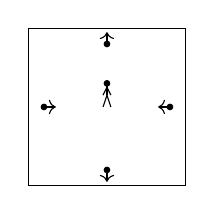
\begin{tikzpicture}
        \draw (-1,-1) -- (-1,1) -- (1,1) -- (1,-1) -- (-1,-1);
        \draw[fill=black] (0,0.3) circle (1pt);
        \draw (0,0.3) -- (0,0.15);
        \draw (0,0.15) -- (0.05,0);
        \draw (0,0.15) -- (-0.05,0);
        \draw (0,0.25) -- (0.05,0.15);
        \draw (0,0.25) -- (-0.05,0.15);
        \draw[fill=black] (-0.8,0) circle (1pt);
        \draw[fill=black] (0.8,0) circle (1pt);
        \draw[fill=black] (0,0.8) circle (1pt);
        \draw[fill=black] (0,-0.8) circle (1pt);
        \draw[->] (0,-0.8) -- (0,-0.95);
        \draw[->] (0,0.8) -- (0,0.95);
        \draw[->] (-0.8,0) -- (-0.65,0);
        \draw[->] (0.8,0) -- (0.65,0);
    \end{tikzpicture}
    \caption{Observer freely falling with particles experience tidal forces within the observers reference frame.}
\end{figure}
\begin{equation}
    \frac{d^2x^\mu}{d\tau^2} = 0
\end{equation} 
We can look at how this changes for the observer in a non-inertial frame.
\begin{equation}\label{eq:sr-curves}
    \frac{d^2x'^\lambda}{d\tau^2}+\underbrace{\frac{\partial x'^\lambda}{\partial x^\rho}\frac{\partial^2 x^\rho}{\partial x'^\mu \partial x'^\nu}}_{\equiv \Gamma_{\mu\nu}^\lambda} \frac{d x'^\mu}{d \tau} \frac{d x'^\nu}{d \tau} = 0
\end{equation}
Equation~\ref{eq:sr-curves} looks suspiciously like the geodesic equation from differential geometry. The exception is we have defined the `Chirstoffel symbol' here, which is not the most general form of the Christoffel symbols. This does give motivation for how to search for a compatible theory of gravity. However, this does provide a clear link between gravity and geometry. 
\section{Einstein's Field Equation}
Christoffel symbols take a very general form, where they signify the failure of partial derivatives to commute. This failure results from curvature of the space itself. As said in the previous section, special relativity promotes the classical $\mathbb{R}^3$ space to $\mathbb{M}^4$. However, we now need to allow curved space, not simply minkowski space. So lets take an arbitrary semi-Riemannian 4-manifold $M$. In very loose terms, a manifold is a locally euclidean space, which is a sufficient definition for this application.

Naturally, computing derivatives are difficult on curved surfaces. To start, derivatives give tangent vectors, thus taking the set of all possible tangent vectors of a curve at point $p\in M$ gives us the tangent space at $p$, denoted $T_pM$. The generalization of the derivative is called a \textit{connection}~\cite{baez_john_gauge_1994}, which tells one how to connect the tangent spaces at different points infinitessimally (figure~\ref{fig:parallel_transport}). Although beyond the scope of this thesis, it is worth noting that, due to the holonomy of curved surfaces, this will generally depend on the path taken.
\begin{figure}
    \centering
    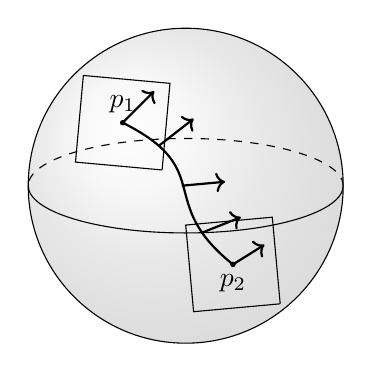
\begin{tikzpicture}
        \shade[ball color = gray!40, opacity = 0.2] (0,0) circle (2cm);
        \draw (0,0) circle (2cm);
        \draw (-2,0) arc (180:360:2 and 0.6);
        \draw[dashed] (2,0) arc (0:180:2 and 0.6);
        \fill[fill=black] (-0.8,0.8) circle (1pt);
        \draw (-0.8,0.8) node[anchor=south] {$p_1$};
        \fill[fill=black] (0.6,-1.0) circle (1pt);
        \draw (0.6,-1.0) node[anchor=north] {$p_2$};
        \draw (-0.8+0.5,0.8-0.6) -- (-0.8-0.6,0.8-0.5) -- (-0.8-0.5,0.8+0.6) -- (-0.8+0.6,0.8+0.5) -- (-0.8+0.5,0.8-0.6); %bottom right -- bottom left -- top left -- top right -- bottom right
        \draw (0.6+0.6,-1-0.5) -- (0.6-0.5,-1-0.6) -- (0.6-0.6,-1+0.5) -- (0.6+0.5,-1+0.6) -- (0.6+0.6,-1-0.5);
        \draw[thick] (-0.8,0.8) .. controls (0.4,0.2) and (-0.4,-0.2) .. (0.6,-1);
        \draw[->,thick] (-0.8,0.8) -- (-0.4,1.2);
        \draw[->,thick] (-0.35,0.5) -- (0.1,0.85);
        \draw[->,thick] (-0.05,0) -- (0.5,0.05);
        \draw[->,thick] (0.2,-0.6) -- (0.7,-0.4);
        \draw[->,thick] (0.6,-1) -- (1,-0.75);
    \end{tikzpicture}
    \caption{Example of parallel transport along a connection on a sphere. }
    \label{fig:parallel_transport}
\end{figure}
In general relativity, a very special connection is use called the \textit{Levi-Civita connection}, denoted $\nabla$, which is torsionless and metric preserving. More precisely, for all vector fields $u,v,w$ on $M$
\begin{equation}
    \begin{split}
        u g(v,w) =& g(\nabla_u v, w)+g(v,\nabla_uw) \,,\quad \text{(metric preserving)} \\
        [u,v] =& \nabla_u v - \nabla_v u \,,\quad \text{(torsion free)}
    \end{split}
\end{equation}

The only remaining geometric property for the Levi-Civita connection is curvature, which can be neatly described using the christoffel symbols defined by
\begin{equation}
    \nabla_\mu\partial_\nu = \Gamma^{\rho}_{\mu\nu}\partial_\rho\,.
\end{equation}
In this case, the partials here are refering to the basis of vector fields on $M$.Additionally this curvature has a special name as well, the \textit{Riemann curvature}, a type (3,1) tensor defined by
\begin{equation}
    R(u,v)w = (\nabla_u\nabla_v-\nabla_v\nabla_u - \nabla_{[u,v]})w
\end{equation}
or in coordinate form by
\begin{equation}
    R_{\mu\nu\rho}^\sigma  = \nabla_\mu \Gamma^\sigma_{\nu\rho} - \nabla_\nu\Gamma^{\sigma}_{\mu\rho}
\end{equation}
To emphasize the elegance of Einstein's equation, its convinient to note write the Riemann curvature as a matrix valued differential 2-form $\mathcal{R}$ and the christoffel symbols as a matrix valued differential 1-form $\mathcal{G}$ (differential forms are antisymmetric covariant tensors). With this notion, its easy to see the Bianchi identity for $\mathcal{R}$ with respect to the Levi-Civita connection is
\begin{equation}
    d_{\nabla}\mathcal{R} = \nabla_{[\tau}R^\sigma_{\mu\nu]\rho} = 0
\end{equation}
Where the brackets denote antisymmetric permutations of the indices. Working through the algebra gives
\begin{equation}
    \nabla^\mu G_{\mu\nu} = 0\quad G_{\mu\nu} = R_{\mu\nu}-\frac{1}{2}g_{\mu\nu}R
\end{equation}
Where $R$ and $R_\mu\nu$ are the Ricci scalar and Ricci tensor found by contracting indices in the Riemann tensor. This looks familiar to the conservation of energy equation
\begin{equation}
    \nabla^\mu T_{\mu\nu}=0
\end{equation}
Additionally, the metric itself is divergenceless. Putting these all together gives us Einstein's Field Equation
\begin{equation}
    G_{\mu\nu} + \Lambda g_{\mu\nu} = 8\pi\kappa T_{\mu\nu}
\end{equation}

\section{Cosmology}
We can see in Einstein's equation the constant $\Lambda$, called the cosmological constant. A great question in gravitational physics and cosmology is `what value does $\Lambda$ take, and what is its source'. The theory of $\Lambda$CDM, the standard model of cosmology, will be discussed, where dark matter is `cold' (so it clumps and forms halos) and dark energy acts as the cosmological constant ~\cite{scott_dodelson_modern_2021}.

When discussing $\Lambda$CDM (or cosmology in general), there are two main assumptions that are made on a global scale:
\begin{itemize}
    \item The universe is homogeneous. That is, there is no preferred location in the universe.
    \item The universe is isotropic. That is, there is no preferred direction of the universe.
\end{itemize}
Both of these assumptions should sound strange; Our universe is clearly does not follow these assumptions. If we look into the night sky, we can see regions of densly packed stars and galaxies and other regions with no stars or galaxies, violating the assumption of homogeneity (figure~\ref{fig:galaxy_map}). On the other hand, if one observes the temperature of the cosmic microwave background (CMB), one finds there is an angle dependence of the observed temperature (figure~\ref{fig:cmb_tt_map}), violating the assumption of isotropy. To reconsile this, the metric will be modified by perturbations. In this thesis, only scalar perturbations are considered.
\begin{figure}[ht]
    \centering
    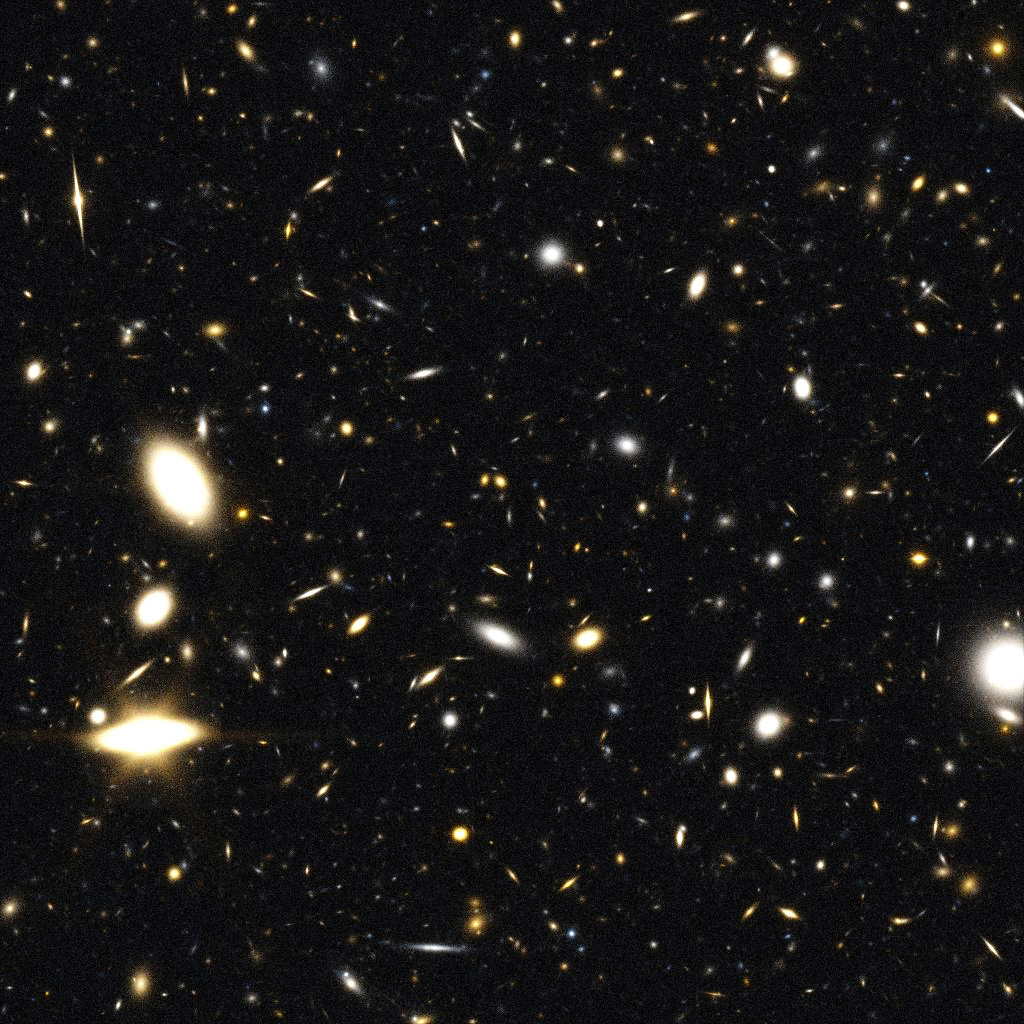
\includegraphics[width=0.75\textwidth]{plots/opo0220a.jpg}
    \caption{An image of galaxies from the James Webb Space Telescope, showing regions of high matter density and regions of low matter density.}
    \label{fig:galaxy_map}
\end{figure}
\begin{figure}[ht]
    \centering
    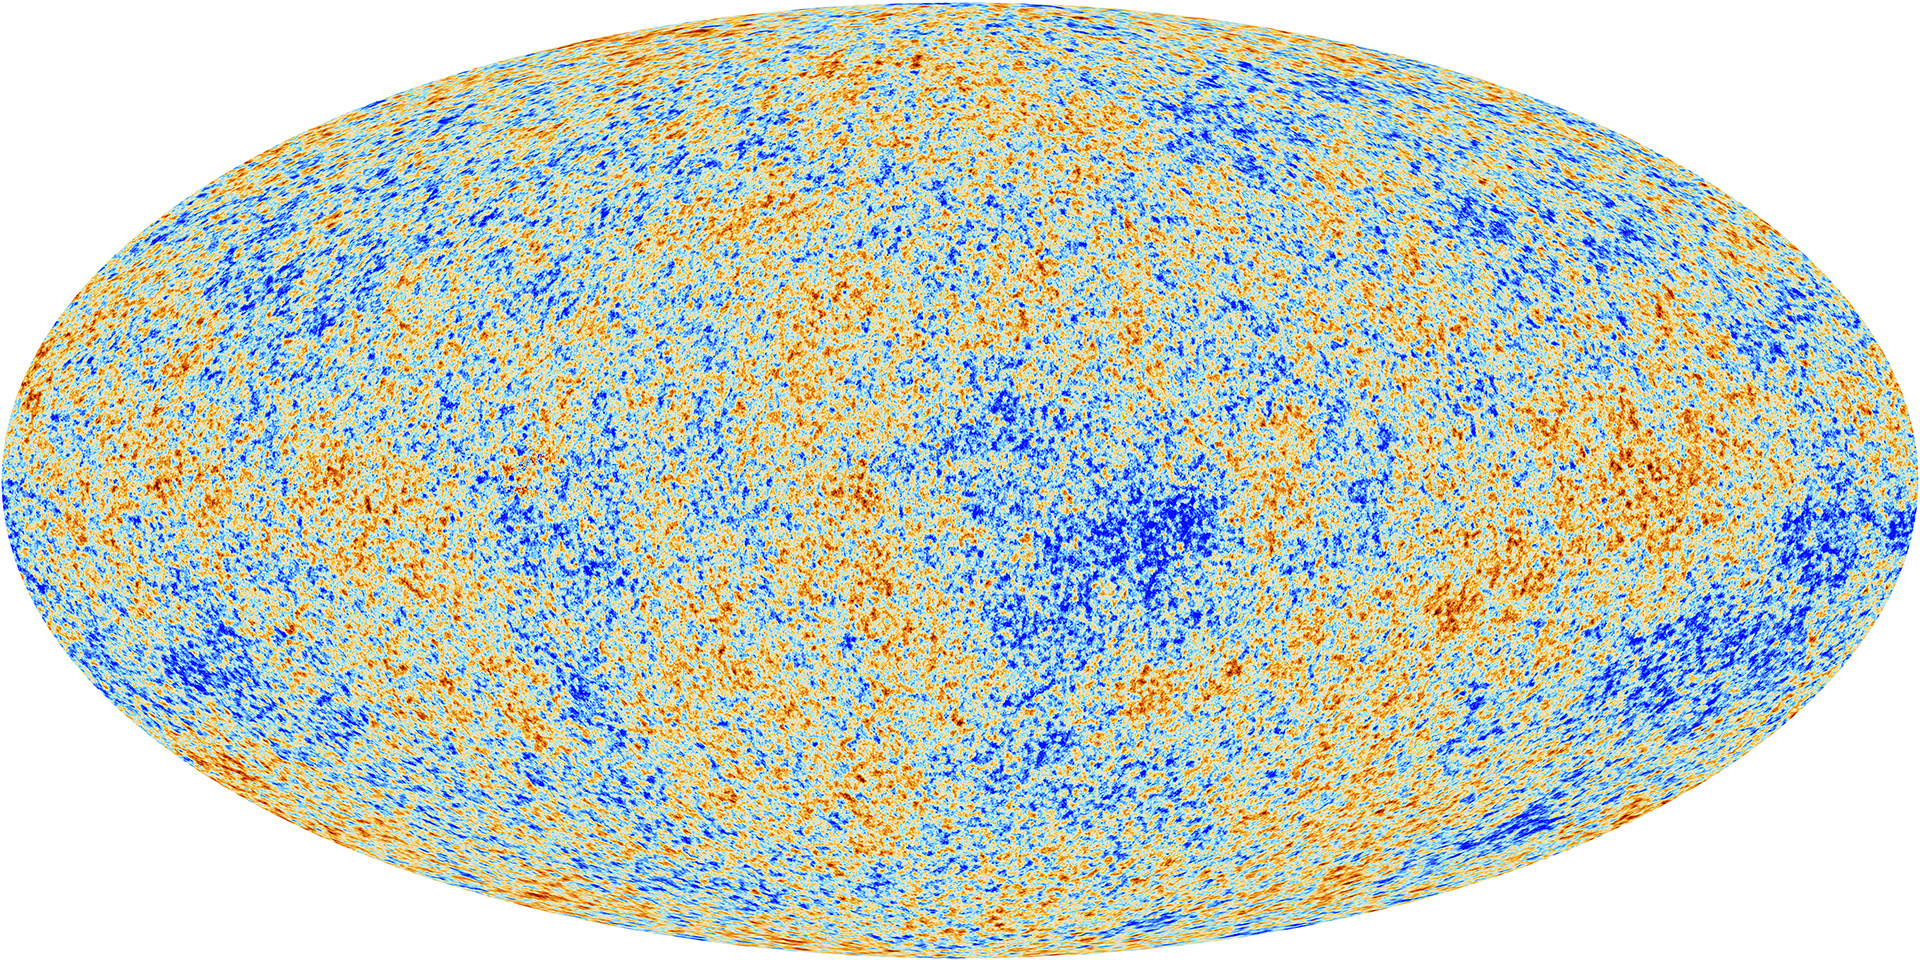
\includegraphics[width=0.75\textwidth]{plots/Planck_CMB.jpg}
    \caption{CMB TT power spectrum, emphasizing the scale of anisotropies.}
    \label{fig:cmb_tt_map}
\end{figure}

With Edwin Hubble's discovery of the expanding universe, any metric assigned to the universe must include homogeneous spatial expansion. Together with the above assumptions results in the FLRW metric.
\begin{equation}
    g = \text{diag}(-1,a^2,a^2,a^2)
\end{equation}
To perturb this metric around a homogenous universe, it requires two fields. The first, denoted $\Psi$, is the newtonian gravitational potential. Because newtonian gravity works in the non-relativistic limit, it enters the time component of the metric. The second field, denoted $\Phi$, represents spatial curvature perturbations. The perturbed metric is given by
\begin{equation}
    g = \text{diag}(-1-2\Psi,a^2(1-2\Phi),a^2(1-2\Phi),a^2(1-2\Phi))
\end{equation}
By computing the Christoffel symbols, one finds
\begin{equation}
    \begin{split}
        \Gamma^i_{00} = \frac{1}{a^2}\partial_i\Psi \\
        \Gamma^i_{0j} = \delta_{ij}(H+\dot\Phi) \\
        \Gamma^i_{jk} = (\delta_{ij} \partial_k + \delta_{ik}\partial_j - \delta_{jk}\partial_i)\Phi
    \end{split}
\end{equation}
Given Einstein's field equations and the perturbed FLRW metic, one can find the Friedman equations. The first comes from the 00 component of Einstein's field equations.
\begin{equation}
    H^2(t) = \frac{8\pi G}{3}\left(\rho + \frac{\Lambda}{8\pi G}\right) - \frac{k}{a^2}
\end{equation}
What can be done with this is to convert the curvature $k$ and the cosmological constant $\Lambda$ into densities as well, denoted $\rho_k$ and $\rho_\Lambda$ respectively. If those terms are absorbed into $\rho$, one finds
\begin{equation}
    H^2(t) = \frac{8\pi G}{3}\rho
\end{equation}
and the critical density is defined by the density associated with $H_0$,
\begin{equation}
    H_0^2 \equiv \frac{8\pi G}{3}\rho_{\text{crit}}
\end{equation}
Whats neat about this formulation with is that the value of the density today can tell us about the geometry of the universe. If $\rho>\rho_{\text{crit}}$ the curvature is positive (de Sitter geometry). If $\rho<\rho_{\text{crit}}$ the curvature is negative (anti-de Sitter geometry). If $\rho=\rho_{\text{crit}}$, the universe is flat. If we define the relative densities by
\begin{equation}
    \Omega_i = \frac{\rho_i}{\rho_\text{crit}}
\end{equation}
The relation becomes
\begin{equation}
    \Omega + \Omega_k = 1 
\end{equation}
Meaning if the non-curvature relative densities are less than 1, then the universe is curved with sign equal to the sign of $\Omega_k$.

The second Friedman equation comes from the trace of Einstein's equation.
\begin{equation}
    \frac{\ddot a}{a} = -\frac{4\pi G}{3}(\rho + 3P)
\end{equation}
In cosmology, there are other distances which can be more useful than the distance given by the FLRW metric. 
In the FLRW metric the distance between two points grows in time. 
We can avoid this by defining the \textit{comoving distance} in which distances remain fixed through time. 
If we look at a coordinate function $x^\mu$ at $t=t_0$, at a later time the coordinate function can be written as $x^\mu \rightarrow a(t) x^\mu$, thus by dividing by the scale factor $a(t)$ we can define the comoving coordinates as

\begin{equation}
    \chi = \int\limits^{t}_{t_0} \frac{1}{a(t')} dt'
\end{equation}

with the standard Minkowski metric. This can be taken a step further by determining how far light has travelled since $t=0$
\begin{equation}
    \eta = \int\limits^t_0 \frac{1}{a(t')}dt'
\end{equation}

Since we can't see anything beyond this distance, it is often called the \textit{comoving horizon}. 
There is one last useful distance to define, the \textit{angular distance} which is inferred by the angle subtended by two objects. 
This relates distances to the geometry discuss in the first section where the measured distance will be the radial distance $D$

\begin{equation}
    D_A = \left\{ \begin{array}{cc}
        R & K=0 \\
        R\sin(D/R) & K>0 \\
        R\sinh(D/R) & K<0
    \end{array}
    \right.
\end{equation}
\subsection{Cosmic Constituents of the Universe}
While we have made sense of the curvature density $\Omega_k$, there is still this mysterious $\Omega$ we see, which is a sum over other objects comprising the universe. Each of these objects are classified by their energy-momentum tensor and equation of state, defined by
\begin{equation}
    w_s = \frac{\mathcal{P}_s}{\rho_s}
\end{equation}
where $\mathcal{P}$ is the pressure and $\rho$ the density
\subsubsection{Radiation}
Radiation is defined to have 0 rest mass, and thus its energy-momentum is given by
\begin{equation}
    T = \text{diag}(\rho_\gamma, \rho_\gamma/3, \rho_\gamma/3, \rho_\gamma/3)
\end{equation}
(this can also be derived from Bose-Einstein statistics) Thus it has an equation of state $w_\gamma=1/3$. 

At one point, before recombination, radiation was the dominant component of the universe. As the universe cooled, the radiation was absorbed by the atoms forming until matter was the dominant. This formed the CMB which we measure today. Additionally, the CMB forms a nice black body, and thus the temperature can be found by measuring the emitted frequencies.
\subsubsection{Baryons}
Baryons are all non-relativistic particles which interact electromagnetically (so it excludes dark matter, but includes nuclei, electrons, etc.). Thus, its energy-momentum is given by
\begin{equation}
    T = \text{diag}(\rho_b,0,0,0)
\end{equation}
so its equation of state is given by $w=0$.
\subsubsection{Dark Matter}
Dark matter has the same energy-momentum as baryons, and thus the same equation of state. The main reason for the separation between Baryons and dark matter is that, experimentally, we can see baryons directly by imaging, but we cannot see dark matter. We can, however, see the gravitational effects of dark matter.
\subsubsection{Neutrinos}
Neutrinos are a special type of matter. They are relativistic $w=1/3$ but not radiation. Their energy-momentum can be computed the same way as for photons, but using Fermi-Dirac statistics. The density is thus
\begin{equation}
    \rho_\nu = \frac{21}{8}\left(\frac{T_\nu}{T}\right)^4\rho_\gamma
\end{equation}
\subsubsection{Dark Energy}
Dark energy is a special component of the universe. It is like a cosmological constant, and thus the energy momentum tensor is
\begin{equation}
    T = \text{diag}(\rho_\Lambda,-\rho_\Lambda,-\rho_\Lambda,-\rho_\Lambda)
\end{equation}
as such, its equation of state is $w=-1$

\chapter{Measurement of Weak Lensing and the Cosmic Microwave Background}
\section{Weak Lensing}
In general, contemporary weak lensing surveys measure the light emitted from galaxies in two components: galaxy position and galaxy shear. In the following sections, the theoretical base for cosmological weak lensing surveys are described. However, before discussing the two relevant observables, one needs to formalize the concept of weak lensing.
\begin{figure}[ht]
	\centering
	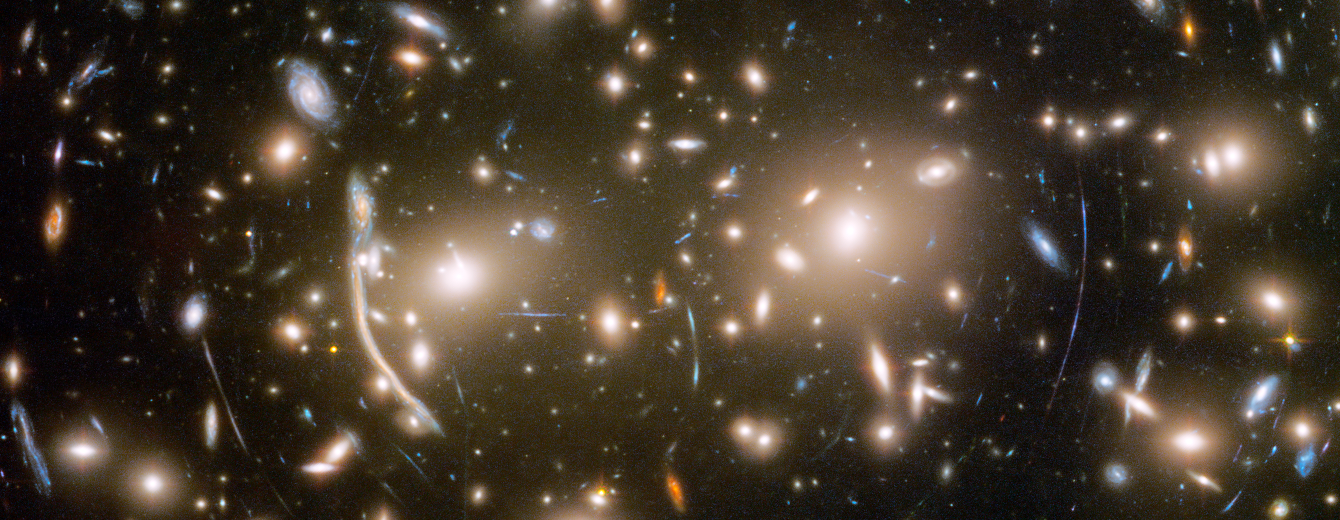
\includegraphics[width=\textwidth]{plots/hubble_weak_lensing.png}
	\caption{Image of weak lensing taken by the Hubble Space Telescope~\cite{hubble_lensing}.}
	\label{fig:weak_lensing}
\end{figure}
\subsection{The Linear Matter Power Spectrum}
As we have seen before, we consider deviations from the FLRW metric using the scalar fields $\Phi$ and $\Psi$. In the absence of anisotropic stress, $\Phi=-\Psi$, which we will assume here for demonstration (one can use codes such as CAMB or CLASS to do computations including anisotropy if desired). 

Throughout time in the universe, we consider there to be three distinct epochs or regions~\cite{scott_dodelson_modern_2021}:
\begin{itemize}
	\item The super-horizon region, or the region before inflation where radiation dominates
	\item The horizon-crossing region, or the region during inflation where the universe transfers from radiation to matter domination
	\item The sub-horizon region, or the region of after rapid inflation where matter dominates
\end{itemize}
Additionally, the formation of matter inhomogeneity comes from gravitational instability, the idea that primordial curvature perturbations in the super-horizon grew to form small matter density contrasts which grew after crossing the horizon. After the rate of inflation slowed, gravitational forces caused clusters of matter to become the galaxies and clusters we see today.

This gives us a blueprint for writing the matter power spectrum. We have the primordial curvature perturbation $\mathcal{R}$ which source the initial matter inhomogeneity that formed late-time large scale structure. Thus, we can write it as
\begin{equation}
	\mathcal{R} = \frac{5}{3}\Phi_{\text{large-scale}}(k,a_{\text{late}})\,.
\end{equation} 
Additionally, we have a transfer function which describes the transition from radiation to matter domination, defined as
\begin{equation}
	T(k) = \frac{\Phi(k,a_{\text{late}})}{\Phi_{\text{large-scale}(k,a_{\text{late}})}}\,.
\end{equation}
And we have a growth factor, defined as the linear growth of matter density contrast during matter domination, defined as
\begin{equation}
	D_+(a) = a \frac{\Phi(k,a)}{\Phi(k,a_{\text{late}})}\,.
\end{equation}
Thus we can write the gravitational potential at all times as
\begin{equation}
	\Phi(k,a) = \frac{3}{5a}\mathcal{R}(k)T(k,a)D_+(a)\,.
\end{equation}
This together with the Poisson equation for the matter density contrast field gives the equation
\begin{equation}
	\delta_m(k) = \frac{2k^2a}{3\Omega_mH_0^2}\Phi(k,a)\,,
\end{equation}
\begin{equation}
	\delta_m(k) = \frac{2}{5}\frac{k^2}{\Omega_mH_0^2}\mathcal{R}(k)T(k,a)D_+(a)\,,
\end{equation}
The power spectrum of an observable is defined as the two-point correlation function of the observable in Fourier space.
\begin{equation}
	P_\mathcal{O}(k) = \langle \mathcal{O}(k)\mathcal{O}(k) \rangle\,.
\end{equation}
Thus, the linear matter power spectrum (because we restricted the matter density contrast field to linear order terms in the perturbation) is given by
\begin{equation}
	\begin{split}
		P_m^{L}(k,a) = \frac{8\pi^2}{25 \Omega_m^2 H_0^4} A_s D_+^2(a)T^2(k)\frac{k^{n_s}}{k_p^{(n_s-1)}}\,.
	\end{split}
\end{equation}

\subsection{Galaxy Density}
In practice, we cannot measure the matter power spectrum; Dark matter prohibits direct measurement. Instead, one must determine observables which trace the matter distribution in the universe. The most natural option is to observe the galaxy distribution. However, large scale structures and galaxies provide many sources for non-linearities in the power spectrum and result in a non-trivial relation between the two. By taking certain data selection criteria, one can cut out the non-linear contributions. The relation between the galaxy and matter power spectra are then related by the linear bias factor.
\begin{equation}
	\begin{split}
		\delta_g(k) &= b_1 \delta_m(k) \\
		P_g(k,a) &= (b_1)^2P_m^L(k,a)\,.
	\end{split}
\end{equation}
Realistically, in galaxy surveys, we do not have access to exact redshifts for each observed galaxy. Rather, an image is taken of the sky in multiple color bands, from which the redshift is determined. This procedure is called photometric redshift. To account for this, one can attempt to redefine the galaxy power spectrum. First, we define the distribution of distances, as
\begin{equation}
	W(\chi) = \frac{1}{N_g}\frac{dN_g}{d\chi}\,.
\end{equation}
The procedure for determining this distribution will be discussed in sections~\ref{sec:dz} and~\ref{sec:IA}. This allows us to simply write the projected density contrast as
\begin{equation}
	\Delta_g = \int\limits_0^\infty W(\chi)\delta_g(x,\tau)d\chi\,.
\end{equation}
To complete this discussion, we will make some approximations. The first is that we will only consider small scales for which $\sin(\theta)\sim \theta \sim 1/l$ where $l$ is the Fourier conjugate of $\theta$. The second is the limber approximation, which states that, as long as the galaxy power spectrum $P_g$ slowly varies over the region $\Delta k \sim 1/l\chi$, we approximate is as a constant. These approximations greatly simplify the integrals required when computing the power spectrum of the Fourier transformed $\Delta_g$. This power spectrum is called the angular power spectrum. Considering the approximations above and computing the Fourier transform, one finds an angular power spectrum of
\begin{equation}
 	C_g(l) =\int \frac{1}{\chi^2}W^2(\chi)P_g(k=(l+1/2)/\chi,\eta) d\chi\,.
\end{equation} 
\subsection{Galaxy Shear}
Photons move on null geodesics, thus $d\chi = -d\eta$, where $\eta$ is the conformal time and $\chi$ is the conformal distance. This tells us that, through some changes of variables, $dx^i/d\chi = -\hat{p}^i$ (for photons and other massless particles). Thus, under lensing, the difference between the observed and true positions within the source plane is given by
\begin{equation}
	\chi\mathbf{\theta}^i = x_\perp^i = -\int\limits_0^\chi \hat{p}^i_\perp(\chi'') d\chi''\,.
\end{equation}
The goal is to write this as a function of the potential only. Thus, we look to compute $d\hat{p}^i/dt$.
\begin{equation}\label{eq:dp-hat-dt}
	\begin{split}
		\frac{d\hat{p}^i}{dt} %=& \frac{d}{dt}\frac{1}{p}p^i \\
		=& \frac{1}{p^2}(\dot{p}^i p - \dot{p}p^i)\,.
	\end{split}
\end{equation}
By computing $\dot p^i$, one can find $\dot p$ as well:
\begin{equation}
	\begin{split}
		\frac{dp^i}{d\lambda} %=& \frac{d}{d\lambda}\left(aP^i(1+\Phi)\right) \\
		=& P^i\frac{d}{d\lambda}(a(1+\Phi)+(1+\Phi)a\frac{d}{d\lambda}P^i\,.
	\end{split}
\end{equation}
Also, $d/d\lambda = P^\mu \partial_\mu$, so the first term becomes
\begin{equation}
	\begin{split}
		P^i\frac{d}{d\lambda}(a(1+\Phi)) %&= P^iP^\mu \partial_\mu(a(1+\Phi)) \\
		%&= P^iP^0(\dot a + a\dot\Phi + \dot a \Phi) + a P^iP^j \partial_j\Phi \\
		&= a P^i (P^0(H+\dot\Phi +H\Phi) + P^j\partial_j\Phi)\,. \\
	\end{split}
\end{equation}
The second term is evaluated by using the geodesic equation up to first order in the perturbations $\Phi$ and $\Psi$.
\begin{equation}
	\begin{split}
		\frac{d}{d\lambda}P^i &= -\Gamma^i_{\mu\nu}P^\mu P^\nu \\
		%&= -(P^0)^2\frac{1}{a^2}\partial^i\Psi - 2\delta^{i}_{j}(H+\dot\Phi)P^0P^j + 2P^iP^j\partial_j\Phi - P^jP_j\partial^i\Phi \\
		%&= -E(1-\Psi)\left( \frac{E}{a^2} \partial^i\Psi + \frac{1}{a}2p^i(1-\Phi)(H+\dot\Phi) - \frac{2}{a^2E}p^ip^j\partial_j\Phi + \frac{p^2}{a^2E} \partial^i\Phi \right) \\
		&= -E\left( \frac{E}{a^2} \partial^i\Psi + \frac{1}{a}2p^i(1-\Phi-\Psi)(H+\dot\Phi) - \frac{2}{a^2E}p^ip^j\partial_j\Phi + \frac{p^2}{a^2E} \partial^i\Phi \right)\,.
	\end{split}
\end{equation}
Plugging everything back in, and only keeping terms to linear order, one gets
\begin{equation}
	\begin{split}
		%=& aP^i(H+\dot\Phi+H\Phi) + aP^iP^j\partial_j\Phi \\
		%& - \frac{E}{a}\partial^i\Psi - 2p^i(H+\dot\Phi) + \frac{2}{aE}p^ip^j \partial_j\Phi - \frac{p^2}{aE}\partial^i\Phi \\
		\frac{dp^i}{dt} %=& p^i(1-\Phi)(H+\dot\Phi+H\Phi) + (1-\Phi)^2p^ip^j\partial_j\Phi \\
		%& - \frac{E}{a^2}\partial^i\Psi -\frac{2p^i}{a}(H+\dot\Phi) + \frac{2}{a^2E}p^ip^j \partial_j\Phi - \frac{p^2}{a^2E}\partial^i\Phi \\
		%=& p^i(H+\dot\Phi) + \frac{p^ip^j}{aE}\partial_j\Phi \\
		%& - \frac{E}{a}\partial^i\Psi -2p^i(H+\dot\Phi) + \frac{2}{aE}p^ip^j \partial_j\Phi - \frac{p^2}{aE}\partial^i\Phi \\
		=& -p^i(H+\dot\Phi)- \frac{1}{aE}\left(p^ip^j\partial_j\Phi - p^2\partial^i\Phi\right) -\frac{E}{a}\partial^i\Psi\,.
	\end{split}
\end{equation}
The time derivative of the modulus of the momentum, $p$, is then given by
\begin{equation}
	\begin{split}
		\frac{dp}{dt} =& \frac{d}{dt}\sqrt{\delta_{ij}p^ip^j} = \frac{1}{p}\delta_{ij}\dot p^i p^j \\
		%=& -p(H+\dot\Phi) - \frac{p}{aE}(p^i\partial_i\Phi - pp^i\partial^i\Phi) - p^i\frac{E}{ap}\partial^i\Psi \\
		=& -p(H+\dot\Phi) - \hat{p}_i\frac{E}{a}\partial^i\Psi\,.
	\end{split}
\end{equation}
Now, putting everything together, plugging these results into eq~\ref{eq:dp-hat-dt} gives
\begin{equation}
	\begin{split}
		\frac{d\hat{p}^i}{dt} %=& -\hat{p}^i(H+\dot\Phi)- \frac{1}{aEp}\left(p^ip^j\partial_j\Phi - p\partial^i\Phi\right) -\frac{E}{ap}\partial^i\Psi + \hat{p}^i\left( (H+\dot\Phi) + \hat{p}_i\frac{E}{ap^2}\partial^i\Psi \right) \\
		=&  \frac{E}{ap}\left( \frac{p^2}{E^2}\partial_j\Phi - \partial_j\Psi \right)(\delta^{ij}-\hat{p}^i\hat{p}^j)\,.
	\end{split}
\end{equation} 
Going back to the photon scenario, where $E=p$, this simplifies to
\begin{equation}
	\frac{d\hat{p}^i}{dt} = \frac{1}{a}\left( \partial_j\Phi - \partial_j\Psi \right)(\delta^{ij}-\hat{p}^i\hat{p}^j)\,.
\end{equation}
Interestingly, $\delta^{ij}-\hat p^i \hat p^j$, is the projection operator of the $j$-th direction onto the $i$-th. So, if we orient our axes so that the photon approximately travels along the $j$-th direction, we can sum of $i$ and $k$ so that the orthogonal components of the momentum are evaluated by
\begin{equation}
	\frac{d\hat{p}^i_\perp}{d\chi} = - a \frac{d\hat{p}^i_\perp}{dt} = -\partial_i(\Phi-\Psi)
\end{equation}
In the absence of anisotropic stress (like in the late universe where weak lensing is measured), $\Phi=-\Psi$ and 
\begin{equation}
	\frac{d\hat{p}^i_\perp}{d\chi} -2\partial_i\Phi\,.
\end{equation}
Integrating this equation gives
\begin{equation}
	\hat p_\perp (\chi'') = -2\int\limits_0^{\chi''}\partial_i\Phi(\chi') d\chi' + C_i\,,
\end{equation}
where the constant $C_i$ comes from integrating a derivative, where it is only defined up to a constant. Now, plugging this back in one finds
\begin{equation}
	\mathbf{\theta}^i = \frac{2}{\chi}\int\limits_0^\chi \int\limits_0^{\chi''}\partial_i\Phi(\chi') d\chi' d\chi'' - C_i\,.
\end{equation}
In the absence of lensing, this should reduce to $\mathbf{\theta}^i = \theta_0$, the true source position. Hence $C^i=\theta^i_0$ and the total deflection angle is given by
\begin{equation}
	\begin{split}
		\Delta\theta^i =& \frac{2}{\chi}\int\limits_0^\chi \int\limits_0^{\chi''}\partial_i\Phi(\chi') d\chi' d\chi''\\
		=& \frac{2}{\chi}\int\limits_0^\chi \partial_i\Phi(\chi') (\chi-\chi') d\chi'\,.
	\end{split}
\end{equation}
Finally, since $x^i=\chi\theta^i$, $\partial_i = \partial_{\theta^i}/\chi$. Introduce the \textit{lensing potential} defined by
\begin{equation}
	\begin{split}
		\Delta\theta^i =& \frac{\partial}{\partial \theta^i}\psi_L(\theta) \\
		\psi_L(\theta) =& 2\int\limits_0^\chi \frac{1}{\chi'}\Phi(\chi') \left(1-\frac{\chi'}{\chi}\right) d\chi'\,.
	\end{split}
\end{equation}
This result is great, but it's not very experimentally illuminating. Similar to the galaxy versus matter power spectrum, the absence of the observation of dark matter means we cannot reliably determine the potential $\Phi$. Again, an attempt to relate the lensing potential to some property of galaxies can give us a measurable quantity. Lensing distorts the shape of the galaxies (see figure~\ref{fig:weak_lensing}), where we assume all galaxies are elliptical. Define the galaxy shape tensor by
\begin{equation}
	q_{ij} \equiv \frac{1}{F}\int I\theta^i\theta^j d\theta^i d\theta^j\,.
\end{equation}
This integral is symmetric under $i \leftrightarrow j$. Writing this as a matrix gives
\begin{equation}
	q_{ij} = \frac{1}{2} \text{tr}(q) \left( 
	\begin{array}{cc}
	1+\epsilon_1 & \epsilon_2 \\
	\epsilon_2 & 1-\epsilon_1
	\end{array}
	\right)\,.
\end{equation}
Shape distortion occurs when the deflection angle is not constant across a galaxy. We can look at the transformation tensor as
\begin{equation}
	A_{ij} \equiv \frac{\partial \theta^i_S}{\partial\theta^j} = \left( 
	\begin{array}{cc}
	1+\kappa - \gamma_+ & -\gamma_\times \\
	-\gamma_\times & 1+\kappa+\gamma_+
	\end{array}
	\right) = \delta_{ij}+\psi_{ij}\,.
\end{equation}
Within this tensor, the $\gamma_+$ and $\gamma_-$ terms represent shear and $\kappa$ represents magnification and changes in galaxy light flux ($F$). The $E$-mode is given by
\begin{equation}
	E(l) = \left( \frac{l^il^j}{l^2} - \frac{1}{2}\delta^{ij} \right)(-\psi^{ij}(l))\,.
\end{equation}
Which relates to the shear components by
\begin{equation}
	\left(
	\begin{array}{c}
	\gamma_+ \\
	\gamma_\times
	\end{array}
	\right)
	=
	\left(
	\begin{array}{c}
	\cos(2\alpha_l) \\
	\sin(2\alpha_l)
	\end{array}
	\right)
	E(l)\,.
\end{equation}
This connects the observable shear to the theoretical lensing potential.
\subsection{Weak Lensing Correlation Functions}
In the previous two sections, we have derived two observables directly connected to cosmological theories. By observing the galaxies we can determine $\Omega_b$, $A_s$, $n_s$ and $H_0$. By observing shear, we can determine $\Omega_m$. The details of how to determine these parameters will be discussed in chapter 3. Together, these two can fully determine the values of the 5 $\Lambda$CDM parameters. These two quantities themselves are not observables. Using these two quantities, however, one can construct three different two-point correlation functions which are observable.

The first correlation function is the autocorrelation of galaxy density, called galaxy clustering. Given a density in a particular angular position, the correlation function can be interpreted as the likelihood of observing a similar density at another close position. The galaxy clustering correlation function is given by
\begin{equation}
	w_g(\theta) = \mathcal{F}(C_g(l)) = \frac{1}{2\pi}\int\limits_0^\infty l C_g(l) J_0(l\theta)dl\,,
\end{equation}
where $J_0$ is the 0-th Bessel function and $\mathcal{F}$ denotes the Fourier transform.

Next is the shear autocorrelation. In this case, there are two components of shear: the tangential shear $\gamma_+$ and the cross shear $\gamma_\times$. The cross correlation $\langle \gamma_+ \gamma_\times \rangle$ vanishes, and the remaining combinations are
\begin{equation}
	\begin{split}
		\langle \gamma_+\gamma_+ \rangle \pm \langle \gamma_\times \gamma_\times \rangle = \xi_\pm
	\end{split}
\end{equation}
\begin{equation}
	\xi_{+,-} = \frac{1}{2\pi}\int\limits_0^\infty l C_{EE}(l) J_{0,4}(l\theta)C_{EE}(l)dl\,.
\end{equation}

The final observable is the cross correlation between galaxy density and tangential shear. First, the angular power spectrum $C_{gE}(l)$ is given by
\begin{equation}
	C_{gE}(l) = \frac{3}{2}\Omega_mH_0^2 \int\limits_0^\infty \frac{1}{\chi a(\chi)}W_g(\chi)P_g(k,\eta) d\chi\,.
\end{equation}
\begin{equation}
	\gamma = \langle \Delta_g\gamma_+\rangle = -\frac{1}{2\pi}\int\limits_0^\infty l J_2(l\theta)C_{gE}(l)dl\,.
\end{equation}
The correlation function $\langle \Delta_g\gamma_\times\rangle$ vanishes in an isotropic universe.

\subsection{Systematics}
Up to now, we have neglected any systematics of the weak lensing observables. There are two distinct types of systematics that will be discussed in this section: The ones which affect the calculation of the correlation functions, and the ones which affect the correlation functions after they have been computed. The latter type of parameters are usually referred to as `fast' parameters, and it will become clear why that is in the next chapter. In the meantime, here is an explanation of the relevant systematics.
\subsubsection{Photometric Redshift Uncertainty}\label{sec:dz}
To compute the two-point correlation functions, one must determine the redshift distribution $W(\chi)$. This is a highly non-trivial task. To model the uncertainty in this distribution, one applies a constant shift to the redshift of observed galaxies.
\begin{equation}
	n_g(z) \mapsto n_g(z+\Delta z)
\end{equation}
The shift $\Delta z$ must be determined before one can compute the galaxy clustering and galaxy lensing correlation functions.
\subsubsection{Intrinsic Alignment of Galaxies}\label{sec:IA}
As can be seen in figure (fig), galaxy shapes are not completely random. In the absence of lensing, there is still some non-zero correlation between the shapes. This is referred to as Intrinsic Alignment~\cite{troxel_intrinsic_2015,scott_dodelson_modern_2021}. There are two models of intrinsic alignment that will be considered in this thesis: the Tidal Alignment Tidal Torquing (TATT) model~\cite{krause_dark_2021,blazek_beyond_2019} and the Non-linear Alignment (NLA) model. The TATT depends on the tidal tensor $s_{ij}$, which contains the information about tidal forces due to non-uniform gravitational fields. Tidal forces are a source of intrinsic alignment and shear (figure). The model is given by
\begin{equation}
	\gamma_{ij}^I = \underbrace{C_1s_{ij}}_{\text{tidal alignment}}+
	\underbrace{b_{TA}C_1(\delta_m\times s_{ij})}_{\text{density weighting}}+
	\underbrace{C_2\left( s_i^ks_{kj}-\frac{1}{3}\delta_{ij}s^2 \right)}_{\text{tidal torquing}}\,,
\end{equation}
where the coefficients $C_a$ are given by
\begin{equation}
	\begin{split}
		C_1 =& -\frac{A_1\bar{C}\Omega_m}{aG(z)}\left(\frac{1+z}{1+z_0}\right)^{\eta_1} \\
		C_2 =& 5\frac{A_2\bar{C}\Omega_m}{(aG(z))^2}\left(\frac{1+z}{1+z_0}\right)^{\eta_2}\,.
	\end{split}
\end{equation}
The TATT model reduces to the NLA model when $A_2=0=b_{TA}$.
\subsubsection{Galaxy Bias}
As discussed in the galaxy clustering section, we relate the galaxy and matter density by a bias parameter $b$. However, we can pick a fiducial value to relate the two
\begin{equation}
	\delta_{g,\text{fid}} = b_{\text{fid}}\delta_m
\end{equation}
then consider a multiplicative deviation:
\begin{equation}
	\delta_g = (b\cdot b_{\text{fid}})\delta_m = b\delta_{g,\text{fid}}\,.
\end{equation}
Thus, the parameter $b$ can be found to account for different galaxy biases. 

Galaxy bias is the first of many `fast' parameters. Since the bias is constant, it can be pulled out of the integral for the correlation functions, meaning it can be applied after the correlation function has been computed. The affected correlation functions are the galaxy clustering and galaxy-galaxy lensing.
\begin{equation}
	\begin{split}
		w^i(\theta) =& b_{(i)}^2w^i(\theta) \\
		\gamma^i_t(\theta) =& b_{(i)}\gamma_t^i(\theta)\,.
	\end{split}
\end{equation}
where $i$ denotes the redshift bin.
\subsubsection{Shear Calibration}
Observed shear is not a completely astrophysical phenomenon. For example, a major source of additional shear comes from the observation lens itself, where the observed galaxy shape is given by the true galaxy shape convolved with the point spread function of the lens~\cite{hirata_shear_2003,gillis_effects_2019}. This is usually modelled as a multiplicative correction to the shear components.
\begin{equation}
	\begin{split}
		\xi^{ij}_{\pm} =& (1+m^i)(1+m^j) \xi^{ij}_{\pm} \\
		\gamma^{ij}_t =& (1+m^j) \gamma_t^{ij}\,,
	\end{split}
\end{equation}
where $i$ and $j$ denote the source and lens bin respectively. The multiplicative shear calibration is also a fast parameter.
\subsubsection{Point Mass}
Currently, we are unable to model the contribution of small scales to the tangential shear~\cite{maccrann_controlling_2020}. The tangential shear can be written in terms of the surface mass density $\Sigma$ in the tangential direction:
\begin{equation}
	\gamma_t(R/D_A) = \frac{\bar\Sigma(0,R) - \Sigma(R)}{\Sigma_\mathrm{crit}} = \frac{\Delta\Sigma(R)}{\Sigma_\mathrm{crit}}\,.
\end{equation}
We can only model the tangential shear to $r_\mathrm{min}$, which allows us to write the point mass contribution (named for the $R^{-2}$ dependence) as
\begin{equation}
	\Delta\Sigma(R) = \Delta\Sigma^{\mathrm{model}}(R) + \frac{B}{R^2}\,.
\end{equation}
\subsubsection{Lensing Magnification}
In weak lensing, the intrinsic shape of galaxies also gets magnified. This effect is introduced as a parameter $C_l^i$ and is fixed experimentally.

%Additionally, DES added a non-physical parameter called $X_{\text{lens}}$ to resolve an inconsistency between two lensing samples, RedMaGiC and MagLim. In this thesis, we only consider $X_{\text{\lens}}=1$

\section{CMB}
Although CMB data is not used very much in this thesis, it is worth discussing the measurements qualitatively. The consensus among physicists and astronomers that the universe beyond the horizon was a hot, dense plasma. As such, the mean free path of photons was much shorter than it is today, and thus Compton scattering dominated photon dynamics in the early universe. As the universe cooled, atoms began to form in a process called recombination~\cite{scott_dodelson_modern_2021,hu_animations_nodate}. During this time, the universe was still opaque as photons scattered on the newly formed atoms. As the universe began to expand, the mean free path of photons increased and inter-atomic interactions decreased, meaning the atoms could be ionized by absorbing free photons in a process called reionization. The absorption of the photons caused the universe to become transparent. One can compute the optical depth of this transition from opaque to transparent as
\begin{equation}
	T = T_0(1-e^{-\tau_{\mathrm{rei}}})\,.
\end{equation}
$\tau_{\mathrm{rei}}$ concludes the introduction of cosmological parameters. $\tau_{\mathrm{rei}}$ can only be determined from CMB and is usually fixed in weak lensing analysis.

The CMB is a black body, meaning the intensity of the light can be used to determine the temperature according to the black body equation where $I \propto T^4$. The temperature, along with the $E$-mode polarization, gives three possible two point correlation functions: $TT$, $TE$, and $EE$.
\subsection{TT Power Spectrum}
\begin{figure}
    \centering
    \includegraphics[width=12cm]{plots/Planck_TT.png}
    \caption{Planck TT power spectrum}
    \label{fig:planck_tt}
\end{figure}
The TT power spectrum measures the anisotropies of the temperature field. Thus, it is better to consider it as the deviation from the mean temperature. There are some prominent features of this spectrum worth discussing. The first is the oscillations, known as baryon acoustic oscillations. The second is the overall downward trend from large to small scales. This is generally due to diffusion of light through the early universe, and is given the name diffusion damping.

Now one can observe qualitatively how the cosmological parameters will affect the TT power spectrum. First, consider $\Omega_b$, the baryon density. If the density is increased, there should be an increase in Compton scattering and decrease in the mean free path of photons, meaning the large scale anisotropy will be larger. Inversely, a reduction in the baryon density would decrease the large scale anisotropy. This is typically observed as the height of the first peak in the TT power spectrum. There will also be a small change in the peak position due to the change in the sound horizon. The height of the second peak, however, decreases. This is due to the increased pressure, which drives down the overall temperature fluctuations, resulting in every other peak changing in opposite directions.

Next is to consider a change is $\Omega_c$. The dominant effect from changing $\Omega_c$ comes from the integrated Sachs-Wolfe (ISW) effect, which is an additional gravitational redshift that occurs between the time of reionization and now. Since the evolution of dark matter structure is slow, increasing $\Omega_c$ reduces the ISW effect, thus reducing the anisotropy and causing an overall downward shift in the TT power spectrum.

The remaining parameters are considered in unison: $\mathcal{A}_s$, $n_s$, and $\tau_{\mathrm{rei}}$. Naturally, $\tau_{\mathrm{rei}}$ will have an overall suppression effect, The higher the anisotropy, the higher the suppression, thus resulting in strong suppression at large scales and weak suppression at small scales. The amplitude and spectral index enter the power spectrum similarly to how they did for weak lensing. Thus, the effect of $\mathcal{A}_s$ and $n_s$ can look identical to changes in $\tau_\mathrm{rei}$.

Finally, is a consideration of $H_0$, the most simple case. $H_0$ affects the expansion rate of the universe, thus a changing the value of $H_0$ will shift the position of the peaks in the power spectrum. Increases in $H_0$ will shift the peaks to smaller scales (found by propagating $H_0$ backward through time), and inversely, lowering $H_0$ will shift the peaks to larger scales. Additionally, the peaks at small scales will have a lower shift than the peaks at large scales. Hence, $H_0$ can also be determined by the distance between the peaks.
\subsection{TE and EE Power Spectra}
\begin{figure}
    \centering
    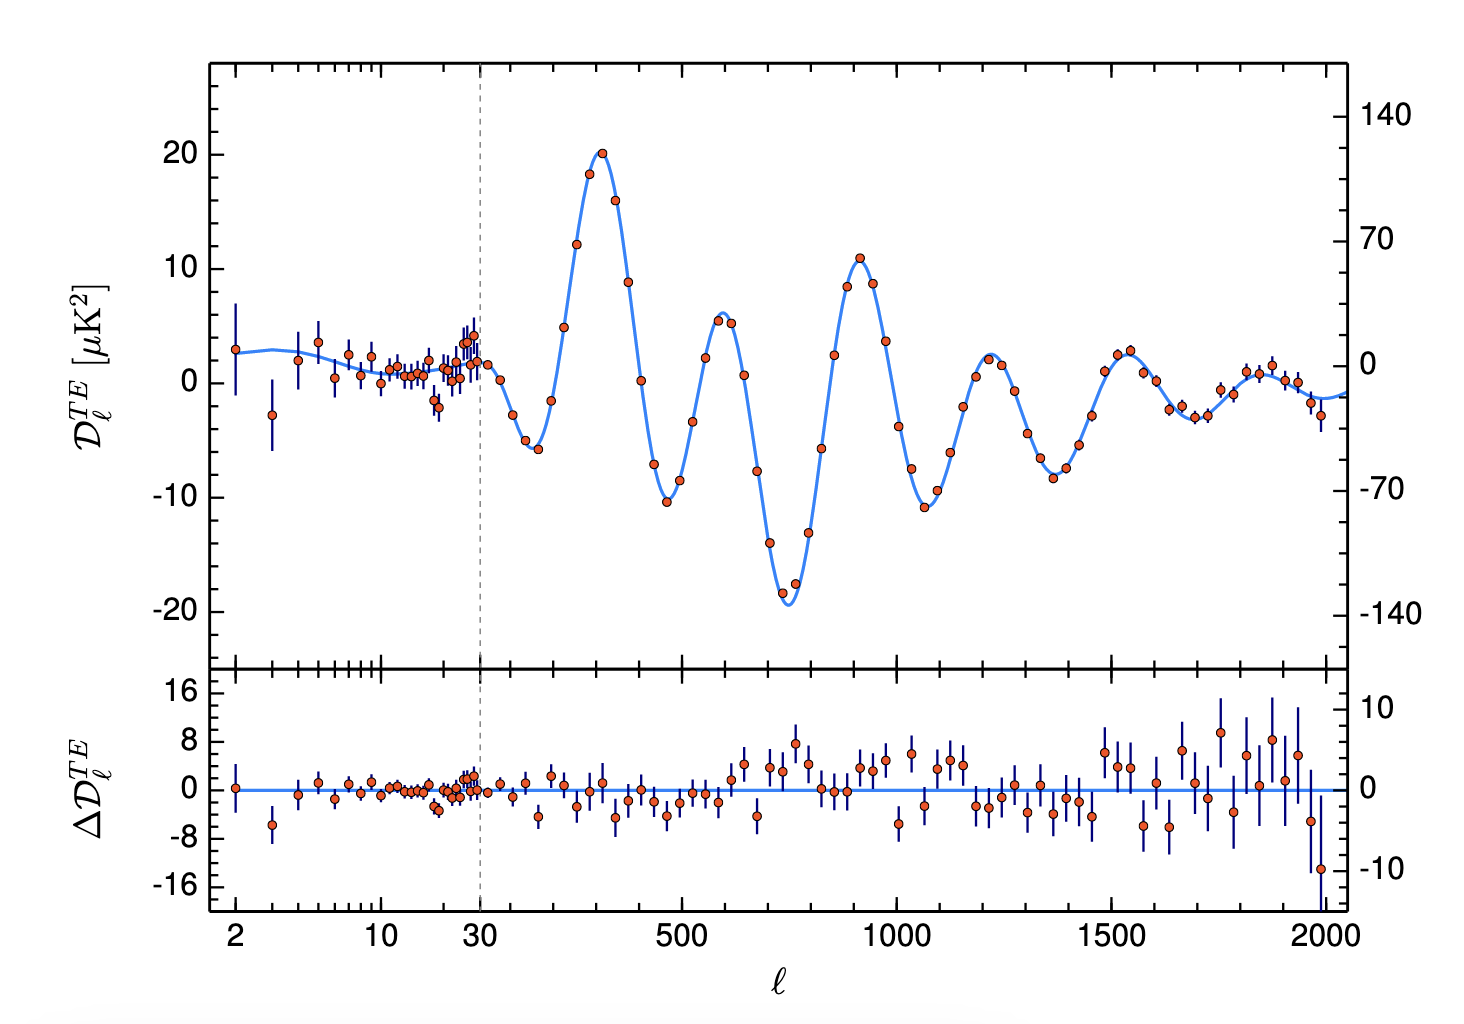
\includegraphics[width=12cm]{plots/planck_TE.png}
    \caption{Planck TE power spectrum}
    \label{fig:planck_te}
\end{figure}
\begin{figure}
    \centering
    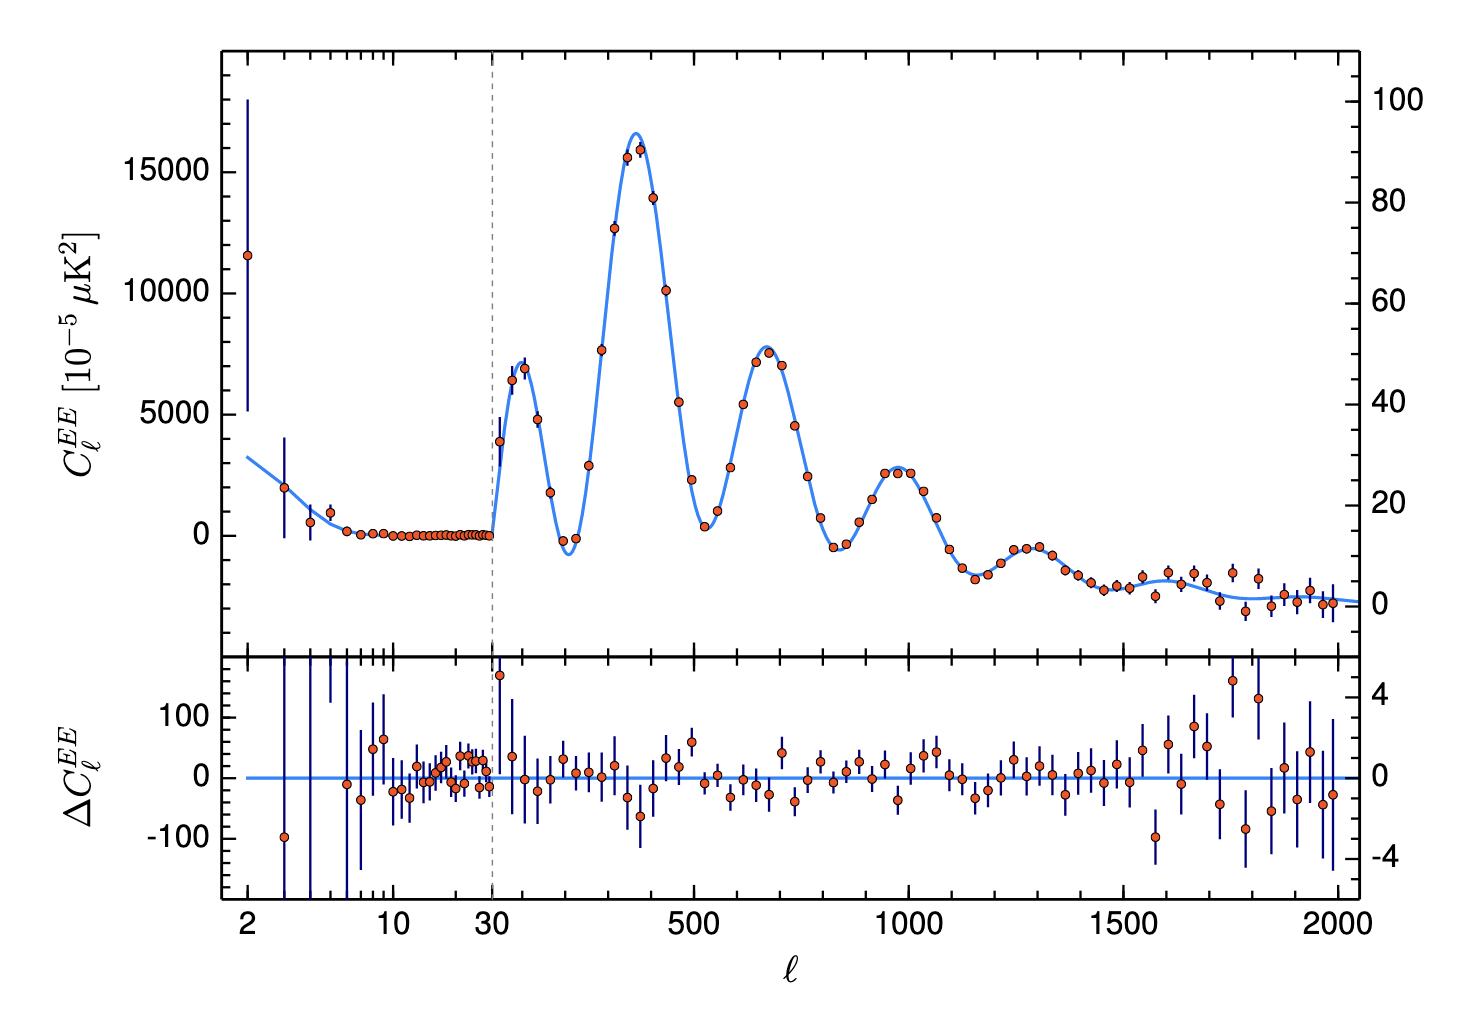
\includegraphics[width=12cm]{plots/planck_EE.png}
    \caption{Planck EE power spectrum}
    \label{fig:planck_ee}
\end{figure}
The other two power spectra are shown in figures~\ref{fig:planck_te} and~\ref{fig:planck_ee}. The main consideration with these two power spectra is to observe the way it breaks the degeneracy between $\tau_\mathrm{rei}$ and $\mathcal{A}_s,n_s$. In the TT case,  $\tau_{\mathrm{rei}}$ suppresses the power spectrum as it suppresses the fraction of light that reaches an observer. However, the additional scattering actual causes anisotropies in the polarization power spectrum to increase. Thus, the effects of $\mathcal{A}_s$ and $\tau_\mathrm{rei}$ are similar in the TT power spectrum but opposite in the $EE$ power spectrum. Thus, one needs all 3 power spectra to reliably infer the cosmological parameters.
\section{Tensions Between Weak Lensing and the CMB}
As seen, there are a total of five parameters needed to describe $\Lambda$CDM in weak lensing: $\Omega_m$, $\Omega_b$, $H_0$, $\mathcal{A}_s$, and $n_s$. This parameterization is not unique. Another common parameter, which tracks $\mathcal{A_s}$, is $\sigma_8$
\begin{equation}
	\sigma_8^2 = \left.\int\limits_0^\infty P(k,r)\left(\frac{3j_1(kr)}{kr}\right)^2\frac{k^2}{2\pi^2}dk\right|_{r=8}
\end{equation}
which can be described as the amplitude of matter fluctuations at the scale $8 h^{-1}\mathrm{Mpc}$. With this parameter instead of $\mathcal{A}_s$, weak lensing gives string constraints on $S_8 = \sigma_8\sqrt{\Omega_m/0.3}$. 

The reality is, however, that CMB measurements of some of these parameters differ between the parameters measured from weak lensing (precise results can be found in~\cite{amon_dark_2022,noauthor_planck_2018}). The most famous discrepancy is the $H_0$ tension (figure~\ref{fig:h0_tension}). Weak lensing measurements are significantly higher than CMB measurements; a nearly $5\sigma$ difference. The other famous tension is the $S_8$ tension at about a $3\sigma$ difference (figure~\ref{fig:s8_tension}). There have been extensive efforts to propose a model that can resolve these tensions (modified gravity, early dark energy, quintessence, etc.), but as of now no model can simultaneously resolve both tensions. For example, early dark energy resolves the $H_0$ tension, but the $S_8$ tension tends to either remain the same or increase. The remaining chapters will explore how to compute these tensions and demonstrate a proposed consistency test.
\begin{figure}[ht]
	\centering
	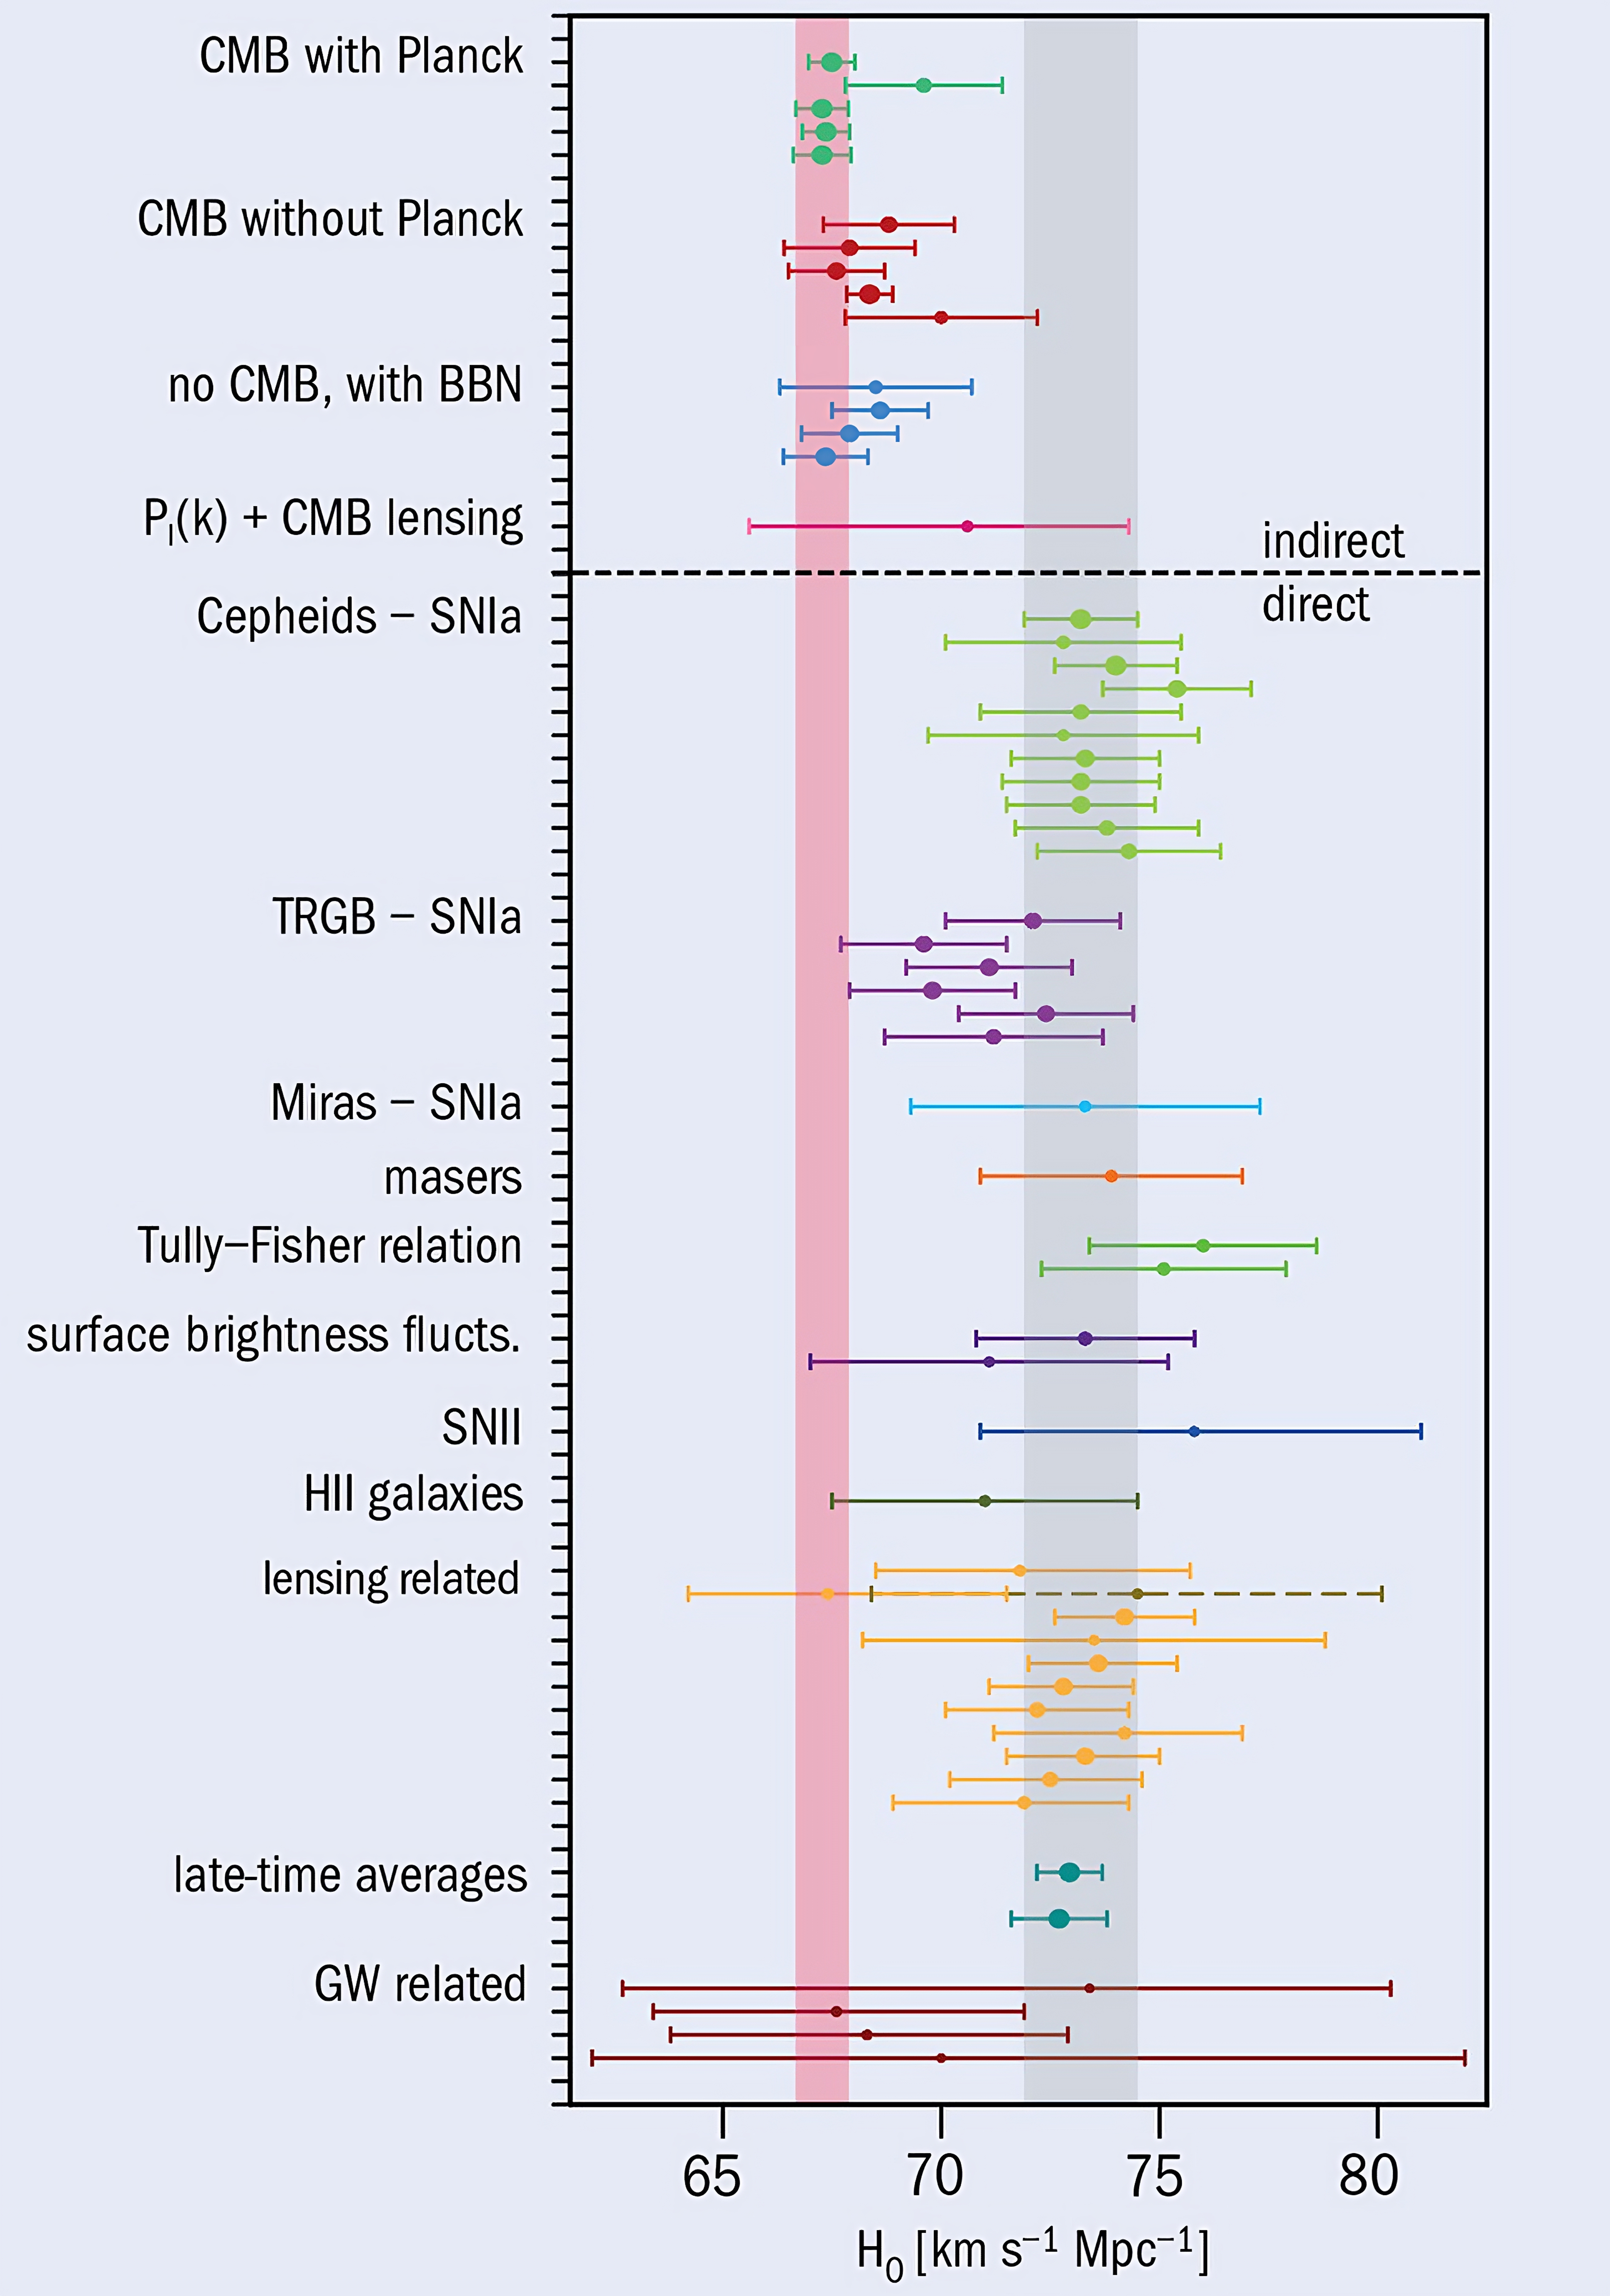
\includegraphics[width=0.75\textwidth]{plots/h0_tension_4x.jpeg}
	\caption{Measurements of $H_0$ from different experiments.}
	\label{fig:h0_tension}
\end{figure}
\begin{figure}[ht]
	\centering
	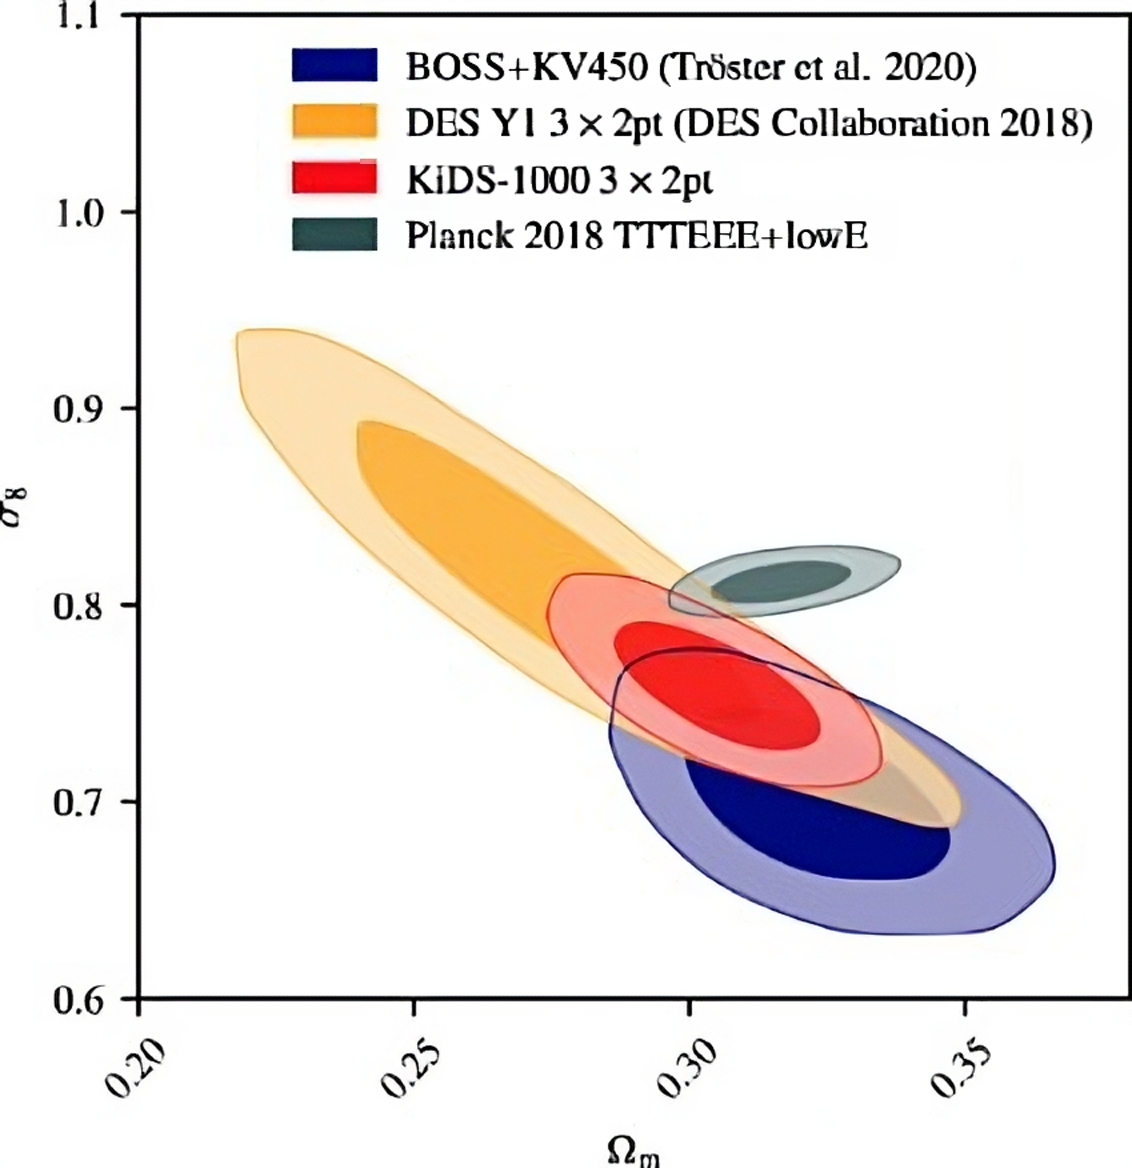
\includegraphics[width=0.75\textwidth]{plots/s8_tension_4x.jpeg}
	\caption{Measurements of $S_8$ from different experiments.}
	\label{fig:s8_tension}
\end{figure}









\chapter{Tension}
H0 and S8 tension
\section{Tension Metrics}

In a previous DES paper, the tension metrics are the following:
\begin{enumerate}
    \item Bayesian evidence ratio given by
	\[ R = \frac{\mathcal{E}_{AB}}{\mathcal{E}_A\mathcal{E}_B} \]
	Where $A$ and $B$ are data sets. This method can be written many ways using bayes theorem, which will make it appearent that this metric depends heavily on the prior volume.
    \item Bayesian suspiciousness. This metric attempts to remove the dependence on the prior volume by defining the suspiciousness as 
	\[ \log S = \log R - \log I \]
	Of particular interest here is the new value $I$ which is the information ratio, which is defined in terms of the KL divergence.
	\[ \log I = \mathcal{D}_A + \mathcal{D}_B - \mathcal{D}_{AB} \]
	\[ \mathcal{D} = \int \mathcal{P} \log(\frac{\mathcal{P}}{\Pi}) \]
    \item The method of parameter difference $\Delta$ and $n_\sigma$.
    \item Parameter difference in update form. Suppose you have two data sets $A$ and $B$. The idea is to look at the difference in mean and covariance between data set $A$ and data set $A+B$.
	\[Q_{\mathrm{UDM}} = {(\mu_A - \mu_{A+B})}^T{(C_A-C_{A+B})}^{-1}(\mu_A - \mu_{A+B}) \]
	$Q_{\mathrm{UDM}}$ will be $\chi^2$ distributed with $\rank(C_A-C_{A+B})$ degrees of freedom.
    \item Goodness of fit degredation. This is similar to the previous, where it looks at how the goodness of fit of the model in data set $A$ degrades after adding data set $B$. We have
	\[ Q_{\mathrm{DMAP}} = 2\mathcal{L}_{A}(\hat{\theta}_A) + 2\mathcal{L}_B(\hat\theta_B) - 2 \mathcal{L}_{A+B}(\hat\theta_{A+B}) \]
	with $\hat{\theta}$ being the parameter vector that maximizes the posterior, the maximum a posteriori. Again $Q_{\mathrm{DMAP}}$ is $\chi^2$ distributed. 
\end{enumerate}

\subsubsection{Metric 1: Parameter Difference}
The idea behind this metric is simple: if two data sets largely agree, there difference posterior will be centered at 0, so the integral will be close to 0.
To actually compute the integral we use the normalizing flow to learn the posterior and perform MCMC inegration. The integration error is determined using the Clopper-Pearson interval on the binomial distribution.

\subsubsection{Metric 2: Eigentension}
This metric is interesting.
We start by diagonalizing the covariance matrix on one of our data sets.
Then we take the ratio of the variance in the prior to the variance in the posterior and apply an ad hoc cut to determine which eigenmodes are well-measured.
The idea is that we should not include poorly measured eigenmodes in our tension analysis because the difference is dominated by the prior rather than the data itself.
Lastly we project the other data set onto the eigenmodes and perform the parameter difference metric on only the well-measured eigenmodes.

(here is a good place to compare with metric 1)

\subsubsection{Metric 3: Parameter Difference in Update Form}
As discussed above, we can compute the parameter $Q_{\mathrm{UDM}}$ by
\begin{equation}
    Q_{\mathrm{UDM}} = {(\mu_A - \mu_{A+B})}^T{(C_A-C_{A+B})}^{-1}(\mu_A - \mu_{A+B}) 
\end{equation}
The difference of means is precisely the mean of the parameter difference distribution, and we are using the covariance $C_A+C_{A+B}$.
Thus it is clear $Q_{\mathrm{UDM}}$ is $\chi^2$ distributed with degrees of freedom given by $\rank(C_A-C_{A+B})$. 
It is clear, however, that this metric relies on the parameter difference to be gaussian distributed because of its reliance on $Q_{\mathrm{UDM}}$ being $\chi^2$ distributed. Despite this, we proceed anyway. With proper calibration this metric can be useful even for non-gaussian posteriors.

\subsubsection{Metric 4: Goodness of Fit Degradation}

\subsubsection{Interpreting the Results}

Given some probability $P$ of a parameter shift, the following formula can give you the number of standard deviations if the probability shift comes from a gaussian distribution
\[ n_\sigma = \sqrt{2} \text{Erf}^{-1}(P) \]
I have a notebook using two unit gaussian priors separated by a distance $a$. This example can be computed analytically.
\begin{equation*}
    \begin{split}
	\mathcal{P}(\Delta \theta) &= \frac{1}{2\pi} \int\limits_{-\infty}^{\infty} e^{-\theta^2/2} e^{-{(\theta-\Delta\theta)}^2/2}  d\theta \\
				   &= \frac{1}{2\pi} \cdot \sqrt{\pi} e^{-{(\Delta\theta)}^2/4}\\
				   &= \frac{1}{\sqrt{4\pi}}e^{-{(\Delta\theta)}^2/4}\\
    \end{split}
\end{equation*}
The parameter difference posterior is a gaussian with standard deviation $\sqrt{2}$. The separation is fixed by $a$, hence the shift is $\mathcal{P}(a)$. Hence the shift probability is
\[ \Delta = \int\limits_{-a}^{a} e^{-{(\Delta\theta)}^2/4} d\Delta\theta \]
Lets use the example $a=2$. Then $n_\sigma = 2/\sqrt{2} = \sqrt{2}$. Using this we can work backwards to find $\Delta$ from a $z$-table to find $\Delta = 0.9207 - 0.0793 = 0.8414 $. 

\subsection{DES v Planck Results}
\subsection{Building from previous results}
\section{Computing techniques}
\subsection{MCMC}

Interestingly, MCMC algorithms have heavy analogies with statistical mechanics which are useful to demonstrate the concept. To examine this, lets first define what a Markov Chain is.
\begin{defn}
A sequence $X_1,\hdots,X_n$ of random elements is a \textit{Markov Chain} if the conditional distribution $X_{n+1}$ depends only on $X_n$. The set in which $X_i$ take values is called the \textit{state space} of the chain.
\end{defn}


\subsubsection{The Metropolis-Hastings Algorithm}
Suppose we want to sample from a distribution $p(x)$. $p(x)$ can be high dimensional and is generally difficult to calculate (evidence is hard to compute since it requires integration over the entire parameter space). The goal is to use Markov Chains to sample from $p(x)$ without needing to compute the evidence. This will be represented as a path through state space until the chain reaches a stable point (stationary state).

We start with a proposal distribution $g(x_n)$. Sample from the proposal distribution to find the next state $x_{n+1}$ with probability $g(x_{n+1}|x_n)$. This transition from state $n$ to state $n+1$ must follow the \textit{detailed balance condition}
\[ p(x_n) g(x_{n+1}|x_n) A(x_n \rightarrow x_{n+1}) = p(x_{n+1}) g(x_n|x_{n+1}) A(x_{n+1} \rightarrow x_{n}) \]
where $A$ is an \textit{acceptance probability} which I will define more precisely later. Using Bayes' Theorem on $p(x)$, the evidence cancels out on each side, and thus the detailed balance condition can be simplified to only rely on the likelihood and prior of $p(x)$, which I will denote $\pi$ and $\mathcal{L}$.
\[ \pi(x_n)\mathcal{L}(x_n) g(x_{n+1}|x_n) A(x_n \rightarrow x_{n+1}) = \pi(x_{n+1}) \mathcal{L}(x_{n+1}) g(x_{n}|x_{n+1}) A(x_{n+1}\rightarrow x_{n}) \]
\[ \Rightarrow \frac{A(x_n \rightarrow x_{n+1})}{A(x_{n+1}\rightarrow x_{n})} = \frac{\pi(x_{n+1}) \mathcal{L}(x_{n+1}) g(x_{n}|x_{n+1})}{\pi(x_n)\mathcal{L}(x_n) g(x_{n+1}|x_n)} \equiv R_{n,n+1} \]
This allows us to define the acceptance probability as
\[ A(x_n \rightarrow x_{n+1}) = \min( 1, R_{n,n+1} ) \]
This probability is used to determine whether the chain moves to $x_{n+1}$ or stays at $x_n$. The chain converges when it reaches a stationary state.

There are a few properties that can be observed for this algorithm:
\begin{itemize}
    \item Having an asymmetrical proposal $g(x)$ can allow for faster convergence of the chain.
    \item The initial sampling may not accurately reflect samples for $p(x)$. This is regarded as the `burn-in' and is generally discarded from the samples.
    \item MCMC Sampling loses sampling power for multi-modal distributions. 
\end{itemize}

\subsection{Data Emulators}

Traditional methods of computing likelihoods (e.g. \textsc{cosmosis}) require an immense number of CPU hours, and since we need tens of thousands of chains, we cannot rely on these traditional methods. To accelerate likelihood computation, and thus the MCMC process, we employ emulators which are neural networks that map the cosmological parameters to data vectors. The map is highly non-linear and thus a straightforward analytic mapping is not known. The neural network architecture used is similar for each experiment.

\subsubsection{LSST Emulator}
Unfourtunatly, we do not have access to the training samples for this emulator. We can however approximate the training region. First, we must define what tempered MCMC means. As discuss in the previous section, an MCMC decides wheather to accept or reject a point based on the detailed balance condition. In our case, we want to ensure the training samples cover a wide range in the parameter space, so we can modify the posterior by raising it to a power $T$ called the tempering factor. The detailed balance condition becomes

\[ \frac{A(x_n \rightarrow x_{n+1})}{A(x_{n+1}\rightarrow x_{n})} = \left[\frac{\pi(x_{n+1}) \mathcal{L}(x_{n+1})}{\pi(x_n)\mathcal{L}(x_n)}\right]^T \frac{ g(x_{n}|x_{n+1}) }{ g(x_{n+1}|x_n)} \]

It is believed the samples were generated via MCMC with a posterior tempering of $0.5$. This gives us the following distribution

\subsubsection{Planck $C_\ell$ Emulator}

Fortunately the training samples for \textsc{cosmopower} are available for download from google drive.

\subsection{Normalizing Flows}

The method of normalizing flows (MAF) implemented here uses Masked Autoencoders (MADE) to construct the flow. Suppose we have an input to the flow $x_i$. The output of the map is $y_i= \mu(x_{1:i-1})+\sigma(x_{1:i-1})x_i$. The $\mu$ and $\sigma$ are found using neural networks which recieve masked inputs $x_{1:i-1}=(x_1,\ldots,x_{i-1},0,\ldots,0)$. Since the input only depends on the first $i-1$ inputs, the normalizing flow is \textit{autoregressive} and the Jacobian is triangular.

The implementation in tensorflow uses \textit{bijectors} which implements a local diffeomorphism between a manifold $M$ and a target manifold $N$ (which are our parameter spaces), i.e. $\phi:M\rightarrow N$ such that $\phi$ is differentiable and injective. In tensorflow it has three operations, Forward, Inverse, and log\_deg\_jacobian, which are exactly the three we want. By constructing a bijector for each masked input, the full normalizing map can be constructed.

To give a motivation, I will begin with a 2 dimensional example. In this example I used \textsc{cobaya} to generate samples from two distributions. One is a pure gaussian centered at $(1/2,1/2)$ with covariance $0.005 I$  ($I$ is the identity matrix). The other is a circle of radius 1 with points generated by a gaussian based on its distance from the circle. In other words, it is a gaussian centered at $x^2+y^2$ with a mean of $x^2+y^2=1$ and a standard deviation $0.02$.

The first step is to find the parater difference distribution. Wrap the samples in the shorter chain until it is the same length as the longer chain, then take the difference of the two chains. In this example we get the following.

Now we can do the normalizing flow. As a general rule-of-thumb, the network will consist $2d$ MAfs each of $2$ hidden layers with $2d$ hidden units each, with $d$ the dimension of the distribution.
This will generally give an expressive model without introducing error from the inability to train all of the models parameters in a reasonable time. 
These parameters are tunable to whatever the user will decide, and some experimentation with these parameters is needed to ensure the best results.
In addition, we allow the parameters to be arbitrarily permuted between each MAF since the resulting probability of shift should be independent of parameterization.

One advantage of normalizing flows is its effectiveness for smaller data sets. (talk about NF vs KDE when the data is available).
\chapter{Growth-Geometry Split in DES-Y3}
Parameter splitting is a common method used to attempt to resolve the tensions discussed in the previous chapter. The idea is to split a parameter and choose analysis settings that restrict each split parameter to describe specific cosmological effects. One of these splits is a growth-geometry split, where we split the relative matter density $\Omega_m$ and the dark energy equation of state $w$ into two parameters. The growth parameter is designed to describe the late-time growth of structure and the geometry parameter designed to describe the background evolution. After splitting the parameters, one can do an analysis to determine how the tension changes and if the split parameters have distinct values from each other. This chapter describes the growth geometry split in $\Omega_m$ and $w$ in DES-Y1~\cite{muir_y1_2021} and DES-Y3. These results are also available in a paper written by Kunhao Zhong, another Masters student, and myself, on arXiv~\cite{zhong_growth_2023} and are pending publication in Physical Review.
\section{Split Matter Power Spectrum}
Since the matter density $\Omega_m$ is split into two parameters, $\Omega_m^{\text{growth}}$ and $\Omega_m^{\text{geo}}$, a single growth factor and a single matter power spectrum; these are split as well. From equation 2.8, the linear matter power spectrum is proportional to the square of the linear growth factor $D_+(z(a)) = G(z)/(1+z)$, so the growth and geometry power spectra are related by
\begin{equation}
	P^L_{\text{split}}(k,z) = P^L_{\text{geo}}(k,z) \left(\frac{G_{\text{growth}}(z)}{G_{\text{geo}}(z)}\right)^2
\end{equation}
which means $\sigma_8$ is also split according to
\begin{equation}
	\sigma_{8,\text{split}}^2 = \sigma_{8,\text{geo}}^2 \left(\frac{G_{\text{growth}}(z)}{G_{\text{geo}}(z)}\right)^2
\end{equation}
In this analysis, however, we want to go beyond linear scales. To achieve this, we use the Euclid Emulator to emulate the non-linear matter power spectrum by computing a boost factor
\begin{equation}
	P(k,z) = P^L(k,z) \times B(k,z)
\end{equation}
\begin{figure}[ht]
	\centering
	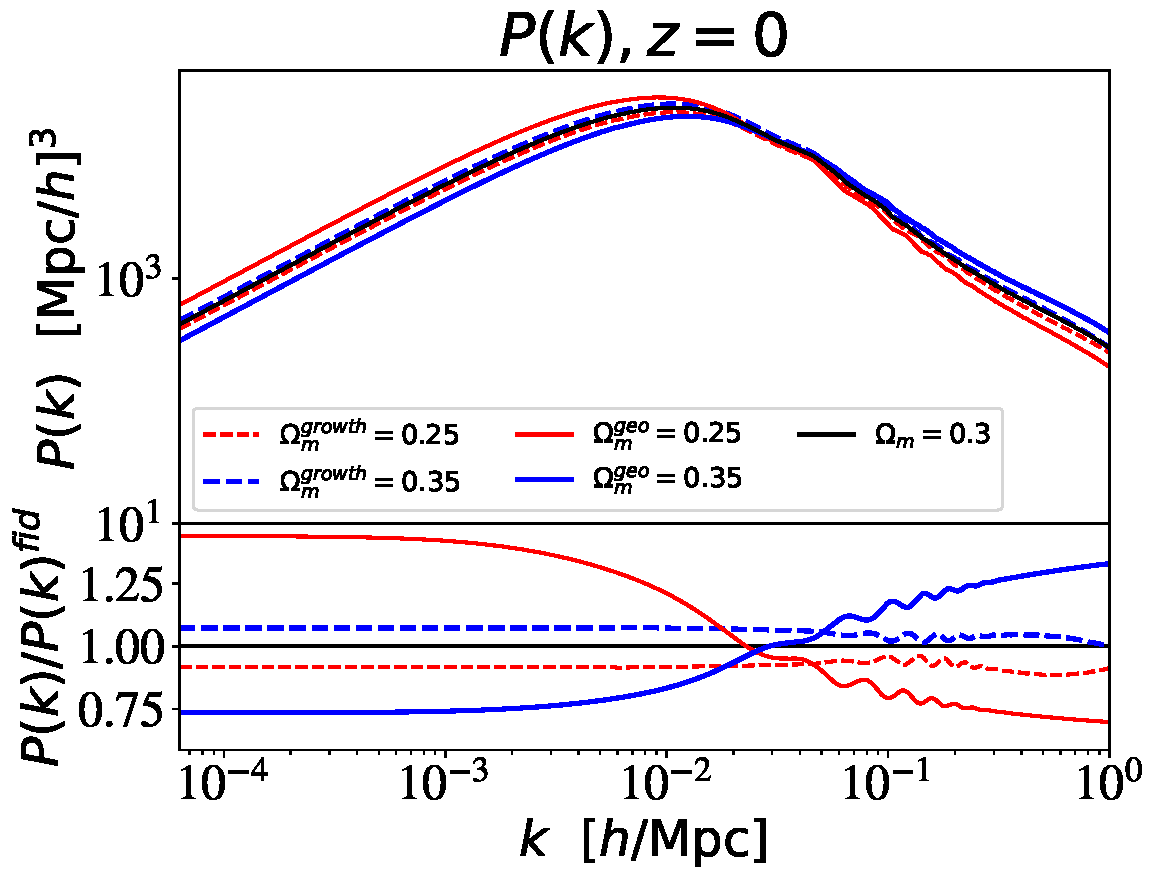
\includegraphics[width=0.75\textwidth]{plots/Pk.pdf}
	\caption{Non-linear power spectrum from Euclid emulator. When either the geometry or growth parameters are varied, the other is kept fixed at $\Omega^X=0.3$.}
	\label{fig:pk}
\end{figure}
While the growth parameters are scale-independent, there is a crossing for the geometry parameters. This is due to the enhanced gravitational effects for higher $\Omega_m^{\mathrm{geo}}$, or suppressed gravitational effects for lower $\Omega_m^\mathrm{geo}$. From this, one can predict that the value of $\sigma_8$ will change, the change being larger for $\Omega_m^\mathrm{geo}$ than $\Omega_m^\mathrm{growth}$, and increases in either $\Omega_m$ will increase $\sigma_8$. We see this is true in figure~\ref{fig:sigma8_l}
\begin{figure}[ht]
	\centering
	\begin{subfigure}[b]{0.49\textwidth}
		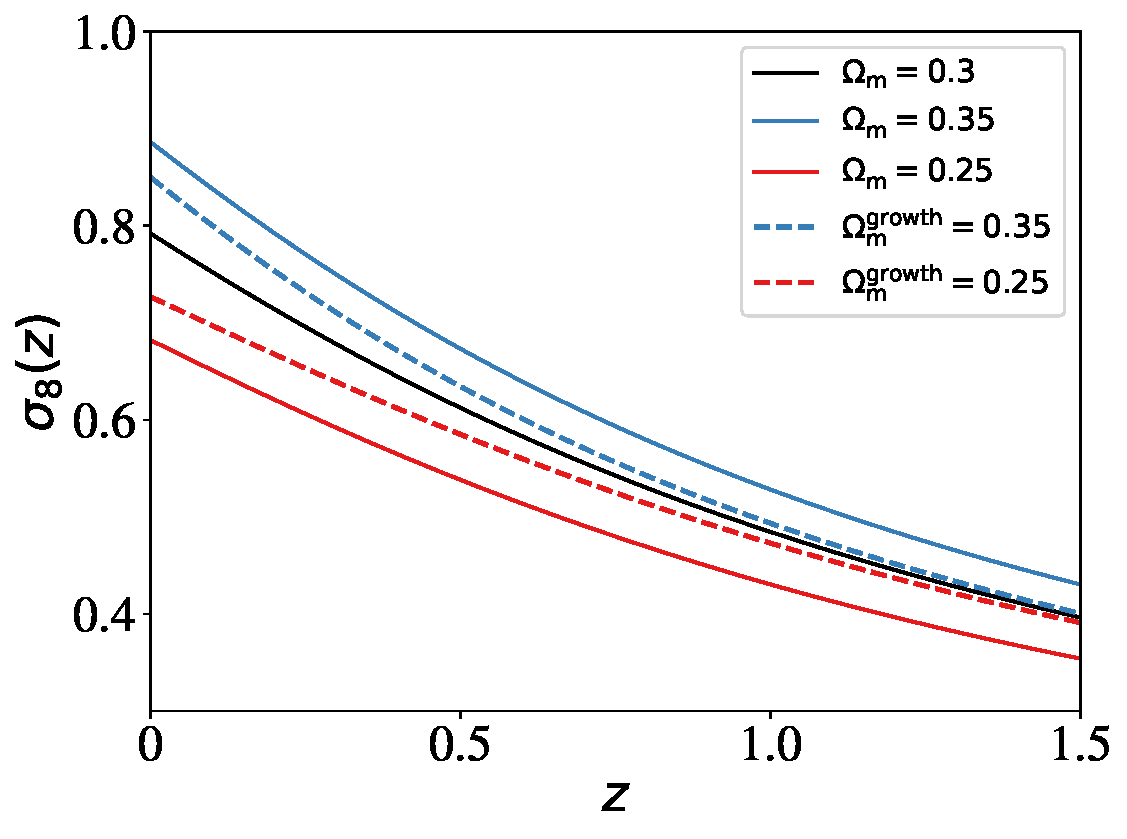
\includegraphics[width=\textwidth]{plots/sigma8.pdf}
		\caption{$\Lambda$CDM split.}
		\label{fig:sigma8_l}
	\end{subfigure}
	\begin{subfigure}[b]{0.49\textwidth}
		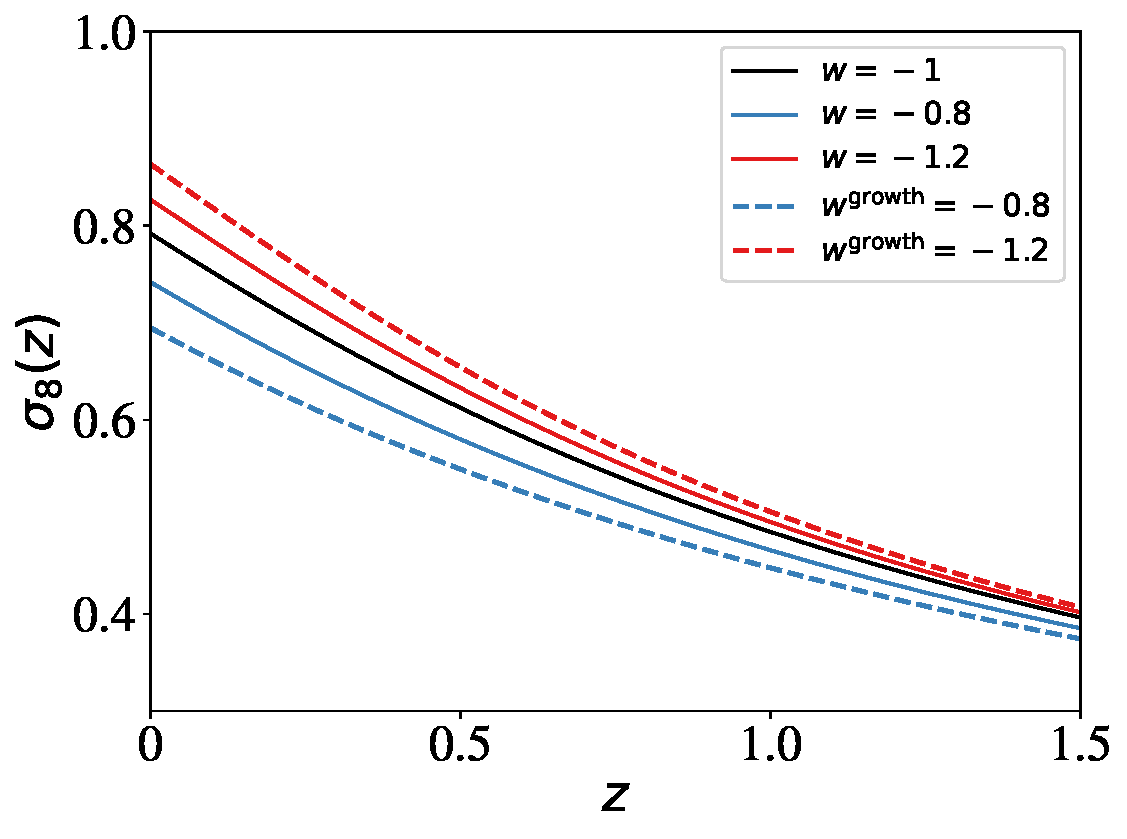
\includegraphics[width=\textwidth]{plots/sigma8_w.pdf}
		\caption{$w$CDM split.}
		\label{fig:sigma8_w}
	\end{subfigure}
	\label{fig:sigma8}
	\caption{Effect of changing growth and geometry parameters on $\sigma_8(z)$.}
\end{figure}
One surprising feature of figure~\ref{fig:sigma8_w} is that these effects are the opposite. However, this result is not surprising. Increasing $w$, where $w<0$, coincides with decreasing the pressure or increasing density.
\section{Data and Analysis Pipeline}
\subsection{DES Parameter Priors}
This analysis is done on data from the Dark Energy Survey (DES), both year 1 (Y1) and year 3 (Y3), combined with CMB data. The cosmological parameters of interest and their priors are given in table~\ref{table:cosmo_prior}.
\begin{table}
\centering
\begin{tabular}{lr}
	\hline
	Parameter & Prior \\
	\hline\hline
	$\Omega_m^{\text{geo}}$    & $\mathcal{U}(0.1,0.9)$   \\
	$w^{\mathrm{geo}}$         & $\mathcal{U}(-3,-0.01)$  \\
	$\mathcal{A}_s\times10^9$  & $\mathcal{U}(1.7,2.5)$   \\
	$n_s$                      & $\mathcal{U}(0.92,1.0)$  \\
	$H_0$                      & $\mathcal{U}(61,73)$     \\
	$\tau$                     & $\mathcal{U}(0.01,0.8)$  \\
	$\Omega_m^{\text{growth}}$ & $\mathcal{U}(0.24,0.4)$  \\
	$w^{\mathrm{growth}}$      & $\mathcal{U}(-1.7,-0.7)$ \\
	\hline
\end{tabular}
\caption{Summary of cosmological parameters and their priors.}
\label{table:cosmo_prior}
\end{table}
The priors on ($\Omega_m^{\text{geo}}$, $w^{\mathrm{geo}}$, $\mathcal{A}_s\times10^9$, $n_s$, $H_0$) are taken from the Euclid Emulator prior. $\tau$ is only included in chains that also contain CMB data.
\begin{table}
\centering
\begin{tabular}{lcc} % 
\hline
DES Systematics Parameter &  Y1 Prior & Y3 Prior \\
\hline\hline
\textbf{Linear Galaxy bias} \\
$ b_g^i(i \in [1,5])$ & Flat(0.8, 3.0) & Flat(0.8, 3.0)\\
\hline
\textbf{Intrinsic Alignment (NLA)} \\
$A_{1}$ &  Flat(-5, 5) & \\
$A_{2}$ &  Flat(-5, 5) & \\
\hline
\textbf{Intrinsic Alignment (TATT)} \\
$A_{1}$    & & Flat(-5, 5) \\
$A_{2}$    & & Flat(-5, 5) \\
$\eta_{1}$ & & Flat(-5, 5) \\
$\eta_{2}$ & & Flat(-5, 5) \\
$b_{TA}$   & & Flat(0, 2) \\
\hline
\textbf{Source photo-z} \\
$\Delta z_{\mathrm{s}}^{1} \times 10^{2}$ & Gauss(-0.1, 1.6)  & Gauss(0, 1.8) \\
$\Delta z_{\mathrm{s}}^{2} \times 10^{2}$ & Gauss(-0.19, 1.3) & Gauss(0, 1.5) \\
$\Delta z_{\mathrm{s}}^{3} \times 10^{2}$ & Gauss(0.9, 1.1)   & Gauss(0, 1.1)\\
$\Delta z_{\mathrm{s}}^{4} \times 10^{2}$ & Gauss(-1.8, 2.2)  & Gauss(0, 1.7)\\
\hline
\textbf{Lens photo-z}\\
$\Delta z_{\mathrm{1}}^{1} \times 10^{2}$ & Gauss(0.8, 0.7)  & Gauss(0.6, 0.4)  \\
$\Delta z_{\mathrm{1}}^{2} \times 10^{2}$ & Gauss(-0.5, 0.7) & Gauss(0.1, 0.3)  \\
$\Delta z_{\mathrm{1}}^{3} \times 10^{2}$ & Gauss(0.6, 0.6)  & Gauss(0.4, 0.3)\\
$\Delta z_{\mathrm{1}}^{4} \times 10^{2}$ & Gauss(0, 0.01)   & Gauss(-0.2, 0.5)\\
$\Delta z_{\mathrm{1}}^{5} \times 10^{2}$ & Gauss(0, 0.01)  & Gauss(-0.7, 0.1)\\
\hline
\textbf{Multiplicative shear calibration} \\
$m_{1} \times 10^2$ & Gauss(1.2, 2.3) & Gauss(-0.6, 0.9)\\
$m_{2} \times 10^2$ & Gauss(1.2, 2.3) & Gauss(-2.0, 0.8)\\
$m_{3} \times 10^2$ & Gauss(1.2, 2.3) & Gauss(-2.4, 0.8)\\
$m_{4} \times 10^2$ & Gauss(1.2, 2.3) & Gauss(-3.7, 0.8)\\
\hline
\textbf{Lens magnification} \\
$C_{\mathrm{1}}^1 \times 10^2$ & & Fixed (0.63)\\
$C_{\mathrm{1}}^2 \times 10^2$ & & Fixed (-3.04)\\
$C_{\mathrm{1}}^3 \times 10^2$ & & Fixed (-1.33)\\
$C_{\mathrm{1}}^4 \times 10^2$ & & Fixed (2.50)\\
$C_{\mathrm{1}}^5 \times 10^2$ & & Fixed (1.93)\\
\hline
\textbf{Point mass marginalization} \\
$B_i(i \in [1,5])$ & & Flat(-5, 5) \\
\hline
\end{tabular}
\caption{Summary of Priors on DES-Y1 and DES-Y3 systematics parameters.}
\label{table:prior_choices}
\end{table}
The external data sets used are
\begin{itemize}
	\item CMBP: The Planck CMB TTTEEE power spectra together with the non-linear low-$\ell$ EE power spectrum. The spectra are truncated after the first peak ($35<\ell<396$). This mitigates CMB lensing effects, which affect small-scale anisotropies. It also minimizes the late time Integrated Sachs Wolfe effect, which also has a larger effect on small scales.
	\item SNIa: Pantheon Type Ia supernova. As a distance probe, this prior constrains geometry parameters. There are growth effects that we choose not to model at this point, namely the peculiar velocity distributions of supernovae.
	\item BBN: We use a derived constraint on $100\Omega_bh^2$ from Big Bang Nucleosynthesis as
	\item BAO: BAO data is taken from the SDSS DR7 main galaxy sample, the 6dF galaxy survey, and the combined SDSS BOSS DR12 low-$z$ and CMASS galaxy samples. Again, as a distance probe, this is taken as geometry information.
\end{itemize}
To understand these choices of priors, we consider the following combinations:
\begin{itemize}
	\item Prior 1 (P1): Emulator prior + CMBP
	\item Prior 2 (P2): Emulator prior + SNIa + BBN + BAO
	\item Prior 3 (ALL): Emulator prior + CMBP + SNIa + BBN + BAO
\end{itemize}
\subsection{Software Pipeline}
To compute the linear matter power spectrum, we use \textsc{CAMB} Boltzmann code, which is capable of solving the linear Boltzmann equation and computing transfer functions. For going beyond linear scales, we use the Euclid emulator, a fast neural network-based emulator for Halofit. Previous DES studies used Halofit itself, a full N-body simulation, to determine the non-linear evolution of dark matter. A baseline comparison between the Euclid emulator and Halofit was done (figure~\ref{fig:euc_v_halo})
\begin{figure}[ht]
	\centering
	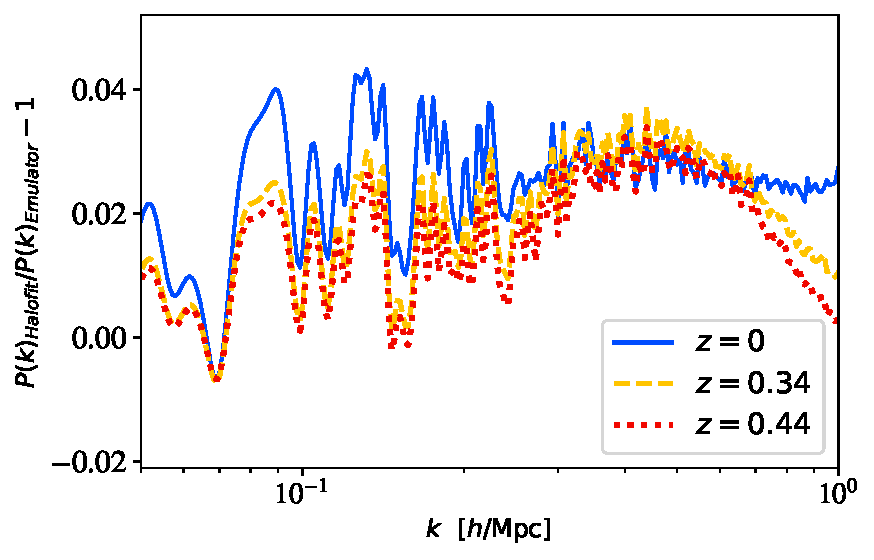
\includegraphics[width=0.75\textwidth]{plots/halo_vs_emu.pdf}
	\caption{Relative difference between Euclid emulator and Halofit.}
	\label{fig:euc_v_halo}
\end{figure}
We use the Cocoa (CObaya-COsmolike joint Architecture). This interfaces Cobaya, the MCMC sampler we use, with CosmoLike, the data vector calculation framework. DES-Y3 has already been implemented in Cobaya, CosmoLike, and Cocoa. To assess the convergence of the MCMC, we use the $R-1<0.02$.

One benefit of this analysis is that growth parameters are semi-fast; they do not require CAMB to recompute the matter power spectrum, they only require CosmoLike to update the data vectors. Rerunning CosmoLike with only changing the growth parameters results in a 2-fold speedup.
\subsection{Pipeline Validation on Synthetic Data}
To validate this method, we generate a synthetic data vector at the Planck best-fit parameters without lensing (equation~\ref{eq:planck_best_fit}), and we hope to find no difference between growth and geometry parameters and hope each parameter is equal to the fiducial value.
\begin{equation}\label{eq:planck_best_fit}
	(\mathcal{A}_s\times10^{-9}, n_s, H_0, \Omega_m, \Omega_b) = (2.101,0.965,67.32,0.317,0.049)
\end{equation}
Using the ALL prior and external data, there is marginal improvement between the cosmic shear constraints on $\Omega_m^\mathrm{growth}$ compared to the prior. However, there is significant improvement in the $3\times2$pt case compared to cosmic shear. 

In $w$CDM, there is poor constraining power on $\Omega_m^\mathrm{growth}$ and $w^{\mathrm{growth}}$, even with the most informative $3\times2$pt case. For this case, we give constraining power along the first principal component
\begin{equation}
	\mathrm{PC}_1 \equiv 0.7071\Delta\Omega_m - 0.7071\Delta w\,.
\end{equation}
In all 3 sets of priors and external data, and despite the inclusion of additional nuisance parameters from the TATT model, we find similar constraining power on $\Omega_m^\mathrm{growth}$ between DES-Y1 and DES-Y3. In the $3\times2$pt case with the ALL prior gives a smaller ($\sim17\%$) error bar. Constraints on $\mathrm{PC}_1$ are prior dominated and nearly identical for the $w$CDM split in DES-Y1 and DES-Y3.
\begin{figure}[ht]
	\centering
	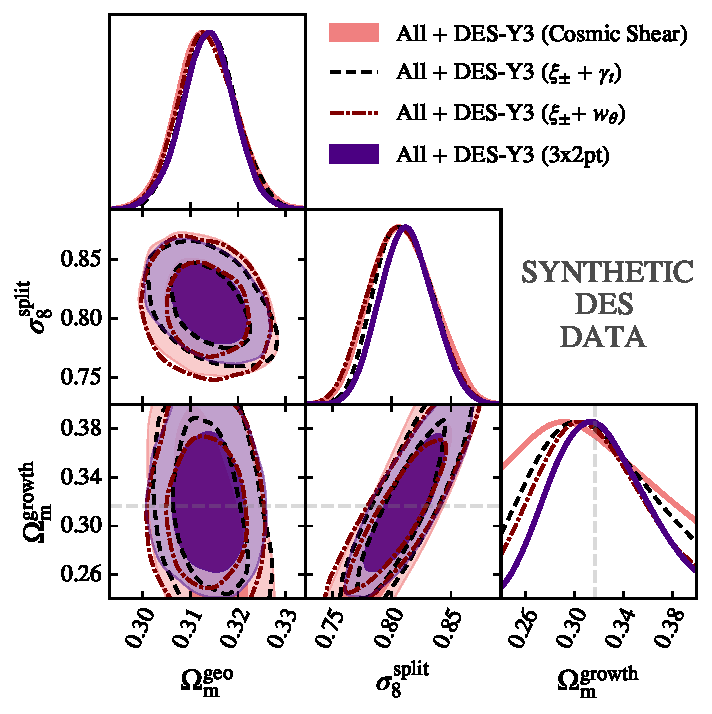
\includegraphics[width=0.75\textwidth]{plots/plot36_S8.pdf}
	\caption{Cosmic shear, $2\times2$pt combinations, and $3\times2$pt posteriors for DES-Y3 with the ALL prior.}
	\label{fig:syn_y3_probe}
\end{figure}
\begin{figure}[ht]
	\centering
	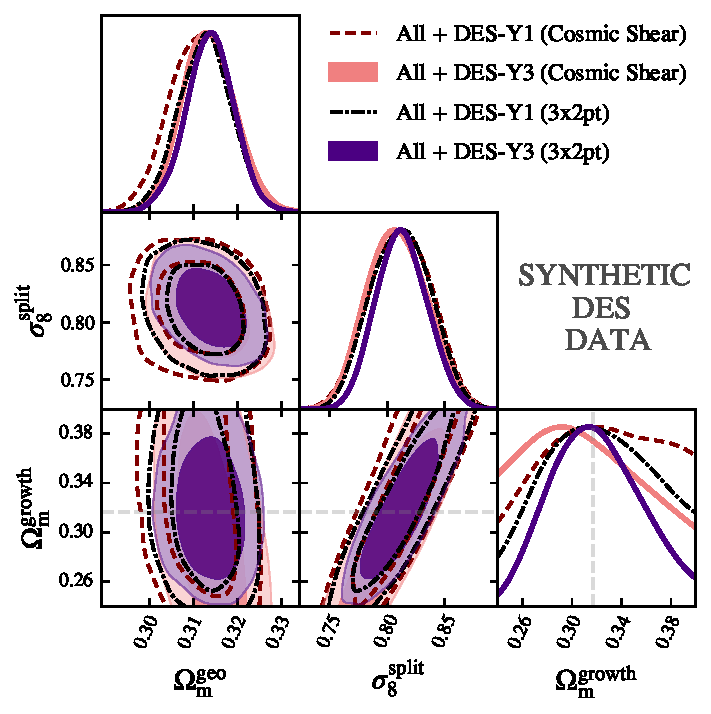
\includegraphics[width=0.75\textwidth]{plots/plot31v3.pdf}
	\caption{Comparison of DES-Y1 and DES-Y3 posteriors.}
	\label{fig:syn_y1_y3}
\end{figure}
\section{Results}
\subsection{\texorpdfstring{$\Lambda\text{CDM}$}{LCDM}}
For the most constraining case, $3\times2$pt with all prior, there is no evidence of a difference between $\Omega_m$ growth and geometry parameters (figure~\ref{fig:y3_3x2_all}). Exploring this further, however, we can look at various 2-point correlation functions is DES-Y1 and DES-Y3 (figure~\ref{fig:y3_2x2}). We see a significant change in the DES-Y3 cosmic shear-galaxy clustering posterior and the galaxy lensing-galaxy clustering posterior. However, these shifts from $\Delta\Omega_m=0$ are prior dominated, not data dominated, thus do not constitute evidence for a shift.
\begin{figure}[ht]
	\centering
	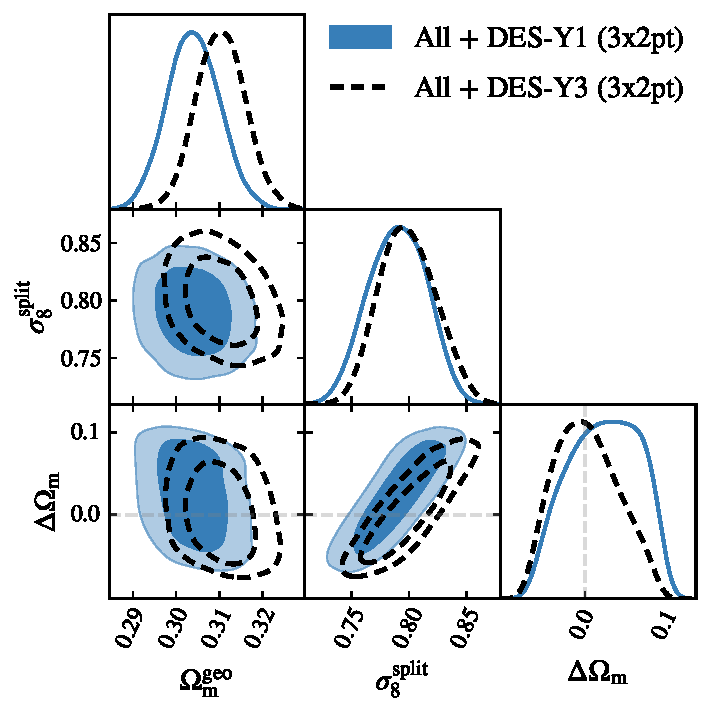
\includegraphics[width=0.75\textwidth]{plots/plot204_v2.pdf}
	\caption{Split posteriors for DES-Y3 $3\times2$pt and ALL prior.}
	\label{fig:y3_3x2_all}
\end{figure}
\begin{figure}[ht]
	\centering
	\begin{subfigure}[b]{0.45\textwidth}
		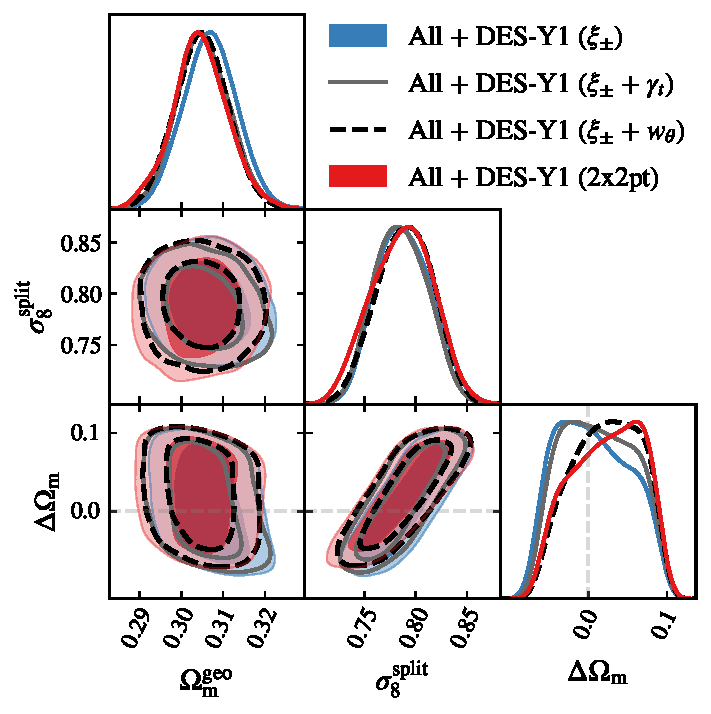
\includegraphics[width=\textwidth]{plots/plot208_v3.pdf}
		\caption{DES-Y1}
		\label{fig:y1_2x2_lcdm}
	\end{subfigure}
	\begin{subfigure}[b]{0.45\textwidth}
		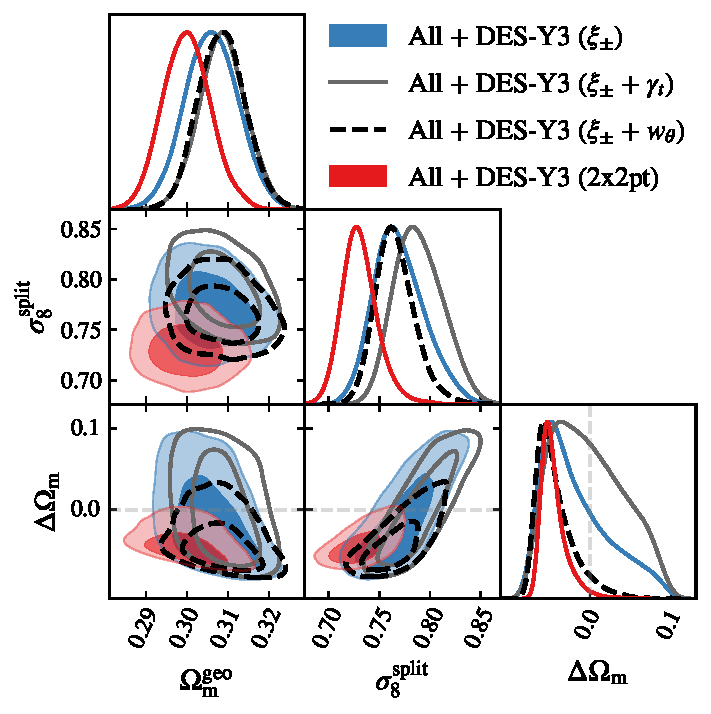
\includegraphics[width=\textwidth]{plots/plot208_v2.pdf}
		\caption{DES-Y3}
		\label{fig:y3_2x2_lcdm}
	\end{subfigure}
	\caption{DES-Y1 and DES-Y3 posteriors for 2-point correlation functions.}
	\label{fig:y3_2x2}
\end{figure}
The full results of the 1d marginalizations with each choice of prior is summarized in figure~\ref{fig:lcdm_result_1d}. Aside from the 2-point correlation functions, every $\Delta\Omega_m$ result is compatible with 0 to within 1-sigma.
\begin{figure}[ht]
	\centering
	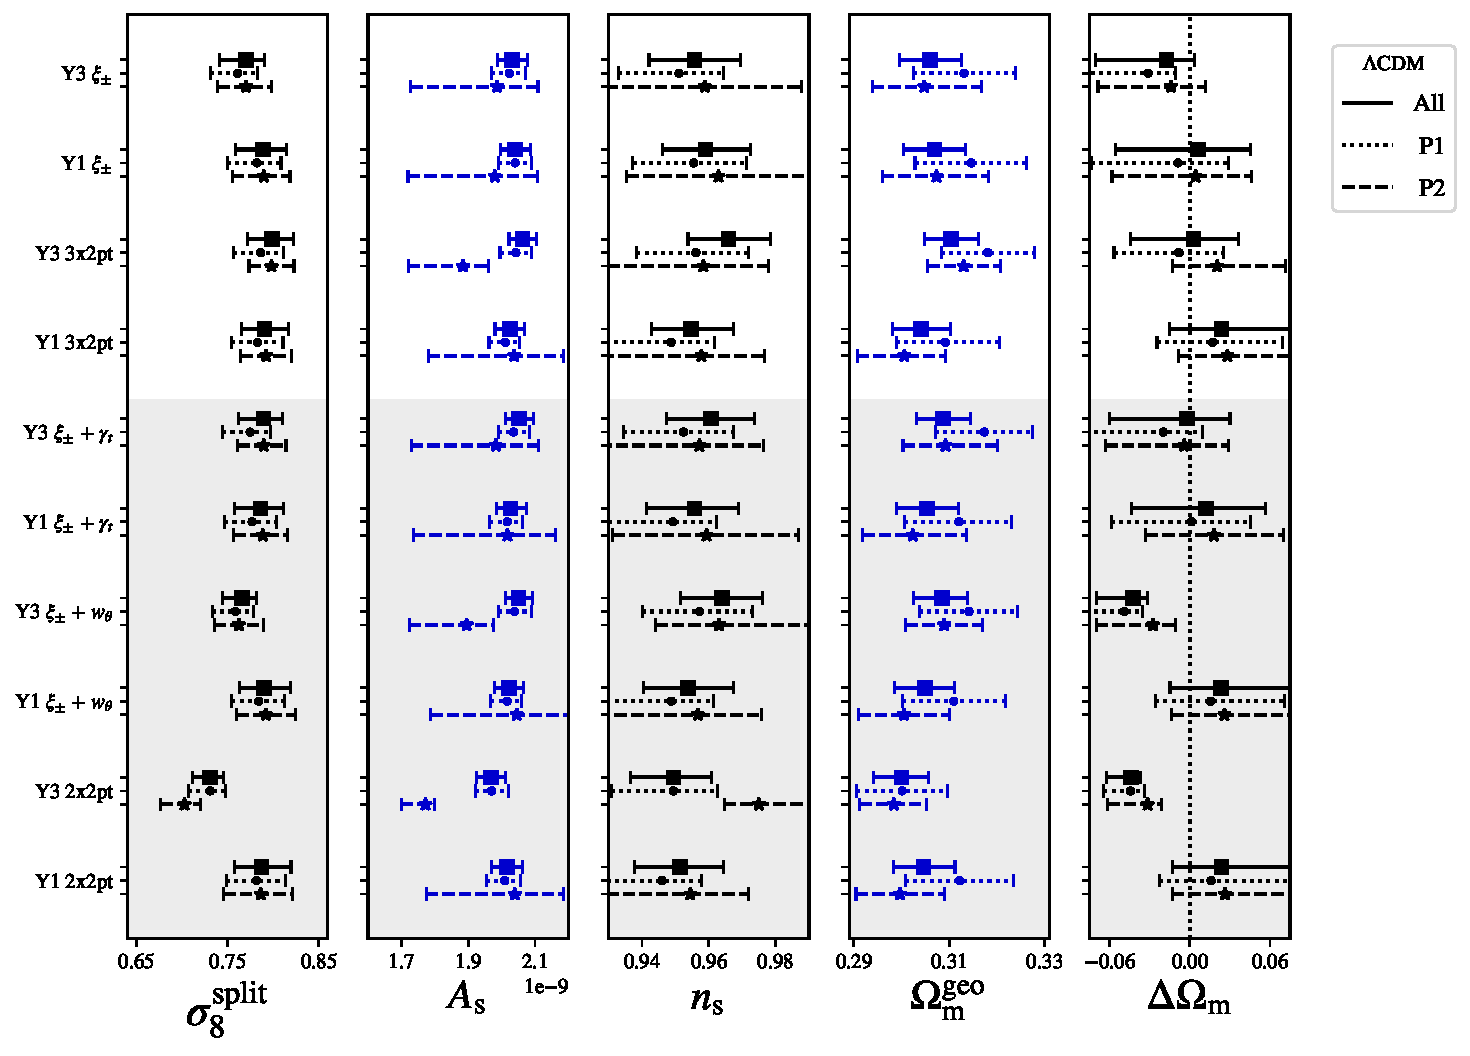
\includegraphics[width=\textwidth]{plots/plot_1d_resultv5.pdf}
	\caption{Full 1d results for $\Lambda$CDM split}
	\label{fig:lcdm_result_1d}
\end{figure}
Similarly to the synthetic chains, the $3\times2$pt data chains with ALL prior have improved constraining power on $\Delta\Omega_m$ in DES-Y3 over DES-Y1. However, the improvement is around 10\%, slightly less than the 17\% observed in the synthetic data. 

The mentioned 2-point correlation functions that do have significant shifts in $\Omega_m$ are determined to be at $1.75\sigma$ for the cosmic shear-galaxy clustering and $2.60\sigma$ for galaxy clustering-galaxy-galaxy lensing. Because of known inconsistencies in the RedMaGiC galaxy samples, these are not attributed to discovery.
\subsection{\texorpdfstring{$w$CDM}{wCDM}}
The results for $w$CDM are summarized in figures~\ref{fig:wcdm_post} and~\ref{fig:wcdm_result_1d}. Again, there is no evidence of a shift in $\mathrm{PC}_1$ from 0. The exception is, once again, the DES-Y3 $2\times2$pt with ALL prior. The significance of the shift is $4.48\sigma$. Again, this shift may be attributed to the RedMaGiC. 
\begin{figure}[ht]
	\centering
	\begin{subfigure}[b]{0.45\textwidth}
		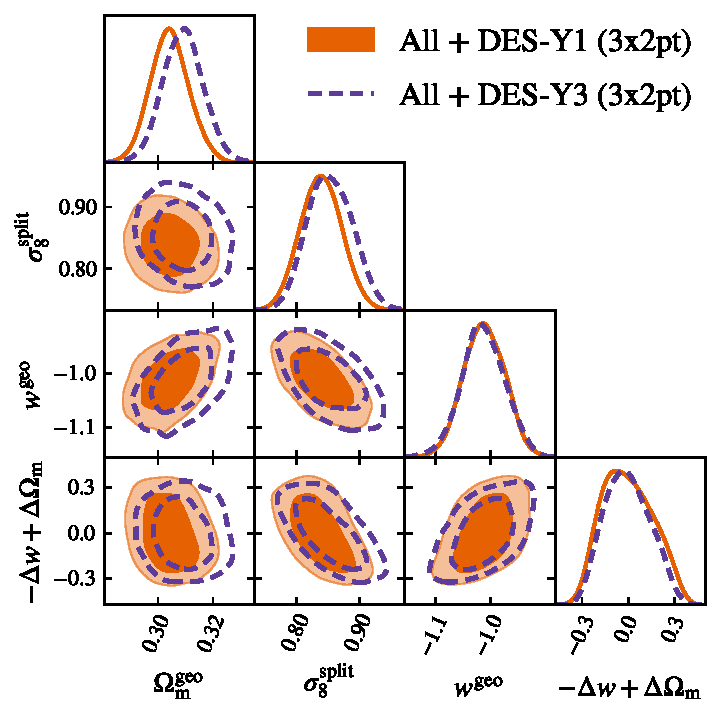
\includegraphics[width=\textwidth]{plots/plot205v2.pdf}
		\caption{DES-Y1 vs. DES-Y3 $3\times2$pt $w$CDM posteriors.}
		\label{fig:y3_y1_wcdm}
	\end{subfigure}
	\begin{subfigure}[b]{0.45\textwidth}
		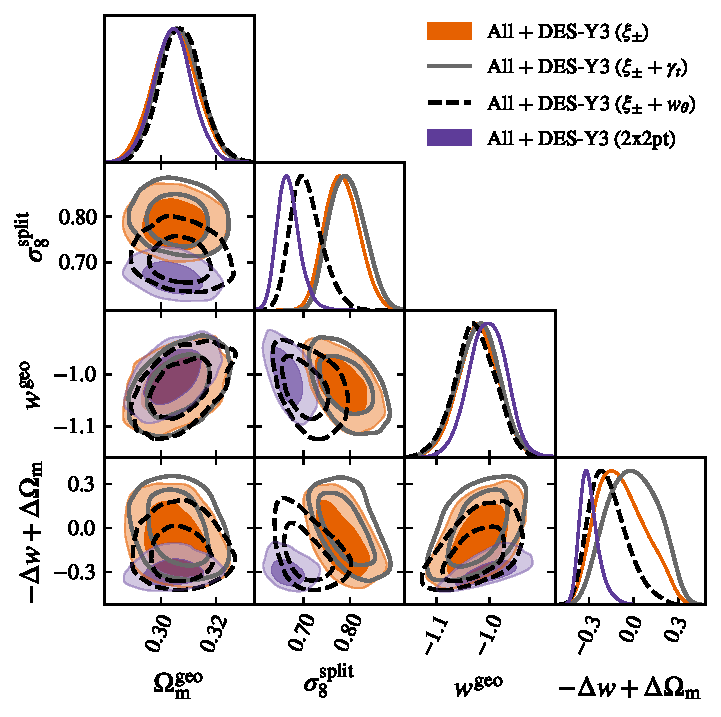
\includegraphics[width=\textwidth]{plots/plot209.pdf}
		\caption{DES-Y3 2-point correlation function posteriors}
		\label{fig:y3_2x2_wcdm}
	\end{subfigure}
	\caption{$w$CDM posteriors.}
	\label{fig:wcdm_post}
\end{figure}
\begin{figure}[ht]
	\centering
	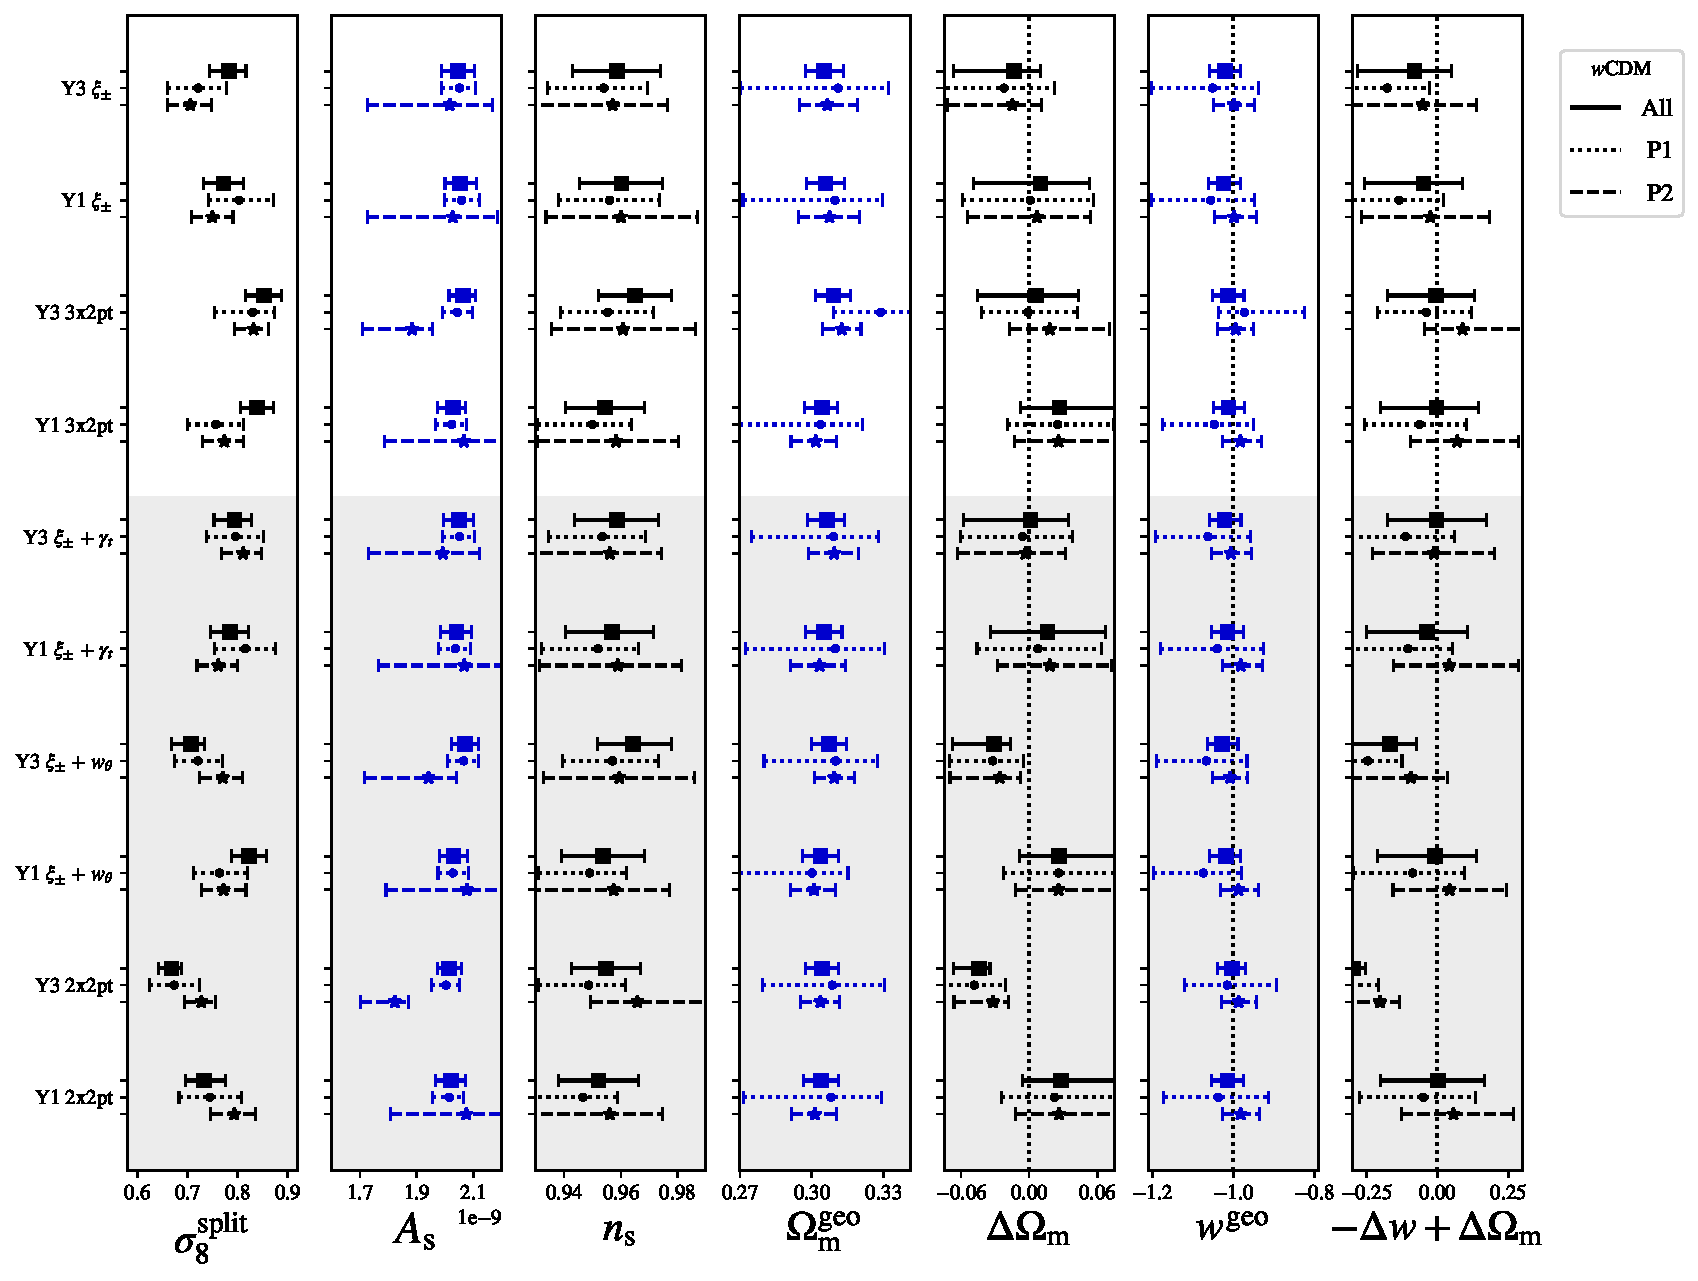
\includegraphics[width=\textwidth]{plots/plot_1d_resultv6.pdf}
	\caption{Full 1d results for $\Lambda$CDM split}
	\label{fig:wcdm_result_1d}
\end{figure}
\subsection{Tension Analysis}
We conclude by testing the internal consistency between the Y1 and Y3 data sets independently. This is done using the parameter difference method, where we use normalizing flows to learn the posterior distribution. The results are summarized in figure~\ref{fig:tension}. The tension is computed with the parameters $(\mathcal{A}_s,n_s,H_0,\Omega_m^{\mathrm{geo}},\sigma_8^\mathrm{split})$ (with $w^{\mathrm{geo}}$ added in the $w$CDM case). Interestingly, the tension appears to be generated predominantly by $\mathcal{A}_s$. Additionally, the $2\times2$pt correlation functions have a significant degradation in the goodness of fit when CMB priors are added. This reflects the RedMaGiC inconsistency discussed above. A study allowing $X_\mathrm{lens}$ to vary is required to analyze this shift fully.

In the $w$CDM case, we once again see the $2\times2$pt has a significant shift. Contrary to the split $\Lambda$CDM case, the $\mathcal{A}_s$ tension is much smaller, making the detection of a shift in $\mathrm{PC}_1$ more meaningful. Once again, an analysis involving $X_\mathrm{lens}$ is required to assess the source of this detection.
\begin{figure}[ht]
	\centering
	\begin{subfigure}[b]{0.45\textwidth}
		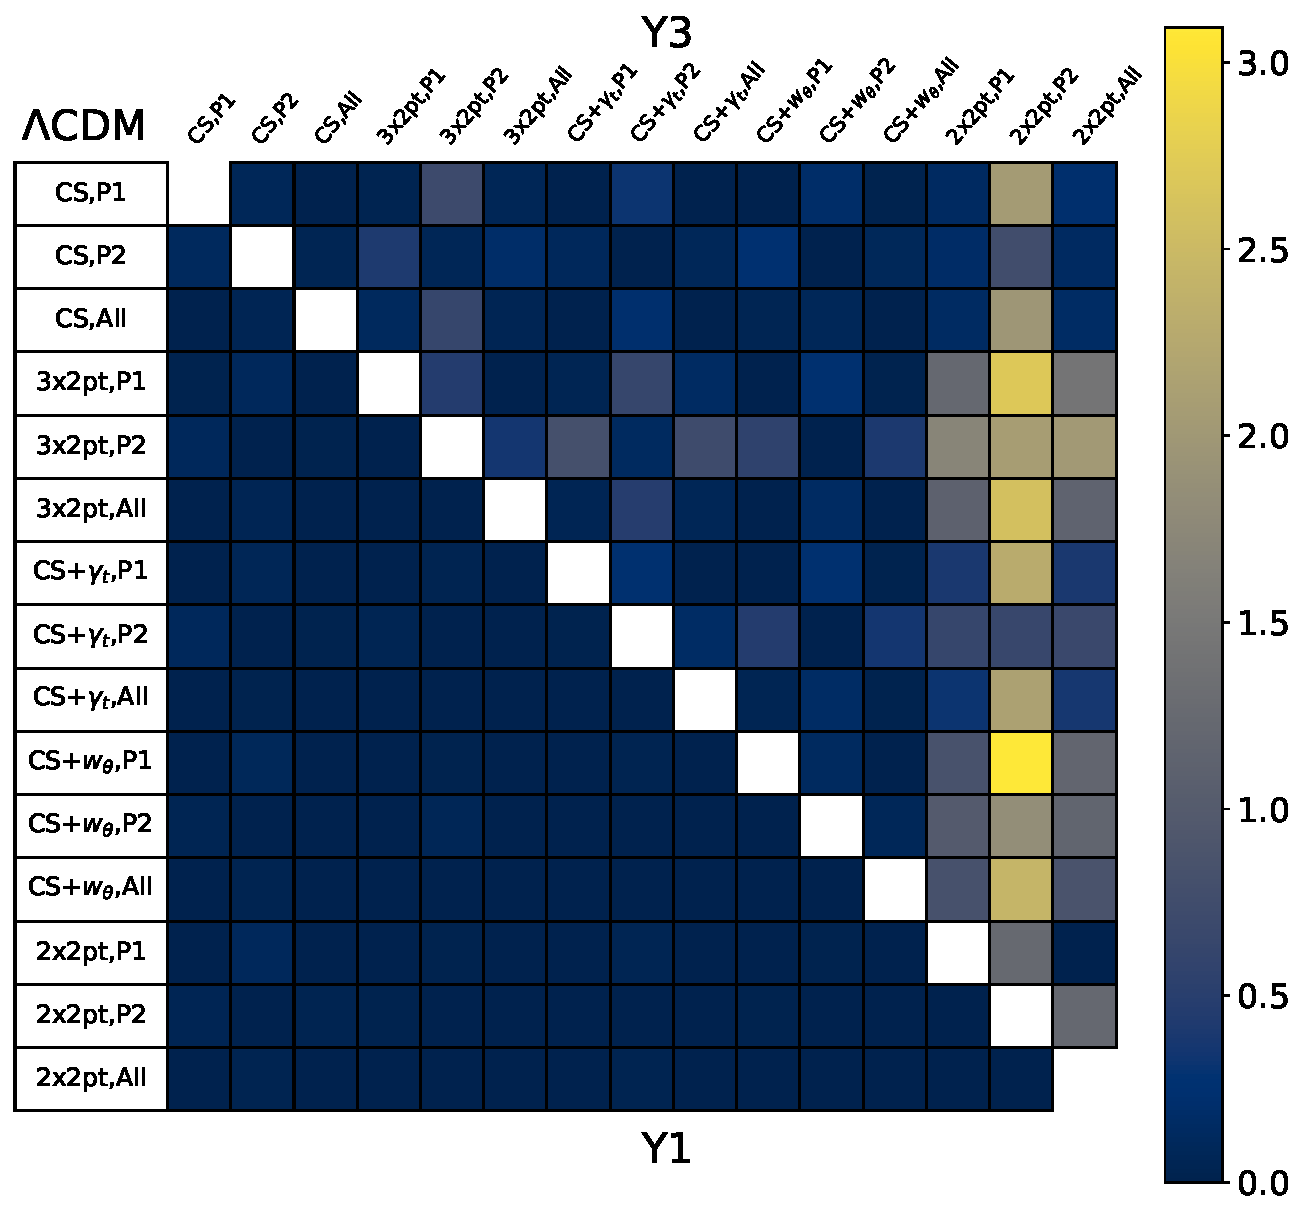
\includegraphics[width=\textwidth]{plots/internal_tension_v4.pdf}
		\caption{Internal tension in the $\Lambda$CDM split.}
		\label{fig:lcdm_tension}
	\end{subfigure}
	\begin{subfigure}[b]{0.45\textwidth}
		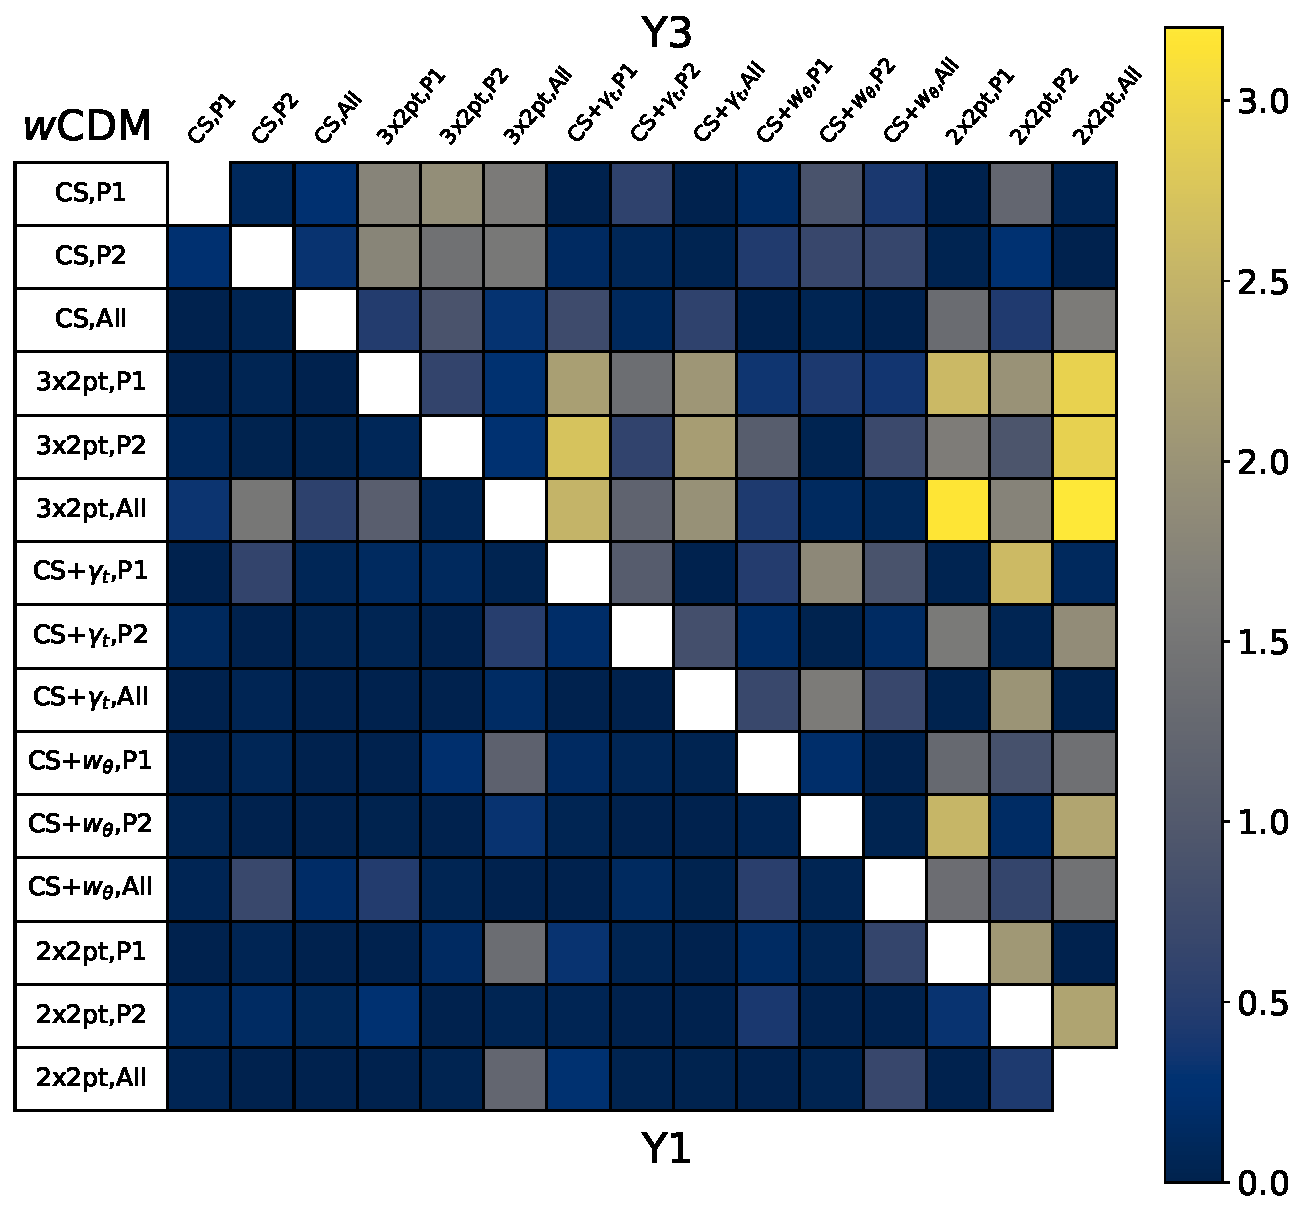
\includegraphics[width=\textwidth]{plots/internal_tension_wcdm.pdf}
		\caption{Internal tension in the $w$CDM split}
		\label{fig:wcdm_tension}
	\end{subfigure}
	\caption{}
	\label{fig:tension}
\end{figure}
\section{Conclusion}
We split $\Omega_m$ and $w$ into two parameters, one governing the background evolution and the other governing the late-time scale-independent growth of structure. We consider DES data together with various external data sets and priors from the CMB, supernovae, BBN, and BAO. We then run MCMC on DES-Y1 and DES-Y3 data and evaluate the difference between the growth and geometry parameters. 

As demonstrated, there is little evidence of a difference between growth and geometry parameters in DES-Y1 and DES-Y3. The exception is the $2\times2$pt chains, however, there is an internal inconsistency with the RedMaGiC samples that may source this result. Because we fixed $X_\mathrm{lens}=1$, an additional analysis can be done investigating if $X_{\mathrm{lens}}$ can source a significant shift. Additionally, one can repeat the analysis with the MagLim lensing samples. In the future, additional datasets from Rubin Observatory's LSST, the Euclid mission, Dark Energy Spectroscopic Instrument, Simons Observatory, and CMB-S4 can be used to improve the constraints derived in this analysis

\chapter{Data Emulators}
As can be seen from the growth-geometry split analysis, a great amount of time and computing resources are needed to do a comprehensive analysis of novel cosmological models and extensions to $\Lambda$CDM. There are a growing number of proposed extension theories, and more data sets that can test them. One of the ways to improve the efficiency of data and theory analysis is to create a faster way to compute data vectors when doing MCMC sampling. In this chapter, I will describe how one can use neural networks (NN) to learn this mapping, bypassing the need for expensive programs such as Comsolike.
\section{Neural Networks}
Although the term `neural network' is almost synonymous with magic in the modern world, the concept is very natural from elementary mathematics. We start with the most basic example: linear regression. 

In linear regression, one considers a model of the form $y=mx+b$. The goal is to find the values of $m$ and $b$ that minimizes the square of the residual
\begin{equation}
	L(y_{i,\mathrm{truth}},y_{i,\mathrm{model}}) = (y_{i,\mathrm{truth}} - y_{i,\mathrm{model}})^2\,.
\end{equation}
In this very special case, there is an analytic way to minimize $L$, but in general that is highly non-trivial. Additionally, there are much more complicated data sets one would want to model, such as data vectors in cosmological surveys. The remaining question is: how does one intelligently generalize this type of model to more complicated ones?

We have a tool that can do this already: the brain~\cite{noauthor_what_nodate}! The brain is a large system of cells called neurons. Each neuron is connected to others by a synapse, and after accumulating a large enough electric charge, the neuron will activate, sending the electric signal to a connected neuron. 

Using this, lets try to construct a general model. We start with the neurons
\begin{figure}[th]
	\centering
	\begin{tikzpicture}
		\draw (-2,0) circle (5pt);
		\draw (0,0) circle (5pt);
		\draw (2,0) circle (5pt);
		\draw (1,1.41) circle (5pt);
		\draw (-1,1.41) circle (5pt);
		\draw (1,-1.41) circle (5pt);
		\draw (-1,-1.41) circle (5pt);
	\end{tikzpicture}
	\caption{Arrangement of neurons.}
	\label{fig:neurons}
\end{figure}
Now we add in the synapses, the connections between neurons. In general, not every neuron is connected to each other. It should be noted, along each synapse is an activation function. Rather than having a threshold potential like a real synapse, NNs use functions that represent the activation of the neuron. Also, each synapse has a weight that represents the strength of the connection.
\begin{figure}[th]
	\centering
	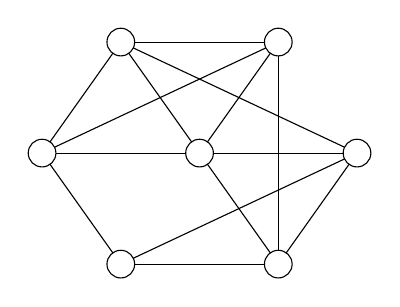
\begin{tikzpicture}
		\draw (-2,0) -- (0,0);
		\draw (-1,1.41) -- (0,0);
		\draw (-1,1.41) -- (-2,0);
		\draw (-1,-1.41) -- (-2,0);
		\draw (-1,-1.41) -- (1,-1.41);
		\draw (2,0) -- (1,-1.41);
		\draw (1,1.41) -- (-1,1.41);
		\draw (1,1.41) -- (1,-1.41);
		\draw (2,0) -- (-1,-1.41);
		\draw (0,0) -- (1,-1.41);
		\draw (0,0) -- (1,1.41);
		\draw (0,0) -- (2,0);
		\draw (-1,1.41) -- (2,0);
		\draw (1,1.41) -- (-2,0);
		\draw[fill=white] (-2,0) circle (5pt);
		\draw[fill=white] (0,0) circle (5pt);
		\draw[fill=white] (2,0) circle (5pt);
		\draw[fill=white] (1,1.41) circle (5pt);
		\draw[fill=white] (-1,1.41) circle (5pt);
		\draw[fill=white] (1,-1.41) circle (5pt);
		\draw[fill=white] (-1,-1.41) circle (5pt);
	\end{tikzpicture}
	\caption{Neurons with synapses.}
	\label{fig:neurons_synapse}
\end{figure}
Next, we define which neurons receive an external signal, and which give a signal to the outside. These act as our input and output.
\begin{figure}[th]
	\centering
	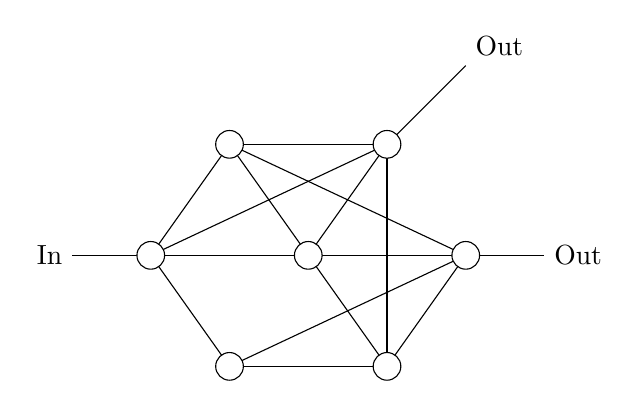
\begin{tikzpicture}
		\draw (-2,0) -- (0,0);
		\draw (-1,1.41) -- (0,0);
		\draw (-1,1.41) -- (-2,0);
		\draw (-1,-1.41) -- (-2,0);
		\draw (-1,-1.41) -- (1,-1.41);
		\draw (2,0) -- (1,-1.41);
		\draw (1,1.41) -- (-1,1.41);
		\draw (1,1.41) -- (1,-1.41);
		\draw (2,0) -- (-1,-1.41);
		\draw (0,0) -- (1,-1.41);
		\draw (0,0) -- (1,1.41);
		\draw (0,0) -- (2,0);
		\draw (-1,1.41) -- (2,0);
		\draw (1,1.41) -- (-2,0);
		\draw (-3,0) -- (-2,0);
		\draw (-3,0) node[anchor=east] {In};
		\draw (1,1.41) -- (2,2.41);
		\draw (2,0) -- (3,0);
		\draw (3,0) node[anchor=west] {Out};
		\draw (2,2.41) node[anchor=south west] {Out};
		\draw[fill=white] (-2,0) circle (5pt);
		\draw[fill=white] (0,0) circle (5pt);
		\draw[fill=white] (2,0) circle (5pt);
		\draw[fill=white] (1,1.41) circle (5pt);
		\draw[fill=white] (-1,1.41) circle (5pt);
		\draw[fill=white] (1,-1.41) circle (5pt);
		\draw[fill=white] (-1,-1.41) circle (5pt);
	\end{tikzpicture}
	\caption{Neurons, synapses, and IO.}
	\label{fig:neurons_synapse_io}
\end{figure}
Finally, we have a choice to make in the activation function. This is the chance to greatly increase the modelling capability of NNs. As we will see in the future, the only requirement is that the function is continuous, thus we can use non-linear activation functions, allowing modelling of highly non-linear outputs. The goal is to define a loss function that we want to minimize (in the linear regression, the loss is the square of the residual). The loss function is a function of the output of the NN, and the output is parameterized by the parameters of the NN. Thus, if $y=\phi(\alpha_i,x)$ represents the output of the neural network with parameters $\alpha_i$ and input $x$, the loss function is, in fact, parameterized by the neural network as well.
\begin{equation}
	L(y) = L(\phi(\alpha_i,x)) = \mathfrak{L}(\alpha_i,x)
\end{equation}
Thus, a neural network is, in simple terms, an optimization problem. The issue, however, is that neural networks generally have a large number of parameters (thousands, millions, even billions!), so this optimization is difficult in practice. Also, what may appear as a simple loss function in terms of the output can become an extremely complicated (and, importantly, non-monotonic) function of $\alpha_i$.

The general method of optimization is called \textit{gradient descent}. The strategy is the following:
\begin{enumerate}
	\item Define an initial set of parameters $\alpha_{i,\mathrm{init}}$.
	\item Split the training data into $n$ batches
	\item Generate a new set of parameters for each batch, centered around $\alpha_{i,\mathrm{init}}$, denoted $\alpha^{n}_{i}$.
	\item Compute the loss for each batch.
	\item Compute the gradient of the neural network.
	\item Update the parameters according to the gradient.
	\item Repeat until gradient is 0.
\end{enumerate}
This simple algorithm has one glaring flaw, it is prone to getting stuck in local minima. Ideally, we want to search for the global minimum for the loss function. The way around this is to add some stochasticity to the gradient descent so that the network does not simply search for zero gradient. Instead, the parameters are updated probabilistically from the gradient.

The gradient is usually computed using \textit{backpropagation}, in which the gradient is computed at each layer and the total gradient is computed according to the chain rule. This presents an issue: if the gradient is small at each layer, the gradient will be small on the order of $\epsilon^{n}$, where $n$ is the number of layers. This can lead to a misleading gradient that vanishes, or a gradient that explodes to large values. This is the problem of \textit{vanishing gradients}, and we will discuss ways to avoid this in the next section.

The last issue to mention is that, given a large number of parameters, it is possible to fit the training data very well, but the model is not able to fit external data sets. This is called \textit{overfitting}. There are many strategies to resolve this. The two we will use is dropout and L2 regularization. Dropout randomly sets a fraction of the weights to zero, meaning the NN will not be able to rely on individual neurons to get a reliable output. This ensures the full network is being used. L2 regularization penalizes the model for learning large weights, which again means the model relies on particular neurons. This is accomplished by modifying the loss function by adding the L2 norm of the network.
\begin{equation}
	L(y) \mapsto L(y)+\sum_i \alpha_i^2
\end{equation}
In summary, a NN is a directed graph, where each edge has a weight and an activation function, and each node has a value that it passes along to the edge. The inputs are propagated to the output, and the goal is to minimize the loss of the output. Its important to pick a smart loss function depending on one's needs from the NN and a smart activation function depending on the values of each node. The loss function is minimized using stochastic gradient descent. It is also important to implement strategies to avoid overfitting on the training data by penalizing the model for relying too heavily on certain regions of the graph.
\section{Architecture Choices}
As discussed before, the weights, activation functions, and connections are choices we can make for a neural network. Together, they comprise the architecture. In this section, we will discuss the architecture choices we have made.

Before discussing the graph architecture, we want to highlight the choice of activation function. Before giving any data to the neural network, we do some preprocessing to the data. The first thing we do is normalize the input and output. The input is the cosmological parameters, which we process each parameter to follow a normal distribution.
\begin{equation}
	x^i = \frac{\theta^i - \bar\theta^i}{\sigma_i}
\end{equation}
The output is the cosmic shear data vector. We preprocess this by diagonalizing and normalizing each component.
\begin{equation}
	y^i = \frac{ (P^{-1}d)^i }{\sqrt{(PCP^{-1})^{ii}}}
\end{equation}
Where $C$ is the covariance of the data and $P$ the change of basis matrix to the eigenbasis of $C$. This generally means we will have a lot of negative parameters, and the input and output are both symmetric about 0, thus we choose to use an antisymmetric activation function so that the symmetry around 0 can be preserved. In our case, we use $\tanh(x)$. Additionally, all of these NNs are feedforward sequential models. Sequential means we separate the neurons into layers, and feedforward means the data moves only from layer $n$ to layer $n+1$ and never backwards.
\subsection{Multi-Layer Perceptron}
The first graph architecture we study in the multi-layer perceptron (the name is adopted from convolutional neural networks `perceiving' image features). In this architecture, a node in a given layer is connected to every node in the following layer, so this network is called `simply connected' (figure~\ref{fig:mlp}).
\begin{figure}[ht]
	\centering
	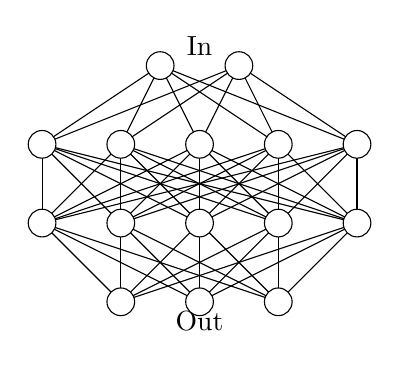
\begin{tikzpicture}
		\draw (0,2) node[anchor=south] {In};
		\draw (-0.5,2) -- (-2,1);
		\draw (-0.5,2) -- (-1,1);
		\draw (-0.5,2) -- (0,1);
		\draw (-0.5,2) -- (1,1);
		\draw (-0.5,2) -- (2,1);
		\draw (0.5,2) -- (-2,1);
		\draw (0.5,2) -- (-1,1);
		\draw (0.5,2) -- (0,1);
		\draw (0.5,2) -- (1,1);
		\draw (0.5,2) -- (2,1);
		%1-2
		\draw (-2,1) -- (-2,0);
		\draw (-2,1) -- (-1,0);
		\draw (-2,1) -- (0,0);
		\draw (-2,1) -- (1,0);
		\draw (-2,1) -- (2,0);
		\draw (-1,1) -- (-2,0);
		\draw (-1,1) -- (-1,0);
		\draw (-1,1) -- (0,0);
		\draw (-1,1) -- (1,0);
		\draw (-1,1) -- (2,0);
		\draw (0,1) -- (-2,0);
		\draw (0,1) -- (-1,0);
		\draw (0,1) -- (0,0);
		\draw (0,1) -- (1,0);
		\draw (0,1) -- (2,0);
		\draw (1,1) -- (-2,0);
		\draw (1,1) -- (-1,0);
		\draw (1,1) -- (0,0);
		\draw (1,1) -- (1,0);
		\draw (1,1) -- (2,0);
		\draw (2,1) -- (-2,0);
		\draw (2,1) -- (-1,0);
		\draw (2,1) -- (0,0);
		\draw (2,1) -- (1,0);
		\draw (2,1) -- (2,0);
		%2-3
		\draw (-2,0) -- (-1,-1);
		\draw (-2,0) -- (0,-1);
		\draw (-2,0) -- (1,-1);
		\draw (-1,0) -- (-1,-1);
		\draw (-1,0) -- (0,-1);
		\draw (-1,0) -- (1,-1);
		\draw (0,0) -- (-1,-1);
		\draw (0,0) -- (0,-1);
		\draw (0,0) -- (1,-1);
		\draw (1,0) -- (-1,-1);
		\draw (1,0) -- (0,-1);
		\draw (1,0) -- (1,-1);
		\draw (2,0) -- (-1,-1);
		\draw (2,0) -- (0,-1);
		\draw (2,0) -- (1,-1);
		\draw (0,-1) node[anchor=north] {Out};
		%layer in to 1
		\draw[fill=white] (-0.5,2) circle (5pt);
		\draw[fill=white] (0.5,2) circle (5pt);
		\draw[fill=white] (-2,1) circle (5pt);
		\draw[fill=white] (-1,1) circle (5pt);
		\draw[fill=white] (0,1) circle (5pt);
		\draw[fill=white] (1,1) circle (5pt);
		\draw[fill=white] (2,1) circle (5pt);
		\draw[fill=white] (-2,0) circle (5pt);
		\draw[fill=white] (-1,0) circle (5pt);
		\draw[fill=white] (0,0) circle (5pt);
		\draw[fill=white] (1,0) circle (5pt);
		\draw[fill=white] (2,0) circle (5pt);
		\draw[fill=white] (-1,-1) circle (5pt);
		\draw[fill=white] (0,-1) circle (5pt);
		\draw[fill=white] (1,-1) circle (5pt);
	\end{tikzpicture}
	\caption{A multi-layer perceptron.}
	\label{fig:mlp}
\end{figure}
\subsection{Residual Network}
As mentioned above, there is an issue of vanishing gradients with deep neural networks. To resolve this, one can add the input and output together so that gradient information is allowed to skip layers~\cite{he_deep_2015}(figure~\ref{fig:resblock}). Suppose we have a block of layers parameterized by $\alpha_i$, and its input is from another layer, parameterized by $\beta_i$, so that $w=\chi(\beta_i,x)$ for an input $x$. Then the block of layers, whose map is denoted $\phi$, will be
\begin{equation}
	\phi(\alpha_i,\chi(\beta_i,x)) = \psi(\alpha_i,\beta_i,x)+\chi(\beta_i,x)
\end{equation}
This section of the model is going to attempt to learn
\begin{equation}
	\psi(\alpha_i,\beta_i,x)-\chi(\beta_i,x)
\end{equation}
This allows gradients with respect to the parameters $\beta_i$ to propagate to the output without the multiplication by the gradients of $\alpha_i$, which usually solves the vanishing gradient problem. This is called a \textit{residual neural network} (ResNet).
\begin{figure}[ht]
	\centering
	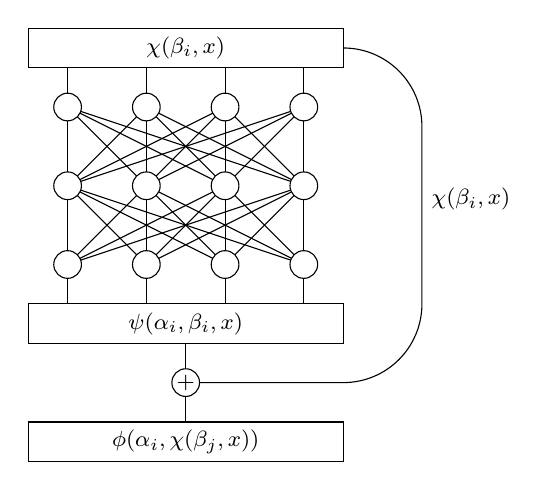
\begin{tikzpicture}
		\draw (0,2.75) node {\footnotesize $\chi(\beta_i,x)$};
		\draw (-2,2.5) -- (2,2.5) -- (2,3) -- (-2,3) -- (-2,2.5);
		\draw (-1.5,2.5) -- (-1.5,2);
		\draw (-0.5,2.5) -- (-0.5,2);
		\draw (0.5,2.5) -- (0.5,2);
		\draw (1.5,2.5) -- (1.5,2);
		%in
		\draw (-1.5,2) -- (-1.5,1);
		\draw (-1.5,2) -- (-0.5,1);
		\draw (-1.5,2) -- (0.5,1);
		\draw (-1.5,2) -- (1.5,1);
		\draw (-0.5,2) -- (-1.5,1);
		\draw (-0.5,2) -- (-0.5,1);
		\draw (-0.5,2) -- (0.5,1);
		\draw (-0.5,2) -- (1.5,1);
		\draw (0.5,2) -- (-1.5,1);
		\draw (0.5,2) -- (-0.5,1);
		\draw (0.5,2) -- (0.5,1);
		\draw (0.5,2) -- (1.5,1);
		\draw (1.5,2) -- (-1.5,1);
		\draw (1.5,2) -- (-0.5,1);
		\draw (1.5,2) -- (0.5,1);
		\draw (1.5,2) -- (1.5,1);
		%%% hidden
		\draw (-1.5,1) -- (-1.5,0);
		\draw (-1.5,1) -- (-0.5,0);
		\draw (-1.5,1) -- (0.5,0);
		\draw (-1.5,1) -- (1.5,0);
		\draw (-0.5,1) -- (-1.5,0);
		\draw (-0.5,1) -- (-0.5,0);
		\draw (-0.5,1) -- (0.5,0);
		\draw (-0.5,1) -- (1.5,0);
		\draw (0.5,1) -- (-1.5,0);
		\draw (0.5,1) -- (-0.5,0);
		\draw (0.5,1) -- (0.5,0);
		\draw (0.5,1) -- (1.5,0);
		\draw (1.5,1) -- (-1.5,0);
		\draw (1.5,1) -- (-0.5,0);
		\draw (1.5,1) -- (0.5,0);
		\draw (1.5,1) -- (1.5,0);
		%%%
		\draw (-1.5,-0.5) -- (-1.5,0);
		\draw (-0.5,-0.5) -- (-0.5,0);
		\draw (0.5,-0.5) -- (0.5,0);
		\draw (1.5,-0.5) -- (1.5,0);
		%%%
		\draw (-2,-0.5) -- (2,-0.5) -- (2,-1) -- (-2,-1) -- (-2,-0.5);
		\draw (-2,-2) -- (2,-2) -- (2,-2.5) -- (-2,-2.5) -- (-2,-2);
		\draw (0,-0.75) node {\footnotesize $\psi(\alpha_i,\beta_i,x)$};
		\draw (0,-1) -- (0,-2);
		\draw (2,2.75) to[out=0,in=90] (3,1.75) -- (3,-0.5) to[out=-90,in=0] (2,-1.5) -- (0,-1.5);
		\draw (0,-2.25) node {\footnotesize $\phi(\alpha_i,\chi(\beta_j,x))$};
		\draw (3,0.83) node[anchor=west] {\footnotesize $\chi(\beta_i,x)$};
		%layer in to 1
		\draw[fill=white] (-1.5,2) circle (5pt);
		\draw[fill=white] (-0.5,2) circle (5pt);
		\draw[fill=white] (0.5,2) circle (5pt);
		\draw[fill=white] (1.5,2) circle (5pt);
		\draw[fill=white] (-1.5,1) circle (5pt);
		\draw[fill=white] (-0.5,1) circle (5pt);
		\draw[fill=white] (0.5,1) circle (5pt);
		\draw[fill=white] (1.5,1) circle (5pt);
		\draw[fill=white] (-1.5,0) circle (5pt);
		\draw[fill=white] (-0.5,0) circle (5pt);
		\draw[fill=white] (0.5,0) circle (5pt);
		\draw[fill=white] (1.5,0) circle (5pt);
		\draw[fill=white] (0,-1.5) circle (5pt);
		\draw (0,-1.5) node {\footnotesize{$+$}};
	\end{tikzpicture}
	\caption{A residual block.}
	\label{fig:resblock}
\end{figure}
\subsection{Bottlenecked Residual Network}
The ResNet allows us to create much deeper networks, but the number of parameters stays the same as the linear model, making ResNets difficult to train (and especially the minimum of two linear layers. We can make a small modification to the ResNet that can resolve this, where there is an additional layer and the number of dimensions reduces in the middle (figure~\ref{fig:resbottle-block}). This forces the neural network to prioritize certain features and ignore ones that are not as necessary. Due to the shape this architecture makes, its referred to as a \textit{bottlenecked residual network} (ResBottle) (figure~\ref{fig:resbottle-block}).
\begin{figure}[ht]
	\centering
	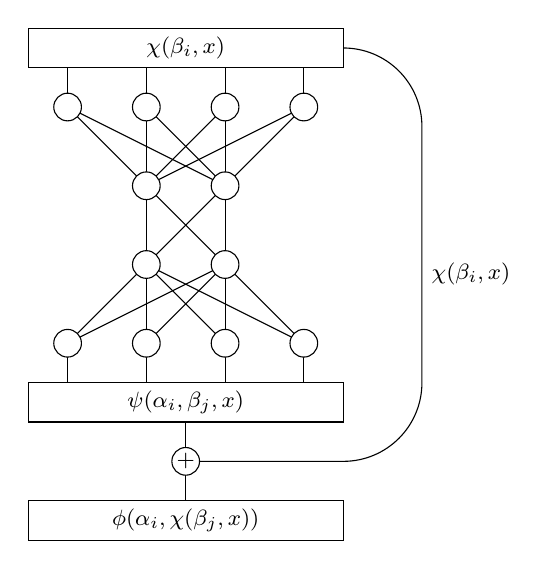
\begin{tikzpicture}
		\draw (1.5,1) -- (0.5,0);
		\draw (1.5,1) -- (-0.5,0);
		\draw (0.5,1) -- (0.5,0);
		\draw (0.5,1) -- (-0.5,0);
		\draw (-0.5,1) -- (0.5,0);
		\draw (-0.5,1) -- (-0.5,0);
		\draw (-1.5,1) -- (0.5,0);
		\draw (-1.5,1) -- (-0.5,0);
		\draw (-0.5,0) -- (-0.5,-1);
		\draw (-0.5,0) -- (0.5,-1);
		\draw (0.5,0) -- (-0.5,-1);
		\draw (0.5,0) -- (0.5,-1);
		\draw (1.5,-2) -- (0.5,-1);
		\draw (1.5,-2) -- (-0.5,-1);
		\draw (0.5,-2) -- (0.5,-1);
		\draw (0.5,-2) -- (-0.5,-1);
		\draw (-0.5,-2) -- (0.5,-1);
		\draw (-0.5,-2) -- (-0.5,-1);
		\draw (-1.5,-2) -- (0.5,-1);
		\draw (-1.5,-2) -- (-0.5,-1);
		%%%
		\draw (-1.5,1.5) -- (-1.5,1);
		\draw (-0.5,1.5) -- (-0.5,1);
		\draw (0.5,1.5) -- (0.5,1);
		\draw (1.5,1.5) -- (1.5,1);
		\draw (-1.5,-2.5) -- (-1.5,-2);
		\draw (-0.5,-2.5) -- (-0.5,-2);
		\draw (0.5,-2.5) -- (0.5,-2);
		\draw (1.5,-2.5) -- (1.5,-2);
		\draw (-2,-2.5) -- (2,-2.5) -- (2,-3) -- (-2,-3) -- (-2,-2.5);
		\draw (-2,1.5) -- (2,1.5) -- (2,2) -- (-2,2) -- (-2,1.5);
		%%%
		\draw (0,-4) -- (0,-3);
		\draw (-2,-4.5) -- (2,-4.5) -- (2,-4) -- (-2,-4) -- (-2,-4.5);
		%%%
		\draw[fill=white] (1.5,1) circle (5pt);
		\draw[fill=white] (0.5,1) circle (5pt);
		\draw[fill=white] (-0.5,1) circle (5pt);
		\draw[fill=white] (-1.5,1) circle (5pt);
		%%%
		\draw[fill=white] (0.5,0) circle (5pt);
		\draw[fill=white] (-0.5,0) circle (5pt);
		%%%
		\draw[fill=white] (0.5,-1) circle (5pt);
		\draw[fill=white] (-0.5,-1) circle (5pt);
		%%%
		\draw[fill=white] (1.5,-2) circle (5pt);
		\draw[fill=white] (0.5,-2) circle (5pt);
		\draw[fill=white] (-0.5,-2) circle (5pt);
		\draw[fill=white] (-1.5,-2) circle (5pt);
		%%%
		\draw (2,1.75) to[out=0,in=90] (3,0.75) -- (3,-2.5) to[out=-90,in=0] (2,-3.5) -- (0,-3.5);
		\draw[fill=white] (0,-3.5) circle (5pt);
		\draw (0,-3.5) node {\footnotesize $+$};
		\draw (0,1.75) node {\footnotesize $\chi(\beta_i,x)$};
		\draw (0,-2.75) node {\footnotesize $\psi(\alpha_i,\beta_j,x)$};
		\draw (0,-4.25) node {\footnotesize $\phi(\alpha_i, \chi(\beta_j,x))$};
		\draw (3,-1.12) node[anchor=west] {\footnotesize $\chi(\beta_i,x)$};
	\end{tikzpicture}
	\caption{A bottlenecked residual block.}
	\label{fig:resbottle-block}
\end{figure}
In the examples drawn (figures~\ref{fig:resblock} and~\ref{fig:resbottle-block}), there are 40 parameters in the ResNet, but only 28 parameters in the ResBottle. This allows us to either simplify the model, add more layers, or make the layers much wider without blowing up the number of parameters that need to be trained.
\subsection{Attention}
This will be the most complicated model to test. If we look at the structure of the data vector, there is a certain order to the data and correlation between the components. The data vectors are separated into redshift bins, and within each redshift bin are bins representing different scales. Thus, a NN that can learn sequences may be useful. Fortunately, there are NNs we encounter every day that use sequences: chatbots! The basis for this is usually attention networks~\cite{vaswani_attention_2017}. These work by examining dot products between vectors so that the output is directly related to the angle between the two vectors.

suppose we are given a sequence of input vectors, $x=(x_1,x_2,\ldots,x_n)$, then we can construct dot products of each $x_i$ and use them as coefficients for the output.
\begin{equation}
	y_k = (x_i \cdot x_j)x_k
\end{equation}
We can introduce generalize the dot product using linear transformations. That is, we can introduce the transformation matrices $W_Q$, $W_K$, $W_V$. Let $q_i = W_Q x_i$, $k_i = W_K x_i$, and $v_i = W_V x_i$. Then we can also write a dot product as 
\begin{equation}
	y_k = (q_i^T k_j)v_k
\end{equation}
Finally, we can introduce a non-linearity, which also keeps the outputs sequence $y$ normalized. By introducing the \textit{softmax} function.
\begin{equation}
	y_k = \mathrm{softmax}(q_i^T k_j / \sqrt{d})v_k
\end{equation}
where the softmax function is an exponential normalization given by
\begin{equation}
	\mathrm{softmax}(W)_i = \frac{e^{w_i}}{e^{\sum_i{w_i}}}
\end{equation}
and $d$ is the embedding dimension (i.e $W_K\in \mathbb{R}^{d_x\times d}$).
We allow the linear matrices $W_Q$, $W_K$, and $W_V$ to contain learnable components. We then pass each output $y_i$ to its own MLP. We also keep the skip connections describe in the residual network section. The attention together with the MLPs and skip connections is called a transformer block, drawn in figure~\ref{fig:attention}.
\begin{figure}[ht]
	\centering
	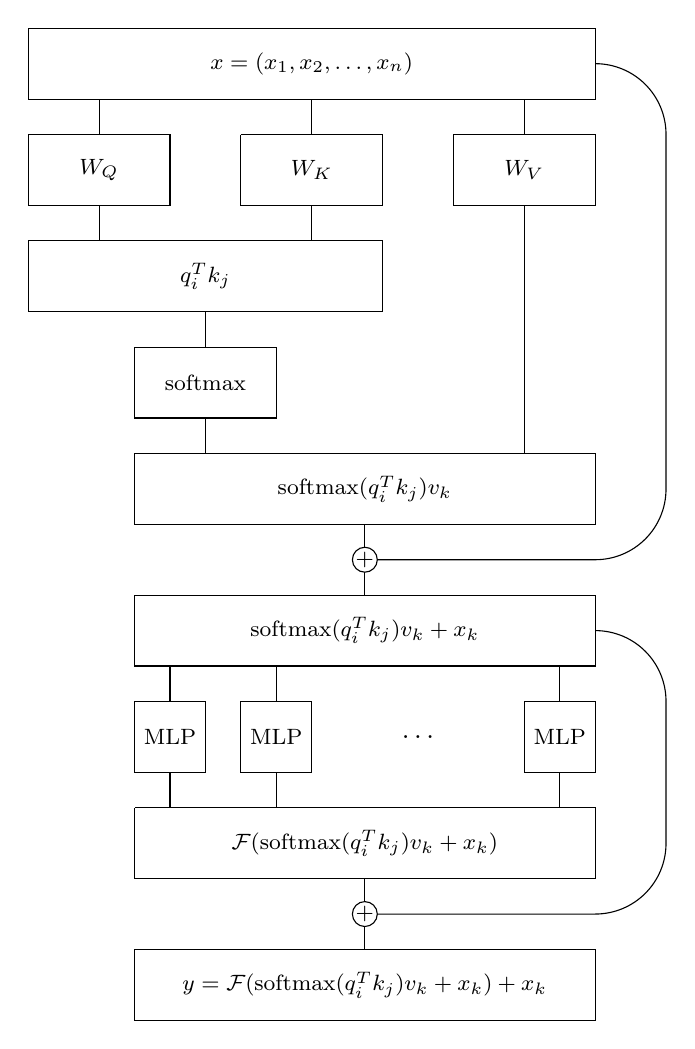
\begin{tikzpicture}[scale=0.9]
		%%curved skip lines
		\draw (8,2.5) to[out=0,in=90] (9,1.5) -- (9,-3.5) to[out=-90,in=0] (8,-4.5) -- (4.75,-4.5);
		\draw (8,-5.5) to[out=0,in=90] (9,-6.5) -- (9,-8.5) to[out=-90,in=0] (8,-9.5) -- (4.75,-9.5);
		%%input
		\draw (0,2) -- (8,2) -- (8,3) -- (0,3) -- (0,2);
		\draw (4,2.5) node {\footnotesize $x=(x_1,x_2,\dots,x_n)$};
		%%next!
		%\draw (1,4) node[anchor=south] {\footnotesize $x_i$};
		\draw (1,2) -- (1,1.5);
		\draw (1,1) node {\footnotesize $W_Q$};
		\draw (0,1.5) -- (0,0.5) -- (2,0.5) -- (2,1.5) -- (0,1.5);
		%\draw (4,4) node[anchor=south] {\footnotesize $x_j$};
		\draw (4,2) -- (4,1.5);
		\draw (4,1) node {\footnotesize $W_K$};
		\draw (3,1.5) -- (3,0.5) -- (5,0.5) -- (5,1.5) -- (3,1.5);
		%%next!
		\draw (1,0.5) -- (1,0);
		\draw (4,0.5) -- (4,0);
		\draw (5,-1) -- (0,-1) -- (0,0) -- (5,0) --  (5,-1);
		\draw (2.5,-0.5) node {\footnotesize $q_i^T k_j$};
		%%next!
		%\draw (7,4) node[anchor=south] {\footnotesize $x_k$};
		\draw (7,2) -- (7,1.5);
		\draw (7,1) node {\footnotesize $W_V$};
		\draw (6,1.5) -- (6,0.5) -- (8,0.5) -- (8,1.5) -- (6,1.5);
		%%next!
		\draw (2.5,-1) -- (2.5,-1.5);
		\draw (1.5,-1.5) -- (1.5,-2.5) -- (3.5,-2.5) -- (3.5,-1.5) -- (1.5,-1.5);
		\draw (2.5,-2) node {\footnotesize softmax};
		%%next!
		\draw (7,0.5) -- (7,-3);
		\draw (2.5,-2.5) -- (2.5,-3);
		\draw (1.5,-3) -- (1.5,-4) -- (8,-4) -- (8,-3) -- (1.5,-3);
		\draw (4.75,-3.5) node {\footnotesize $\mathrm{softmax}(q_i^T k_j)v_k$};
		%%skips!
		\draw (4.75,-4) -- (4.75,-5);
		\draw[fill=white] (4.75,-4.5) circle (5pt);
		\draw (4.75,-4.5) node {\footnotesize $+$};
		%mlps
		\draw (1.5,-5) -- (1.5,-6) -- (8,-6) -- (8,-5) -- (1.5,-5);
		\draw (4.75,-5.5) node {\footnotesize $\mathrm{softmax}(q_i^T k_j)v_k + x_k$};
		\draw (2,-6) -- (2,-6.5);
		\draw (1.5,-6.5) -- (1.5,-7.5) -- (2.5,-7.5) -- (2.5,-6.5) -- (1.5,-6.5);
		\draw (2,-7) node {\footnotesize MLP};
		\draw (3.5,-6) -- (3.5,-6.5);
		\draw (3,-6.5) -- (3,-7.5) -- (4,-7.5) -- (4,-6.5) -- (3,-6.5);
		\draw (3.5,-7) node {\footnotesize MLP};
		\draw (5.5,-7) node {$\hdots$};
		\draw (7.5,-6) -- (7.5,-6.5);
		\draw (7,-6.5) -- (7,-7.5) -- (8,-7.5) -- (8,-6.5) -- (7,-6.5);
		\draw (7.5,-7) node {\footnotesize MLP};
		%%last skip
		\draw (7.5,-7.5) -- (7.5,-8);
		\draw (3.5,-7.5) -- (3.5,-8);
		\draw (2,-7.5) -- (2,-8);
		\draw (1.5,-8) -- (1.5,-9) -- (8,-9) -- (8,-8) -- (1.5,-8);
		\draw (4.75,-8.5) node {\footnotesize $\mathcal{F}(\mathrm{softmax}(q_i^T k_j)v_k + x_k)$};
		\draw (4.75,-9) -- (4.75,-10);
		\draw (1.5,-10) -- (1.5,-11) -- (8,-11) -- (8,-10) -- (1.5,-10);
		\draw[fill=white] (4.75,-9.5) circle (5pt);
		\draw (4.75,-9.5) node {\footnotesize $+$};
		\draw (4.75,-10.5) node {\footnotesize $y = \mathcal{F}(\mathrm{softmax}(q_i^T k_j)v_k + x_k)+x_k$};
	\end{tikzpicture}
	\caption{A transformer block}
	\label{fig:attention}
\end{figure}

\section{Results}
We present the results in two sections: the first will be about the training and testing results, and the second comparing between a cocoa chain and an emulated chain. For training and testing, we use the "train, validate, test" approach. We generate three completely independent chains, one is only for training the model, and is a high temperature chain with data well beyond the expected range. The second is used to validate that the model is not overfitting as the training proceeds. The last set is another high temperature chain (but not as high as the training) which is used to test the model as if it were being used as normal. The testing involves reintroducing specific analysis choices, such as the scale cut.

When deciding on which model to use, we want to look at several aspects:
\begin{itemize}
	\item The number of parameters. The more parameters we have, the longer it takes to train, and the longer it takes to evaluate. This will make it difficult for groups without top-of-the-line equipment.
	\item The $\Delta\chi^2$ between the emulator and accepted computational methods. Many experiments have a $\chi^2$ requirement for their emulators; for example, DES requires $\Delta\chi^2<0.3$ between any approximations and CosmoLike.
	\item Generalizability. As we increase the volume covered in the parameter space, which models are able to keep up with the growing modelling volume? Which models can handle more input parameters (which many models need, such as early dark energy with $\sim10$ extra parameters).
\end{itemize}
These get analyzed on the test data set. Because of the second point above, we define the loss function as the difference in $\chi^2$ between the emulator and CosmoLike. This allows us to capture the covariance of the data.
\subsection{Training and Testing}
We train the emulator by using a rough Gaussian approximation on the cosmological parameters. The benefit is that running MCMC chains on a simple Gaussian without the need for CosmoLike is extremely fast. Given the samples, the data vector calculation is trivially parallelizable, so the entire process is significantly faster than running an MCMC in CosmoLike. 

% First, we examine the training and validation loss at each epoch. The training loss is the average loss of all batches in an epoch. Figure~\ref{fig:train_loss_resnet} displays the training loss of a ResNet model with 3 ResNet blocks and 256 neurons in each hidden layer. In this case, we can see a consistent decline in both the training and validation loss. Additionally, we can see the points where the learning rate decreases (see epoch 50 and epoch 85 in figure~\ref{fig:train_loss_resnet}) which occur when validation loss plateaus, following the expected behavior. This demonstrates that we are likely not overfitting the training data.
% \begin{figure}[tb]
% 	\centering
% 	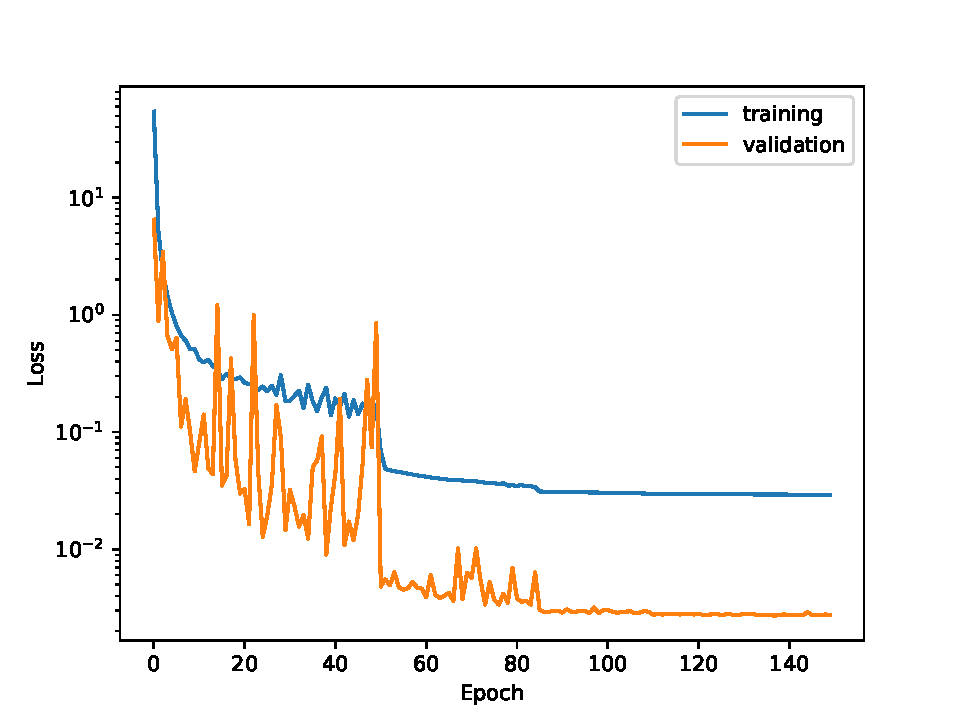
\includegraphics[width=0.9\textwidth]{plots/losses_resnet_3_256.pdf}
% 	\caption{Loss of a ResNet model with 3 ResNet blocks and 256 neurons in each layer.}
% 	\label{fig:train_loss_resnet}
% \end{figure}
% Using a trained model, we evaluate $\Delta\chi^2$ on the test data, a $T=8$ Gaussian approximated chain (figure~\ref{fig:testing_loss}). As we can see, our model is able to generalize well to a $T=8$ chain. 
% \begin{figure}[tb]
% 	\centering
% 	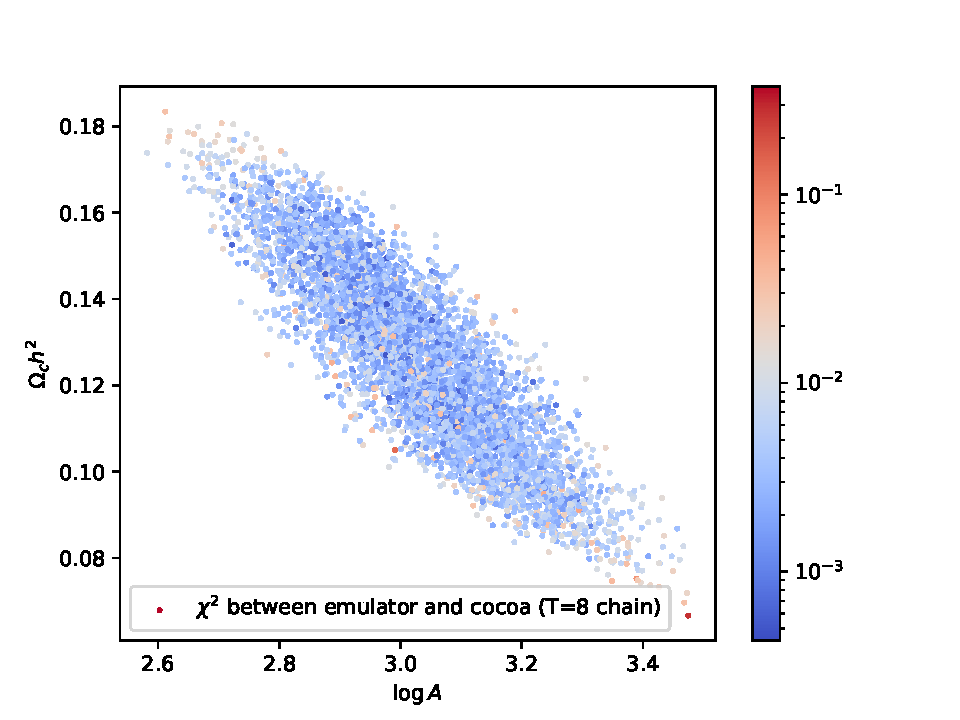
\includegraphics[width=0.9\textwidth]{plots/cosmic_shear_resnet_nlayer_3_intdim_256.pdf}
% 	\caption{Testing loss on a $T=8$ chain.}
% 	\label{fig:testing_loss}
% \end{figure}
First, we tested the different architectures by training them on a $T=16$ chain. The testing was done on a $T=8$ chain. we find that the ResNet is able to consistently perform the best of the three basic architectures. The number of layers and width of the layers makes minimal difference. An interesting result comes from the wide MLP architectures, where the testing loss suddenly spikes. This is likely due to either vanishing gradients or some poorly chosen hyperparameters of the model. Regardless of the issue, this instability is not desirable, as we would like to provide a framework for others to build emulators of their own, and fine-tuning hyperparameters adds significant difficulty to this process. The ResBottle consistently performs worse than the others, meaning the information the model learns in necessary to correctly model the final data vector. This is perhaps unsurprising for our relatively small models, but if one needs to create much wider networks, the ResBottle may be the only way to keep the number of parameters reasonable. Nevertheless, the ResBottle has a satisfactory performance overall.
% \begin{figure}[htb]
% 	\centering
% 	\begin{subfigure}[b]{0.4\textwidth}
% 		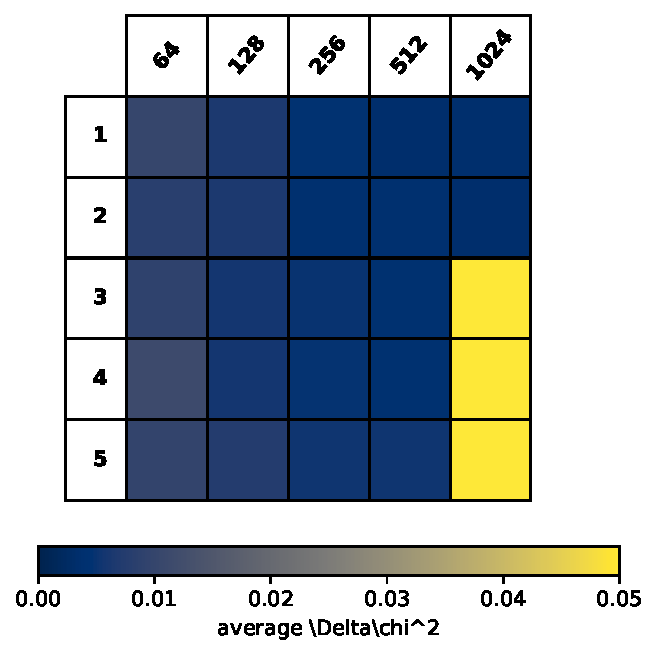
\includegraphics[width=\textwidth]{plots/model_table_mlp.pdf}
% 		\caption{MLP average loss}
% 		\label{fig:mlp_table}
% 	\end{subfigure}
% 	\begin{subfigure}[b]{0.4\textwidth}
% 		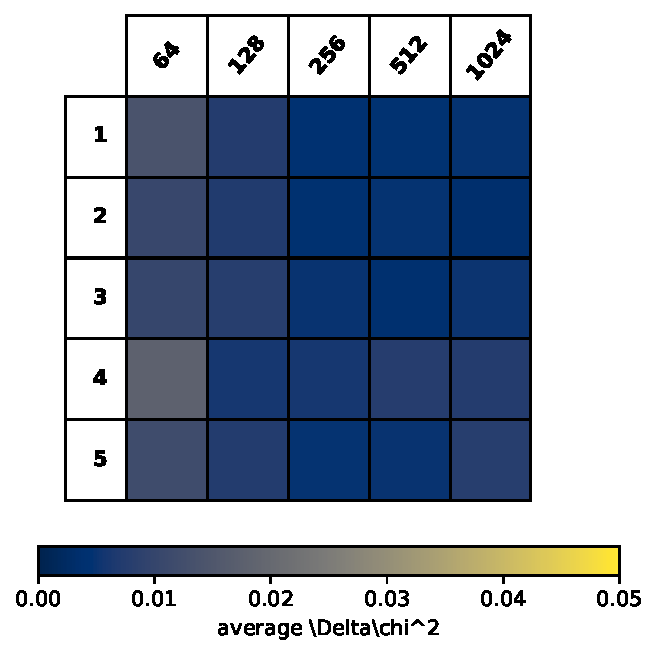
\includegraphics[width=\textwidth]{plots/model_table_resnet.pdf}
% 		\caption{ResNet average loss}
% 		\label{fig:resnet_table}
% 	\end{subfigure}
% 	\begin{subfigure}[b]{0.8\textwidth}
% 		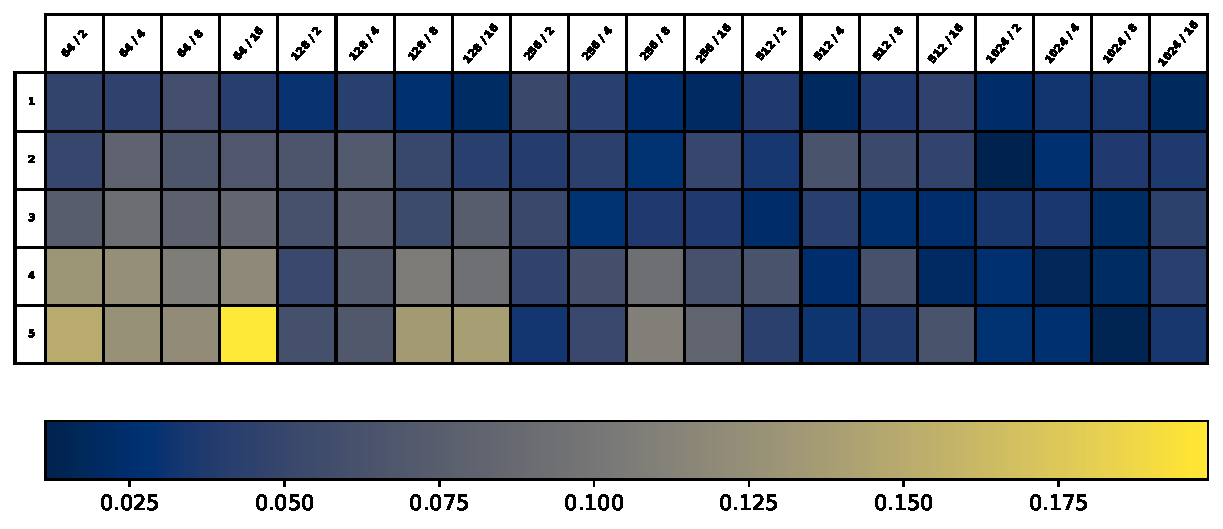
\includegraphics[width=\textwidth]{plots/model_table_resbottle.pdf}
% 		\caption{ResBottle average loss}
% 		\label{fig:resbottle_table}
% 	\end{subfigure}
% 	\label{fig:model_tables}
% \end{figure}
\begin{figure}[htb]
	\centering
	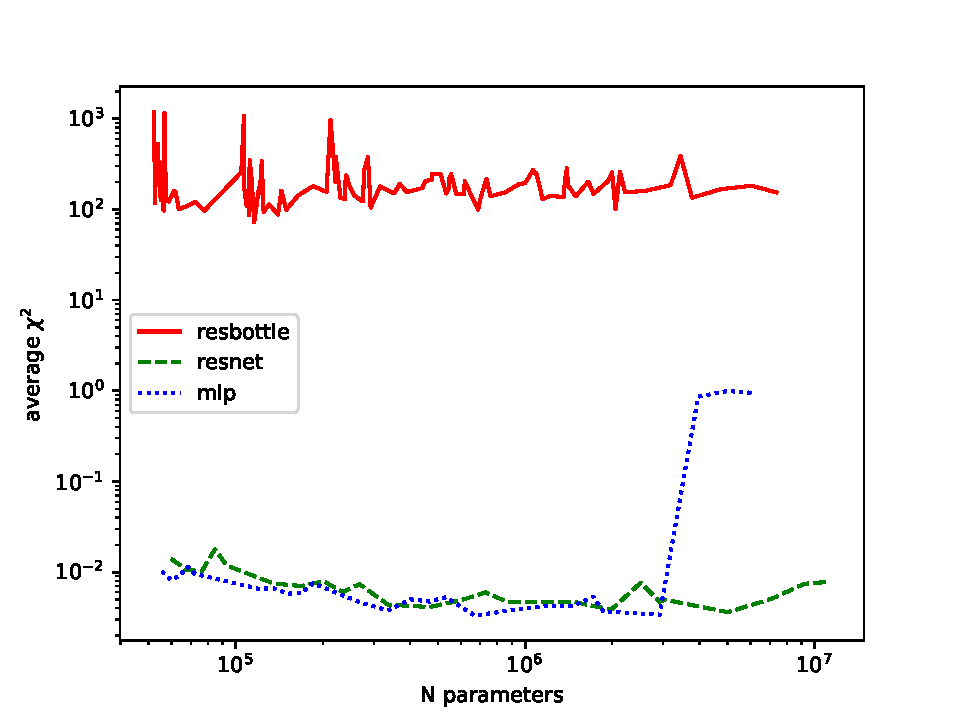
\includegraphics[width=0.8\textwidth]{plots/avg_chi2_v_n_params_new.pdf}
	\caption{Average $\Delta\chi^2$ as a function of the number of parameters for each architecture.}
	\label{fig:avg_chi2_nparams}
\end{figure}

Additionally, we can test how high of a temperature we can train on and still get satisfactory performance. We noticed the MLP, ResNet, and ResBottle models fail to train on a $T=128$ chain (figure~\ref{fig:avg_chi2_nparams_t128}).
\begin{figure}[!tb]
	\centering
	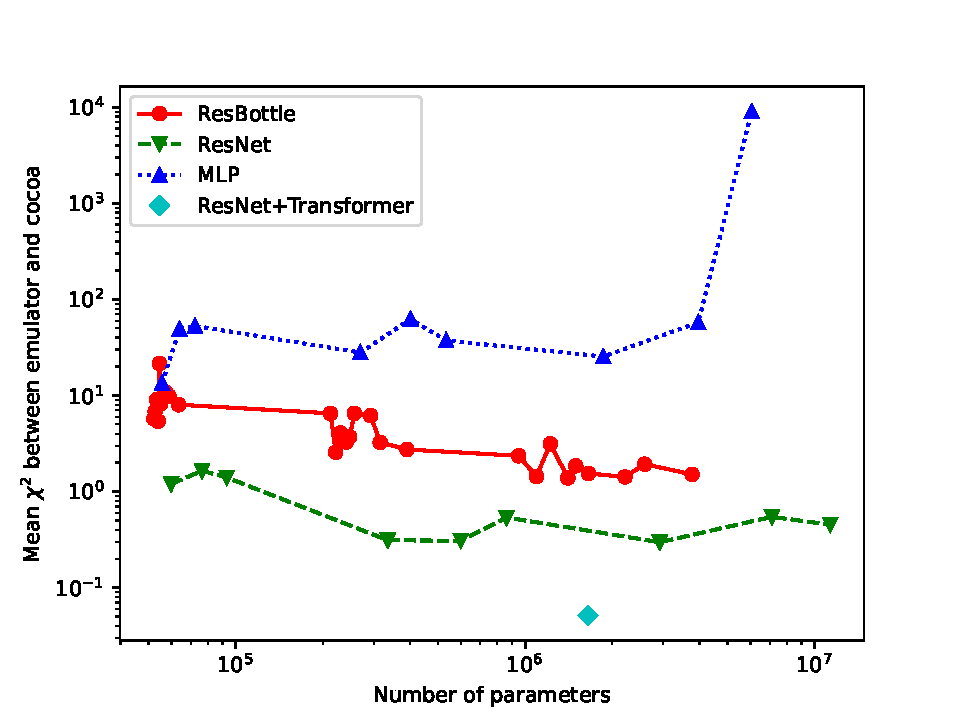
\includegraphics[width=0.8\textwidth]{plots/avg_chi2_v_n_params_T64.pdf}
	\caption{Average $\Delta\chi^2$ of a $T=64$ chain using emulators trained on a $T=128$ chain.}
	\label{fig:avg_chi2_nparams_t128}
\end{figure} 
We added the transformer block to the $T=128$ training to see the gain in performance attributed to the complex model. We find adding a transformer block to the end of the 3 ResBlock model (figure~\ref{fig:full_arch}) is able to give satisfactory performance when training on $T=128$ and testing on $T=64$ chains.
\begin{figure}[!tb]
	\centering
	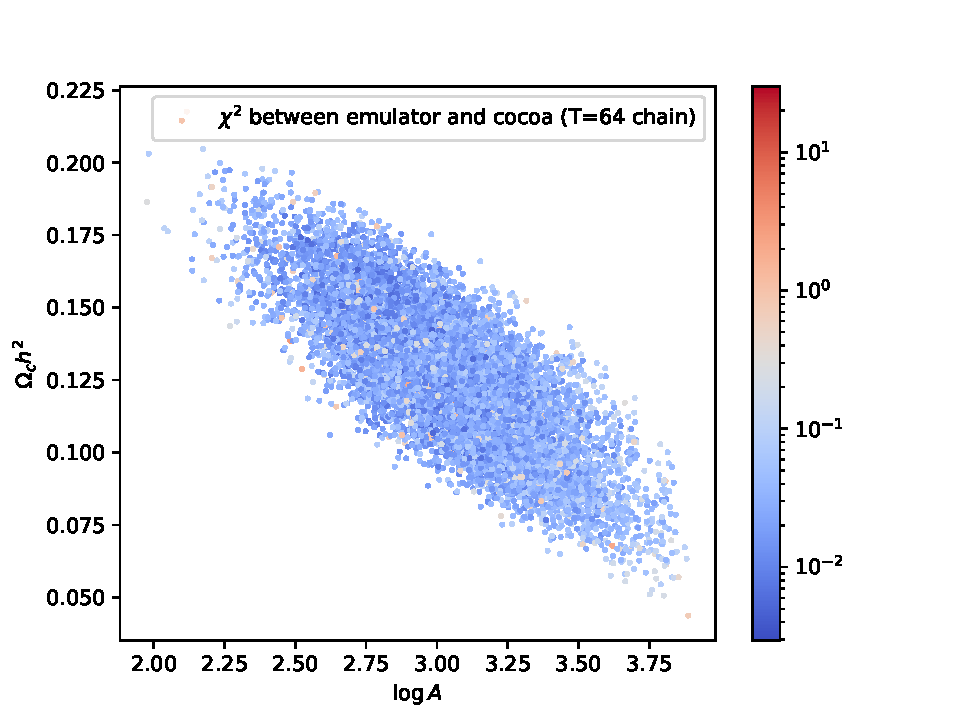
\includegraphics[width=0.8\textwidth]{plots/T64_attention_stuff.pdf}
	\caption{Marginalized distribution of $\Delta\chi^2$ of a $T=64$ chain using the model in figure~\ref{fig:full_arch} trained on a $T=128$ chain.}
	\label{fig:testing_attention_t128}
\end{figure}

\begin{figure}[!tb]
	\centering
	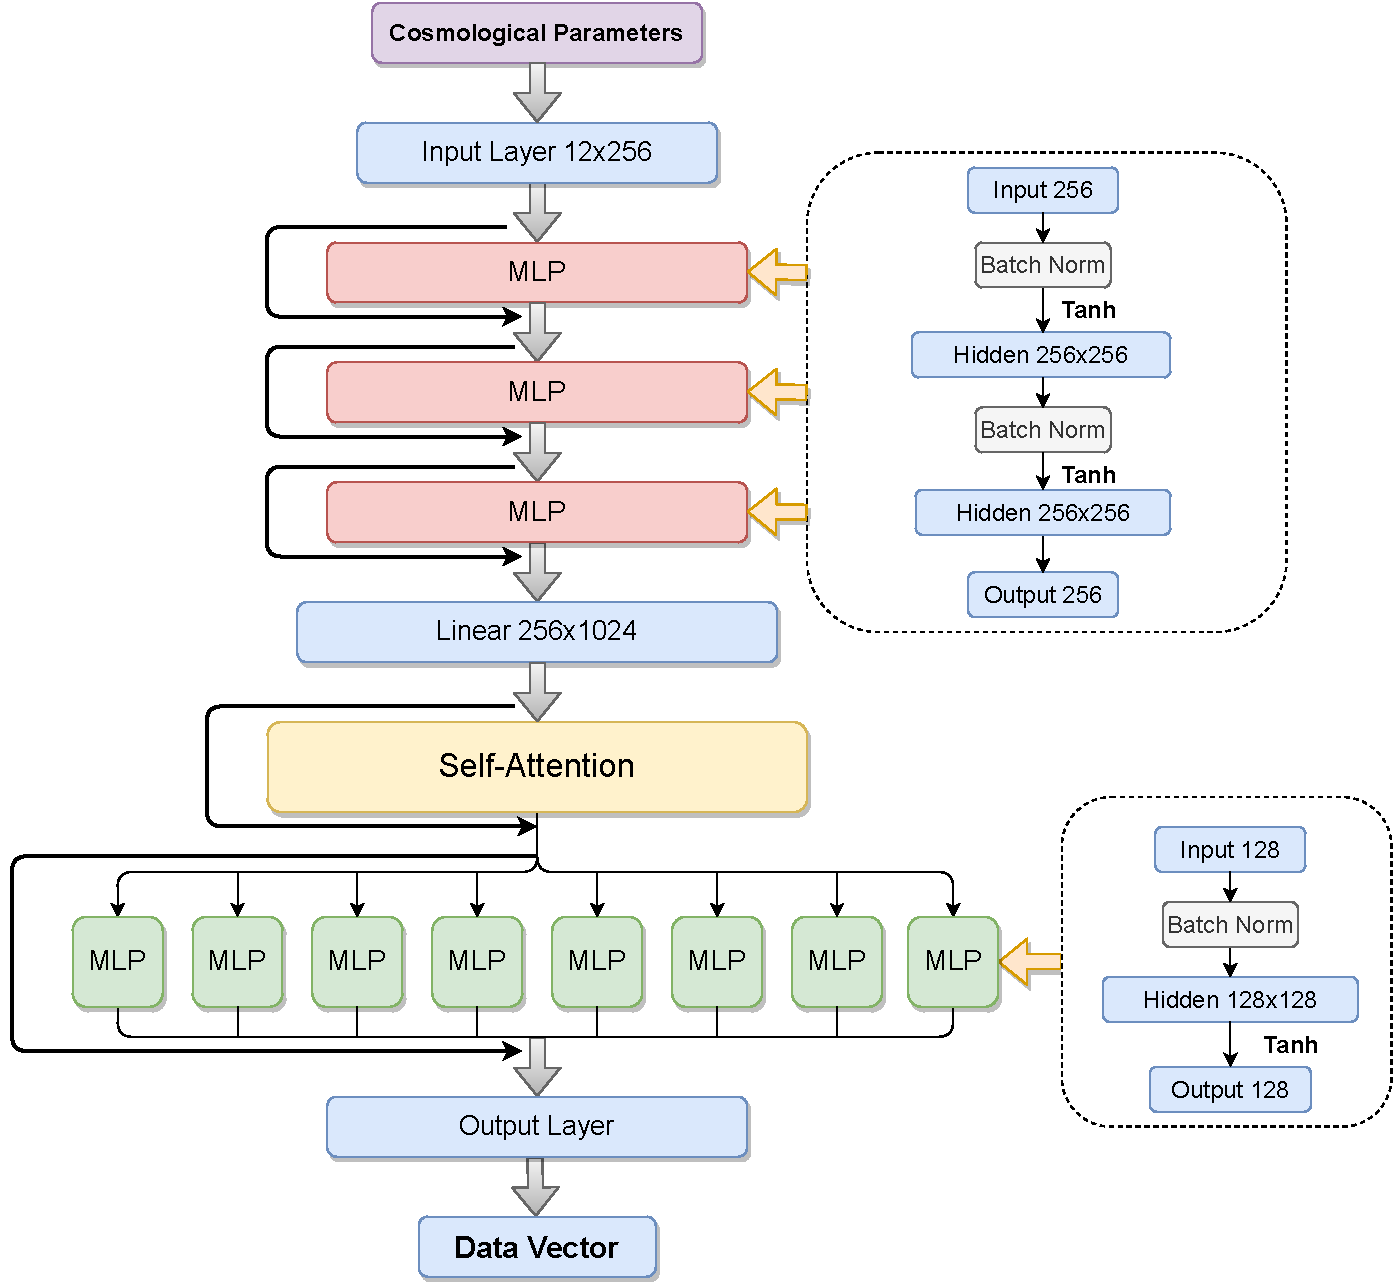
\includegraphics[width=0.8\textwidth]{plots/Untitled Diagram.drawio-5.pdf}
	\caption{Full NN architecture used for training on high temperature chains. Comprised of three ResBlocks of size 256, and a transformer block with 8 heads, each with a size of 128.}
	\label{fig:full_arch}
\end{figure}

This demonstrates the importance of making an intelligent choice for emulator architecture. By implementing the self attention, we were able to greatly increase the amount of the $\Lambda$CDM parameter space covered by the emulator. The additional volume will allow one to use emulators, even on real data, where the data vectors can be shifted greatly from things such as baryon contamination. We would like to continue this to see how this architecture will hold for more complex extensions to $\Lambda$CDM, such as early dark energy, which adds $\sim10$ parameters. We are also working with a team on using this architecture to model much larger data vectors.

\section{Application to Tension Calibration}
In this section, I will apply the use of emulators to do a first study of tension metric error. By shifting the parameters and generating noise realizations on the data, we can get a sense of how the error in the data propagates to error in the tension. This will provide additional information as to which tension metrics perform best, as well as adding context to how tension may vary given new measurements. Additionally, given that $n_\sigma=0$ means no tension, the error are tension metrics will allow us to gauge how reasonable it may be for the tension to be resolved by additional identical measurements.

I will be shifting the LSST fiducial cosmology to $\pm5\sigma$ in both the $\sigma_8$ and $\Omega_m$ directions. At each of these shifts, I will compute 256 noise realizations on LSST cosmic shear and Planck TTTEEE using the respective data covariances. Finally, the tension will be computed using the methods described in section~\ref{sec:tension_metrics}. Due to time constraints, the chains for the shifts will not be presented in this thesis. I will, however, demonstrate this method using the fiducial cosmologies of LSST and Planck.

The autocorrelation $\tau$ for the MCMC sampler was measured to be $\tau\sim1000$, thus we need to run the chain for about 50000 steps ($50\tau$) using the enseble sampler in $\textsc{Emcee}$. Each chain has 120 walkers, resulting in a total runtime of just 8 hours on a single 40 core CPU. The joint chains used for $Q_{\mathrm{UDM}}$ were run for just 5000 steps, since that is sufficient for the mean and covariance to converge. 
\begin{figure}[tb]
	\centering
	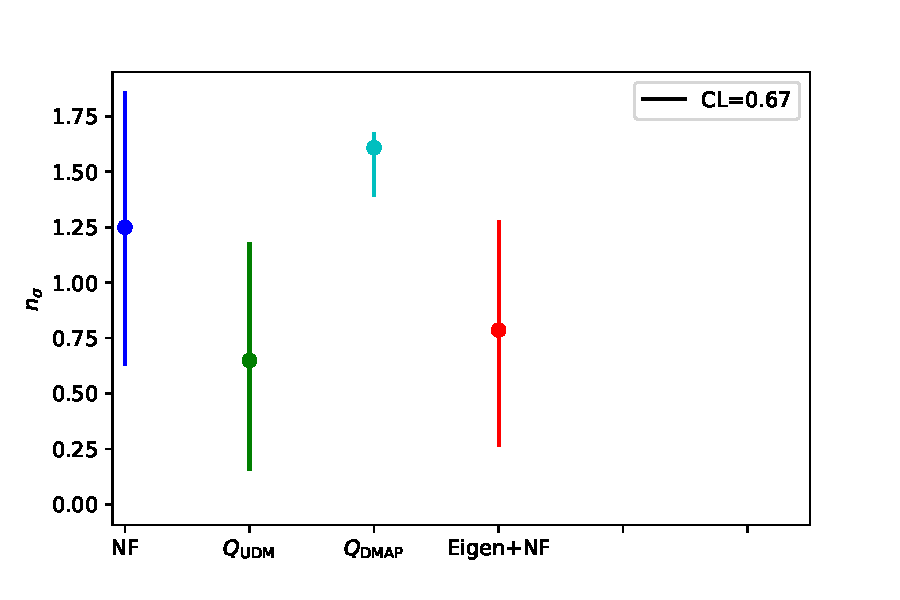
\includegraphics[width=0.8\textwidth]{plots/metrics_new.pdf}
	\caption{tension metrics error}
	\label{fig:tension_metrics_error}
\end{figure}

We see that, up to noise realizations, the different tension metrics are nearly indistinguishable. Both Planck and LSST are nearly gaussian, but for more non-gaussian posteriors (such as DES), the difference between the parameter difference and other metrics may be more significant. We also see that the tension can be reduced by the experimental noise, but cannot be reduced to 0. It remains to compute the tension for noise realizations on the cosmologies with shifted $\Omega_m$ and $\sigma_8$.

The result for $Q_{\mathrm{UDM}}$ is significantly lower than the other metrics. This is likely becuase it makes the assumption that the posteriors are Gaussian, where as the tension can hide in the non-Gaussian parts of the posterior. Additionally, the error bar on $Q_{\mathrm{DMAP}}$ is much smaller. This requires some investigation into the distribution of the maximum-a-posteriori of the noise realizations. While noise realizations on the data generate large shifts in the posterior, the same is not necessarily true for the maximum-a-posteriori.

\section{Conclusion}
We are able to implement a NN emulator that works on temperatures as high as 128 by using the chatGPT inspired transformer block. Using the emulators, we can ensure that the posteriors are robust for noise realizations on the data. Using these noise realizations we can compute the error on the tension metrics.

A future study will be done creating emulators for different extension models which push the number of input parameters, as well as different data sets which push the number of output parameters. Using this baseline framework, we can also rapidly analyze smaller extensions, such as the geometry and growth split detailed in chapter 4.










%%%%%%%%%%%%%%%%%%%%%%%%%%%%%%%%%%%%%%%%%%%%%%%%%%%%%%%%%%%%%%%%%%%%%%%%%%%%%%%%
\bibliographystyle{unsrtnat}{}
\renewcommand{\baselinestretch}{1}
\normalsize

\clearpage
\newpage
\phantomsection%
\addcontentsline{toc}{chapter}{\numberline{}{Bibliography}}%
\bibliography{bib.bib}

\clearpage
\newpage

\appendix
\include{sections/appendixSdkr}
%\include{sections/appendixNOON}

\end{document}


